
\documentclass[acmsmall,review]{acmart}\settopmatter{printfolios=true,printccs=false,printacmref=false}

\usepackage{proof}
\usepackage{amssymb}
\usepackage{amsmath}
\usepackage[utf8]{inputenc}
\usepackage{pdflscape}
\usepackage{multirow,bigdelim}
\newcommand{\blank}{\mathord{\hspace{1pt}\text{--}\hspace{1pt}}} %from the book
\newcommand{\Set}{\mathsf{Set}}
\newcommand{\Id}{\mathsf{Id}}
\newcommand{\ra}{\rightarrow}
\newcommand{\A}{\mathsf{A}}
\newcommand{\F}{\mathsf{F}}
\renewcommand{\S}{\mathsf{S}}
\renewcommand{\O}{\mathsf{O}}
\newcommand{\M}{\mathsf{M}}
\newcommand{\id}{\mathsf{id}}
\newcommand{\ass}{\mathsf{ass}}
\newcommand{\idl}{\mathsf{idl}}
\newcommand{\idr}{\mathsf{idr}}
\newcommand{\con}{\mathsf{con}}
\newcommand{\elim}{\mathsf{elim}}
\newcommand{\Con}{\mathsf{Con}}
\newcommand{\Ty}{\mathsf{Ty}}
\newcommand{\Tms}{\mathsf{Sub}}
\newcommand{\Sub}{\mathsf{Sub}}
\newcommand{\Tm}{\mathsf{Tm}}
\newcommand{\nat}{\mathsf{nat}}
\newcommand{\lb}{\langle}
\newcommand{\rb}{\rangle}
\renewcommand{\U}{\mathsf{U}}
\newcommand{\El}{\mathsf{El}}
\newcommand{\wk}{\mathsf{wk}}
\newcommand{\vz}{\mathsf{vz}}
\newcommand{\vs}{\mathsf{vs}}
\newcommand{\Ra}{\Rightarrow}
\renewcommand{\tt}{\mathsf{tt}}
\newcommand{\proj}{\mathsf{proj}}
\newcommand{\refl}{\mathsf{refl}}
\newcommand{\J}{\mathsf{J}}
\newcommand{\tr}{\mathsf{tr}}
\newcommand{\trans}{\mathbin{\raisebox{0.2ex}{$\displaystyle\centerdot$}}}
\newcommand{\ap}{\mathsf{ap}}
\newcommand{\apd}{\mathsf{apd}}
\newcommand{\APP}{\mathsf{app}}
\newcommand{\app}{\mathop{{\scriptstyle @}}}
\newcommand{\rec}{\mathsf{rec}}
\renewcommand{\C}{\mathsf{C}}
\newcommand{\R}{\mathsf{R}}
\newcommand{\E}{\mathsf{E}}
\newcommand{\transp}{\mathsf{transp}}
\newcommand{\Pim}{\hat{\Pi}}
\newcommand{\Ram}{\mathbin{\hat{\Ra}}}
\newcommand{\appm}{\mathop{\hat{\app}}}
\newcommand{\Pii}{{\Pi}^*}
\newcommand{\lami}{{\lambda}^*}
\newcommand{\appi}{\mathop{{\app}^*}}
\newcommand{\reflect}{\mathsf{reflect}}
\newcommand{\funext}{\mathsf{funext}}
\newcommand{\UIP}{\mathsf{UIP}}
\newcommand{\coe}{\mathsf{coe}}
\newcommand{\LET}{\mathsf{let}}
\newcommand{\IN}{\mathsf{in}}
\newcommand{\N}{\mathbb{N}}
\newcommand{\D}{\mathsf{D}}
\newcommand{\K}{\mathsf{K}}
\newcommand{\Eq}{\mathsf{Eq}}
\newcommand{\mk}{\mathsf{mk}}
\newcommand{\unk}{\mathsf{unk}}
\newcommand{\0}{\mathit{0}}
\newcommand{\1}{\mathit{1}}
\newcommand{\eqreflect}{\mathsf{eqreflect}}

\usepackage{tikz}
\usetikzlibrary{arrows,
                calc,
                decorations.pathreplacing,
                calligraphy,% had to be after decorations.pathreplacing
                matrix,
                positioning
                }

\allowdisplaybreaks

%% setting \sqcdot as HoTT-book-style transitivity
\makeatletter
\DeclareRobustCommand{\sqcdot}{\mathbin{\mathpalette\morphic@sqcdot\relax}}
\newcommand{\morphic@sqcdot}[2]{%
  \sbox\z@{$\m@th#1\centerdot$}%
  \ht\z@=.33333\ht\z@
  \vcenter{\box\z@}%
}
\makeatother


%% Journal information
%% Supplied to authors by publisher for camera-ready submission;
%% use defaults for review submission.
\acmJournal{PACMPL}
\acmVolume{1}
\acmNumber{CONF} % CONF = POPL or ICFP or OOPSLA
\acmArticle{1}
\acmYear{2018}
\acmMonth{1}
\acmDOI{} % \acmDOI{10.1145/nnnnnnn.nnnnnnn}
\startPage{1}

%% Copyright information
%% Supplied to authors (based on authors' rights management selection;
%% see authors.acm.org) by publisher for camera-ready submission;
%% use 'none' for review submission.
\setcopyright{none}

\bibliographystyle{ACM-Reference-Format}
%% Citation style
%% Note: author/year citations are required for papers published as an
%% issue of PACMPL.
\citestyle{acmauthoryear}   %% For author/year citations


%%%%%%%%%%%%%%%%%%%%%%%%%%%%%%%%%%%%%%%%%%%%%%%%%%%%%%%%%%%%%%%%%%%%%%
%% Note: Authors migrating a paper from PACMPL format to traditional
%% SIGPLAN proceedings format must update the '\documentclass' and
%% topmatter commands above; see 'acmart-sigplanproc-template.tex'.
%%%%%%%%%%%%%%%%%%%%%%%%%%%%%%%%%%%%%%%%%%%%%%%%%%%%%%%%%%%%%%%%%%%%%%

%% Some recommended packages.
\usepackage{booktabs}   %% For formal tables:
                        %% http://ctan.org/pkg/booktabs
\usepackage{subcaption} %% For complex figures with subfigures/subcaptions
                        %% http://ctan.org/pkg/subcaption


\begin{document}

%% Title information
\title{Constructing Quotient Inductive-Inductive Types}

%% Author information
%% Contents and number of authors suppressed with 'anonymous'.
%% Each author should be introduced by \author, followed by
%% \authornote (optional), \orcid (optional), \affiliation, and
%% \email.
%% An author may have multiple affiliations and/or emails; repeat the
%% appropriate command.
%% Many elements are not rendered, but should be provided for metadata
%% extraction tools.

%% Author with single affiliation.
\author{Thorsten Altenkirch}
%\authornote{with author1 note}          %% \authornote is optional;
                                        %% can be repeated if necessary
%\orcid{nnnn-nnnn-nnnn-nnnn}             %% \orcid is optional
\affiliation{
%  \position{Position1}
  \department{School of Computer Science}              %% \department is recommended
  \institution{University of Nottingham}            %% \institution is required
%  \streetaddress{Street1 Address1}
%  \city{City1}
%  \state{State1}
%  \postcode{Post-Code1}
  \country{United Kingdom}                    %% \country is recommended
}
\email{Thorsten.Altenkirch@nottingham.ac.uk}          %% \email is recommended

%% Author with two affiliations and emails.
\author{Ambrus Kaposi}
%\authornote{with author2 note}          %% \authornote is optional;
                                        %% can be repeated if necessary
\orcid{0000-0001-9897-8936}             %% \orcid is optional
\affiliation{
  %\position{Position2a}
  \department{Department of Programming Languages and Compilers}             %% \department is recommended
  \institution{E{\"o}tv{\"o}s Lor{\'a}nd University}           %% \institution is required
%  \streetaddress{Street2a Address2a}
  \city{Budapest}
%  \state{State2a}
%  \postcode{Post-Code2a}
  \country{Hungary}                   %% \country is recommended
}
\email{akaposi@inf.elte.hu}         %% \email is recommended

\author{Andr{\'a}s Kov{\'a}cs}
%\authornote{with author2 note}          %% \authornote is optional;
                                        %% can be repeated if necessary
\orcid{0000-0002-6375-9781}             %% \orcid is optional
\affiliation{
  %\position{Position2a}
  \department{Department of Programming Languages and Compilers}             %% \department is recommended
  \institution{E{\"o}tv{\"o}s Lor{\'a}nd University}           %% \institution is required
%  \streetaddress{Street2a Address2a}
  \city{Budapest}
%  \state{State2a}
%  \postcode{Post-Code2a}
  \country{Hungary}                   %% \country is recommended
}
\email{kovacsandras@inf.elte.hu}         %% \email is recommended


%% Abstract
%% Note: \begin{abstract}...\end{abstract} environment must come
%% before \maketitle command
\begin{abstract}
Quotient inductive-inductive types (QIITs) generalise inductive types
in two ways: a QIIT can have more than one sort and the later sorts
can be indexed over the previous ones. In addition, equality
constructors are also allowed. We work in a setting with uniqueness of
identity proofs, hence we use the term QIIT instead of higher
inductive-inductive type. An example of a QIIT is the well-typed
(intrinsic) syntax of type theory quotiented by conversion. In this
paper first we specify finitary QIITs using a domain-specific type
theory which we call the theory of signatures. The syntax of the
theory of signatures is given by a QIIT as well. Then, using this
syntax we show that all specified QIITs exist and they have a
dependent elimination principle. We also show that algebras of a
signature form a category with families (CwF) and use the internal
language of this CwF to show that dependent elimination is equivalent
to initiality.
\end{abstract}


%% 2012 ACM Computing Classification System (CSS) concepts
%% Generate at 'http://dl.acm.org/ccs/ccs.cfm'.
\begin{CCSXML}
<ccs2012>
<concept>
<concept_id>10011007.10011006.10011008</concept_id>
<concept_desc>Software and its engineering~General programming languages</concept_desc>
<concept_significance>500</concept_significance>
</concept>
<concept>
<concept_id>10003456.10003457.10003521.10003525</concept_id>
<concept_desc>Social and professional topics~History of programming languages</concept_desc>
<concept_significance>300</concept_significance>
</concept>
</ccs2012>
\end{CCSXML}

\ccsdesc[500]{Software and its engineering~General programming languages}
\ccsdesc[300]{Social and professional topics~History of programming languages}
%% End of generated code


%% Keywords
%% comma separated list
\keywords{homotopy type theory, inductive-inductive types, higher inductive types, quotient inductive types, logical relations, category with families, generalised algebraic theory}  %% \keywords are mandatory in final camera-ready submission

%% \maketitle
%% Note: \maketitle command must come after title commands, author
%% commands, abstract environment, Computing Classification System
%% environment and commands, and keywords command.
\maketitle


\section{Introduction}

\label{sec:intro}

A quotient inductive-inductive type (QIIT) can be seen as a
multi-sorted algebraic theory where sorts can be indexed over each
other. An example of a QIIT is the following well-typed (intrinsic)
syntax of a small type theory.
\begin{alignat*}{5}
  & \Con && : \Set \\
  & \Ty && : \Con\ra\Set \\
  & \cdot && : \Con \\
  & \rhd && : (\mathit{\Gamma}:\Con)\ra\Ty\,\mathit{\Gamma}\ra\Con \\
  & \U && : (\mathit{\Gamma}:\Con)\ra\Ty\,\mathit{\Gamma} \\
  & \Sigma && : (\mathit{\Gamma}:\Con)\ra(A:\Ty\,\mathit{\Gamma})\ra\Ty\,(\mathit{\Gamma}\rhd A)\ra\Ty\,\mathit{\Gamma} \\
  & \mathsf{eq} && : (\mathit{\Gamma}:\Con)\ra(A:\Ty\,\mathit{\Gamma})\ra(B:\Ty\,(\mathit{\Gamma}\rhd A))\ra (\Gamma\rhd A \rhd B = \Gamma\rhd \Sigma\,\Gamma\,A\,B)
\end{alignat*}
It has two sorts: contexts ($\Con$) and types ($\Ty$). The latter is
indexed over the former: to talk about a type we need to say which
context it lives in. There is an empty context $\cdot$ and context
extension $\rhd$ which takes a context and a type in that context and
returns the extended context. Note that we cannot turn this QIIT into
two inductive types defined one after the other because the
$\Con$-constructor $\rhd$ refers to $\Ty$, hence $\Con$ and $\Ty$ must
be defined \emph{at the same time}. There is a constructor for a base
type $\U$ in any context and a constructor for $\Sigma$ types. This
takes a context (this could be made an implicit parameter), a type $A$
in that context and a type in the context extended by $A$ and returns
a type in the original context. The third argument of $\Sigma$ shows a
pattern which does not appear in inductive types or indexed inductive
types: a constructor refers to a previous constructor (in our case
$\rhd$). Finally, there is an equality constructor which states the
unusual equality (included here for illustration) that extending a
context twice is the same as extending by a $\Sigma$ type. Equality
constructors can only target one of the sorts. The constructor
$\mathsf{eq}$ quotients contexts so that for any $\Gamma$, $A$ and $B$
it becomes impossible to distinguish $(\Gamma\rhd A \rhd B)$ and
$(\Gamma\rhd \Sigma\,\Gamma\,A\,B)$ -- this is ensured by the
eliminator of the QIIT as shown below. The equality constructor also
refers to previous constructors. This small example can be extended to
the full syntax of type theory as shown in \cite{ttintt}.

In this paper we define the {\em theory of signatures}, a small type
theory. It is itself given as a QIIT, and we show that if a type
theory supports this QIIT, then it supports all finitary QIITs. This
is analogous to the following results: if a type theory has W-types
\cite{abbot05containers}, then it has all inductive types; if a type
theory has indexed W-types \cite{morris09indexed}, then it has all
indexed inductive types.

The theory of signatures is a restriction of the theory of codes in
\cite{kaposi_et_al:LIPIcs:2018:9190}. A signature for a QIIT is given
by a context in this type theory. For example, the context for the
above $\Con$-$\Ty$ example is
$(\mathit{Con}:\U,\mathit{Ty}:\mathit{Con}\ra\U,\cdot:\mathit{Con},\rhd:(\mathit{\Gamma}:\mathit{Con})\ra
\mathit{Ty}\,\mathit{\Gamma}\ra \mathit{Con},...)$ where
$\mathit{Con}$, $\mathit{Ty}$, $\cdot$, $\rhd$ are simply variable
names.

By induction on the syntax of the theory of signatures, we define what
{\em algebras} are for each signature and we construct the {\em
  initial algebra}. Then we define {\em algebra homomorphisms} and a
homomorphism from the initial algebra to any other algebra called the
{\em recursor}. In a similar way, we define {\em displayed algebras
  over algebras}, {\em sections of displayed algebras} and the {\em
  eliminator} for each signature.

In the following table we summarise how the above notions correspond to other
concepts in the literature:

\vspace{1em}
\begin{tabular}{l l}
  signature & code, specification, arities of operators \\
  algebra & model, sets with operations and equations \\
  initial algebra & type formation rules and constructors, free algebra \\
  algebra homomorphism & morphism of models \\
  recursor & non-dependent eliminator, iterator, fold, catamorphism \\
  displayed algebra & motives and methods of the eliminator, fibration \\
  section of a displayed algebra & dependent function which respects the operators \\
  eliminator & induction principle, dependent eliminator
\end{tabular}
\vspace{1em}

Additionally, we show that algebras of a signature form a category
with families (CwF), where displayed algebras and sections yield the
``F'' part of CwF, and these CwFs also support \emph{constant
  families} in the sense of \cite[p.~74]{forsberg-phd} (or
equivalently they are \emph{democratic} \cite{clairambault2014biequivalence}) and extensional
identity types. This yields a small \emph{internal language} of
algebras for each signature, and it allows us to prove that unique
recursion (initiality) is equivalent to dependent elimination (induction).

In the rest of the introduction, before giving an overview of the
paper, we illustrate our method for deriving the above notions by
three examples. We start with a closed type which has a recursive
constructor, the natural numbers. Then we move on to a parameterised
type with an equality constructor: the integers. Finally, we sketch
how our method works for the above $\Con$-$\Ty$ example. Our notation
below is standard, but we summarise it in Section
\ref{sec:metatheory}.

\subsection{Natural numbers}
\label{sec:naturals}

The theory of signatures is a small internal type theory with a
universe, two restricted function spaces and an identity type. We will
use the following notation for the theory of signatures. $\Ty\,\Gamma$
denotes well-formed types in a context $\Gamma$. Given
$A:\Ty\,\Gamma$, $\Tm\,\Gamma\,A$ denotes well-typed terms in context
$\Gamma$ of type $A$. The following three-element context is the
signature for natural numbers: it has one sort and two operators, zero
and successor.
\footnote{To improve readability we use named variables to describe
  contexts in the theory of signatures, while later we formally only define
  de Bruijn-like combinators. Note that the $:$ is now overloaded, it
  is used in the metatheory and in the theory of signatures.}
\[
\Delta :\equiv (Nat:\U,\,zero:\El\,Nat,\,suc:Nat\Ra \El\,Nat)
\]
$\U$ is the universe (the type of codes), $\El$ decodes a code into a
type. We call types which come from a code {\em small}, other types
{\em large}. The function space $\Ra$ in the theory of signatures
has a small domain and a large codomain and is itself large. This
ensures strict positivity of the operators in the signature.

Algebras, homomorphisms, the initial algebra, the recursor etc. are
defined by induction on the syntax of the theory of signatures in
later sections. Here we only describe them informally and show their
output on the signature $\Delta$.

The operation $\blank^\A$ computes the set of algebras from a
signature. A natural number algebra is an iterated $\Sigma$-type: a
set together with an element of the set and an endofunction on the
set.
\[
\Delta^\A \equiv (N:\Set)\times N \times (N \ra N)
\]
The operation $\blank^\A$ is the standard interpretation of the syntax
which is sometimes called the metacircular interpretation or
interpretation into the set model \cite{ttintt}. For a context
$\Gamma$ it gives $\Gamma^\A:\Set$, for type $A : \Ty\,\Gamma$ it
gives $A^\A:\Gamma^\A\ra\Set$ and for a term $t:\Tm\,\Gamma\,A$ it
produces $t^\A:(\gamma:\Gamma^\A)\ra A^\A\,\gamma$.

The initial $\Delta$-algebra is given by $\con_\Delta :
\Delta^\A$. The idea is that natural numbers are terms of type $Nat$
in the context $\Delta$, with the intuitive justification that the
only way to form terms of type $Nat$ in this context is using $zero$
or $suc$.
\[
\con_\Delta \equiv (\Tm\,\Delta\,(\El\,\mathit{Nat}),\, zero,\, \lambda t.suc \app t)
\]
The zero operator is given by the variable $zero$, successor is given
by a function which takes a term $t$ and applies it to the variable
$suc$. Application in the theory of signatures is denoted $\app$.

A $\Delta$-algebra homomorphism between two $\Delta$-algebras
$(A,a,f)$ and $(B,b,g)$ is given by a function between the two sets
which respects the operators. Propositional equality is denoted $=$.
\begin{alignat*}{5}
  & \Delta^\M\,(A,a,f)\,(B,b,g) && \equiv\,\, && (N^M:A\ra B)\times (N^M\,a=b)\times ((x:A)\ra N^M\,(f x)=g\,(N^M\,x))
\end{alignat*}
The operation $\blank^\M$ is a modified binary logical relation
interpretation \cite{bernardy12parametricity}: a context $\Gamma$
is interpreted as a relation $\Gamma^\M:\Gamma^A\ra\Gamma^A\ra\Set$.

We use the standard interpretation $\blank^\A$ to show weak
initiality: given an algebra $(A,a,f):\Delta^\A$, the homomorphism
$\rec_\Delta\,(A,a,f):\Delta^\M\,\con_\Delta\,(A,a,f)$ is given by
\[
\rec_\Delta\,(A,a,f) \equiv (\lambda t.t^\A\,(A,a,f),\, \refl_a,\, \lambda x.\refl_{f\,(x^\A\,(A,a,f))}).
\]
For a natural number $t$, its interpretation in the algebra
$(A,a,f)$ is given by its standard interpretation at $(A,a,f)$. This
has the right type because $(\El\,\mathit{Nat})^\A\,(A,a,f)\equiv A$
by the standard interpretation of $\El\,\mathit{Nat}$. The recursor
computes $a$ for $\mathit{zero}$ as its standard interpretation is
just the corresponding component: $zero^\A\,(A,a,f)\equiv
a$. Similarly we have that $(suc \app x)^\A\,(A,a,f) \equiv
suc^\A\,(A,a,f)\,(x^\A\,(A,a,f)) \equiv f\,(x^\A\,(A,a,f))$. In
essence, the standard interpretation folds over terms, substituting a
function for $suc$ and a value for $zero$ - which is exactly recursion
for natural numbers.

A displayed algebra over an algebra $(N,z,s)$ consists of a
proof-relevant predicate over $N$, a witness of the predicate at $z$
and a proof that $s$ respects the predicate. We borrow the term
``displayed'' from \cite{displayedCategories}, as our notion of
displayed algebra is a generalization of the displayed categories of Ibid.\footnote{However, we work in a setting with UIP, while Ahrens and Lumsdaine work in homotopy type theory.}

\[
\Delta^\D\,(N,z,s) \equiv (N^D:N\ra\Set)\times N^D\,z\times ((x:N)\ra N^D\,x\ra N^D\,(s\,x))
\]
The operation $\blank^\D$ is the unary logical predicate
interpretation \cite{bernardy12parametricity}: a context $\Gamma$ is
interpreted as a predicate $\Gamma^\D:\Gamma^\A\ra\Set$. A type
$A:\Ty\,\Gamma$ becomes a predicate depending on a witness of
$\Gamma^\D$, that is, $A^\D:\Gamma^\D\,\gamma\ra A^\A\,\gamma\ra\Set$,
where we implicitly quantify over $\gamma$. A term
$t:\Tm\,\Gamma\,A$ is interpreted as
$t^\D:(\gamma^D:\Gamma^\D\,\gamma)\ra A^\D\,\gamma^D\,(t^\A\,\gamma)$.

A section of a displayed algebra $(N^D,z^D,s^D)$ over $(N,z,s)$ is
given by a section of the predicate $N^D$ which respects the
operations.
\begin{alignat*}{5}
  & \Delta^\S\,(N,z,s)\,(N^D,z^D,s^D) \equiv\, && (N^S:(x:N)\ra N^D\,x)\times (N^S\,z=z^D)\,\times \\
  & && \big((x:N)\ra N^D\,x\ra N^S\,(s\,x) = s^D\,x\,(N^S\,x)\big)
\end{alignat*}
The operation $\blank^\S$ is a modified dependent logical relation
interpretation: a $\Gamma$ context is interpreted as a dependent
relation $\Gamma^\S:(\gamma:\Gamma^\A)\ra\Gamma^\D\,\gamma\ra\Set$.

Given a displayed algebra $(N^D,z^D,s^D)$ over the initial algebra $\con_\Delta$,
we construct a section which we call the eliminator. It has type
$\Delta^\S\,\con_\Delta\,(N^D,z^D,s^D)$ --- the two equations in the
definition of sections correspond to the $\beta$-rules.
\begin{alignat*}{5}
  & \elim_\Delta\,(N^D,z^D,s^D) && \equiv \big( && \lambda t.\tr_{N^D}\,({t^\C\,\id}^{-1})\,(t^\D\,(N^D,z^D,s^D)),\, \refl_{z^D}, \\
  & && && \lambda x\,x^D. \J\,\refl_{s^D\,x\,(x^\D\,(N^D,z^D,s^D))}\,(x^\C\,\id)\big)
\end{alignat*}
We can eliminate any natural number $t$ using the logical predicate
interpretation $t^\D\,(N^D,z^D,s^D): N^D\,(t^\A\,\con_\Delta)$. The
result has to be transported along the equality $t^\C\,\id : (t =
t^\A\,\con_\Delta)$ so that we get something of type $N^D\,t$. The
operation $\blank^\C$ is a generalisation of $\con$; as we will see
later, $\con$ is defined in terms of $\blank^\C$. The usage of
$t^\C\,\id$ corresponds to the identity extension lemma
\cite{atkey}. The computation rule for zero is definitional (can be
proved by $\refl$), but the case for successor requires using $\J$ on
$x^\C\,\id$.

\subsection{Integers}
\label{sec:integers}

Assuming that we have natural numbers in our metatheory (with $\N : \Set$,
$+ : \N\ra\N\ra\N$), integers are specified by the following signature.
\begin{alignat*}{5}
  & \Phi :\equiv \big( && \mathit{Int} : \U,\, \mathit{pair} : \N\Ram\N\Ram\El\,\mathit{Int}, \\
  & && \mathit{eq}:(a\,b\,c\,d:\N)\Ram a+d=b+c \Ram\Id\,\mathit{Int}\,(\mathit{pair}\appm a\appm b)\,(\mathit{pair}\appm c\appm d)\big)
\end{alignat*}
The operator $\mathit{pair}$ uses a function space different from the
one used for $\mathit{suc}$ in section \ref{sec:naturals}. An $\Ra$
function has small domain and large codomain, while $\Ram$ has
metatheoretic domain and large codomain. This lets us specify
parameterised types, allowing integers to refer to the set of natural
numbers and addition. The $\mathit{eq}$ operator takes four natural
numbers and a metatheoretic equality between them and returns an
identity between the appropriate pairs in the theory of
signatures. $\appm$ is application for the $\Ram$ function
space. $\Id$ is the constructor for the identity type. It is indexed
by two elements of a small type and produces a large type --- this
prevents us from writing iterated equality types.

The $\Ram$ function space is converted to metatheoretic function space
by the $\blank^\A$ operation, and $\Id$ is interpreted as metatheoretic
equality.
\[
\Phi^\A \equiv (I:\Set)\times(p:\N\ra\N\ra I)\times\big((a\,b\,c\,d:\N)\ra a+d=b+c\ra p\,a\,b=p\,c\,d\big)
\]
The initial algebra is given by the terms of type $\El\,\mathit{Int}$
in context $\Theta$. The identity type $\Id$ has the equality reflection
rule which says that if there is a term of type
$\Id\,\mathit{Int}\,t\,u$, then we have $t = u$ (conversion in the
theory of signatures is given by propositional equality in the
metatheory). Hence, terms of type $\El\,\mathit{Int}$ in $\Phi$ are
already quotiented by $\mathit{eq}$, through equality reflection.
\[
\con_\Phi \equiv \big(\Tm\,\Phi\,(\El\,\mathit{Int}),\, \lambda a\,b.\mathit{pair}\appm a\appm b,\, \lambda a\,b\,c\,d\,e.\reflect\,(\mathit{eq}\appm a\appm b\appm c\appm d\appm e)\big) : \Phi^\A
\]
The pair operator is given by the $\mathit{pair}$ variable applied
to the two natural number inputs, and the equality is given by
equality reflection on the $\mathit{eq}$ variable.

A $\Phi$-homomorphism is given by a function which respects the
$\mathit{pair}$ operators. The component for $\mathit{eq}$ is trivial ($\top$)
as we have uniqueness of identity proofs (UIP) in the metatheory, so
there is no need to relate the equality proofs $e$ and $e'$.
\[
\Phi^\M\,(I,p,e)\,(I',p',e')\equiv (I^M:I\ra I')\times\big((a\,b:\N)\ra I^M\,(p\,a\,b)=p'\,a\,b\big)\times\top
\]
The recursor is given using $\blank^\A$ as in the case of natural
numbers. It is reflexivity for the $\mathit{pair}$ constructor and it
just returns the single element of $\top$ for the $\mathit{eq}$
constructor.
\[
\rec_\Phi\,(I,p,e) \equiv (\lambda t.t^\A\,(I,p,e),\, \lambda a\,b.\refl_{p\,a\,b},\, \lambda a\,b\,c\,d\,e.\tt):\Phi^\A.
\]
A displayed algebra over a $\Phi$-algebra $(I,p,e)$ is an element of
the following set.
\begin{alignat*}{5}
  & \Phi^\D\,(I,p,e) \equiv\, &&  (I^D:I\ra\Set)\times\big(p^D:(a\,b:\N)\ra I^D\,(p\,a\,b)\big)\,\times \\
  & && \big((a\,b\,c\,d:\N)\ra(e:a+d=b+c)\ra\tr_{I^D}\,(e\,a\,b\,c\,d\,e)\,(p^D\,a\,b)=p^D\,c\,d\big)
\end{alignat*}
We need a predicate on $I$, a witness of the predicate at $p\,a\,b$
for all $a$ and $b$, and a proof that the two witnesses are equal. The
types of the witnesses can be shown equal by $e$, we have to transport
over this.

A section of a displayed algebra $(I^D,p^D,e^D)$ over $(I,p,e)$ is an
element of the following set.
\[
\Phi^\S\,(I,p,e)\,(I^D,p^D,e^D)\equiv (I^S:(i:I)\ra I^D\,i)\times\big((a\,b:\N)\ra I^D\,(p\,a\,b)=p^D\,a\,b\big)\times\top
\]
The eliminator can be defined using $\blank^\D$ and $\blank^\C$ as in
the case of natural numbers.

\subsection{Contexts and types}
\label{sec:conty}

The previous $\Con$-$\Ty$ example is represented by the context below. We only present here a prefix of the definition which suffices to demonstrate inductive-inductive dependency.
\begin{alignat*}{5}
  & \Theta:\equiv\big(\mathit{Con}:\U,\mathit{Ty}:\mathit{Con}\Ra\U,\cdot:\El\,\mathit{Con},\rhd:(\mathit{\Gamma}:\mathit{Con})\Ra \mathit{Ty}\app\mathit{\Gamma}\Ra\El\,\mathit{Con},...\big)
\end{alignat*}
% U:(\mathit{\Gamma}:\mathit{Con})\Ra\mathit{Ty}\app\mathit{\Gamma}
Algebras for this signature consist of a set, a family of sets over
it, and operators which construct elements of these.
\begin{alignat*}{5}
  & \Theta^\A\equiv(C:\Set)\times(T:C\ra\Set)\times(e:C)\times(f:(\mathit{\gamma}:C)\ra T\,\mathit{\gamma}\ra C)\times...
\end{alignat*}
The initial algebra now has two sorts: one is given by terms of
type $\mathit{Con}$, the other takes a $\mathit{Con}$-term as an input
and outputs the type of terms of type $\mathit{El}$ at the
$\mathit{Con}$-term.
\[
\con_\Theta \equiv \big(\Tm\,\Theta\,(\El\,\mathit{Con}),\, \lambda t.\Tm\,\Theta\,(\El\,(\mathit{Ty}\app t)),\, \cdot,\, \lambda t\,r.\rhd\app t\app r,...\big):\Theta^\A
\]
An algebra homomorphism is given by a function between the
$\mathit{Con}$ components and a function between the $\mathit{Ty}$
components which refers to the first function (this phenomenon is
called recursion-recursion in \cite{forsberg-phd} as an analogue to
induction-induction).
\begin{alignat*}{5}
  & \Theta^\M\,(C,T,e,f,...)\,(C',T',e',f',...)\equiv\, && (C^M:C\ra C')\times(T^M:(\gamma:C)\ra T\,\gamma\ra T'\,(C^M\,\gamma))\,\times \\
  & && (e^M:C^M\,e=e')\,\times \\
  & && (f^M:(\gamma:C)(\alpha:T\,\gamma)\ra C^M\,(f\,\gamma\,\alpha)=f'\,(C^M\,\gamma)\,(T^M\,\gamma\,\alpha))\,\times \\
  & && ...
\end{alignat*}
The first function in the recursor invokes the standard interpretation
on its input, the second one invokes it on its second input. We
abbreviate $(C,T,e,f,...)$ by $\gamma$.
\begin{alignat*}{5}
  & \rec_\Phi\,\gamma \equiv (\lambda t.t^\A\,\gamma,\, \lambda t\,r.r^\A\,\gamma,\, \refl_{e},\,\lambda t\,r.\refl_{f\,(t^\A\,\gamma)\,(r^\A\,\gamma)},...):\Theta^\A
\end{alignat*}
A displayed algebra over an algebra $(C,T,e,f,...)$ consists of a
family over $C$ and a family over $T\,\gamma$ which is also indexed
over the first family.
\begin{alignat*}{5}
  & \Theta^\D\,(C,T,e,f,...)\equiv\, && (C^D:C\ra \Set)\times(T^D:(\gamma:C)\ra C^D\,\gamma\ra T\,\gamma\ra \Set)\,\times \\
  & && (e^D:C^D\,e)\,\times \\
  & && (f^D:(\gamma:C)(\gamma^D:C^D\,\gamma)(\alpha:T\,\gamma)(\alpha^D:T^D\,\gamma\,\gamma^D\,\alpha)\ra C^D\,(f\,\gamma\,\alpha))\times...
\end{alignat*}
As in the case of the homomorphisms, the second function in a section
refers to the first one.
\begin{alignat*}{5}
  & \Theta^\S\,(C,T,e,f,...)\,(C^D,T^D,e^D,f^D,...)\,\equiv \\
  & \hspace{2em} (C^S:(\gamma:C)\ra C^D\,\gamma)\times(T^S:(\gamma:C)(\alpha:T\,\gamma)\ra T^D\,\gamma\,(C^S\,\gamma)\,\alpha)\,\times \\
  & \hspace{2em} (e^S:C^S\,e=e^D)\,\times \\
  & \hspace{2em} (f^S:(\gamma:C)(\alpha:T\,\gamma)\ra C^S\,(f\,\gamma\,\alpha)=f^D\,\gamma\,(C^S\,\gamma)\,\alpha\,(T^S\,\gamma\,\alpha))\times ...
\end{alignat*}
The eliminator is given analogously to the recursor, but using
$\blank^\D$ and $\blank^\C$ instead of $\blank^\A$.

\subsection{Overview of the rest of the paper}

After a discussion of related work, we describe the metatheory in
Section \ref{sec:metatheory}. We define the type theory of signatures
in Section \ref{sec:signatures}. We define algebras and the initial
algebra for each signature in Section \ref{sec:algebras},
homomorphisms and the recursor in Section \ref{sec:recursor},
displayed algebras, sections and the eliminator in Section
\ref{sec:eliminator}. In Section \ref{sec:category} we extend algebras
and homomorphisms to a categories with families (CwF) model of the
theory of signatures and use this to show that initiality
is equivalent to dependent elimination. We conclude in
Section \ref{sec:conclusions}.

In the following table we summarize the operations which we define in
Sections \ref{sec:algebras}--\ref{sec:eliminator}. $\Gamma$ denotes a
signature. The full definitions of these operations are given in
Appendix \ref{sec:app}.

\bgroup
\def\arraystretch{1.1}%  1 is the default, change whatever you need
\begin{tabular}{llll}
$\Gamma^\A$ & : $\Set$ & the set of $\Gamma$-algebras & \rdelim\}{3}{3mm}[Sec. \ref{sec:algebras}] \\
$\Gamma^{\C_\Omega}$ & $ : \Tms\,\Omega\,\Gamma\ra\Gamma^\A$ & helper for initial algebra \\
$\con_\Gamma$ & $: \Gamma^\A$ & initial algebra: $\con_\Gamma:\equiv \Gamma^{\C_\Gamma}\,\id_\Gamma$ \\
$\Gamma^\M$ & $: \Gamma^\A\ra\Gamma^\A\ra\Set$ & homomorphisms of $\Gamma$-algebras & \rdelim\}{3}{3mm}[Sec. \ref{sec:recursor}] \\
$\Gamma^{\R_{\Omega,\omega}}$ & $: (\nu:\Tms\,\Omega\,\Gamma)\ra \Gamma^\M\,(\nu^\A\,\con_\Omega)\,(\nu^\A\,\omega)$ & helper for the recursor \\
$\rec_\Gamma$ & $: (\gamma:\Gamma^\A)\ra\Gamma^\M\,\con_\Gamma\,\gamma$ & recursor: $\rec_\Gamma\,\gamma:\equiv\Gamma^{\R_{\Gamma,\gamma}}\,\id_\Gamma$ \\
$\Gamma^\D$ & $: \Gamma^\A\ra\Set$ & displayed algebras over $\Gamma$-algebras & \rdelim\}{4}{3mm}[Sec. \ref{sec:eliminator}] \\
$\Gamma^\S$ & $: (\gamma:\Gamma^\A)\ra\Gamma^\D\,\gamma\ra\Set$ & sections of displayed algebras \\
$\Gamma^{\E_{\Omega,\omega^D}}$ & $: (\nu:\Tms\,\Omega\,\Gamma)\ra \Gamma^\S\,(\nu^\A\,\con)\,(\nu^\D\,\omega^D)$ & helper for the eliminator \\
$\elim_\Gamma$ & $: (\gamma^D:\Gamma^\D\,\con_\Gamma)\ra\Gamma^\S\,\con_\Gamma\,\gamma^D$ & eliminator: $\elim_\Gamma\,\gamma^D:\equiv \Gamma^{\E_{\Gamma,\gamma^D}}\,\id_\Gamma$
\end{tabular}
\egroup
% \begin{alignat*}{5}
%   & \Gamma^\A && : \Set && \text{the set of $\Gamma$-algebras} \\
%   & \Gamma^{\C_\Omega} && : \Tms\,\Omega\,\Gamma\ra\Gamma^\A && \text{helper for initial algebra} \\
%   & \con_\Gamma && : \Gamma^\A && \text{initial algebra: } \con_\Gamma:\equiv \Gamma^{\C_\Gamma}\,\id_\Gamma \\
%   & \Gamma^\M && : \Gamma^\A\ra\Gamma^\A\ra\Set && \text{homomorphisms between $\Gamma$-algebras} \\
%   & \Gamma^{\R_{\Omega,\omega}} && : (\nu:\Tms\,\Omega\,\Gamma)\ra \Gamma^\M\,(\nu^\A\,\con_\Omega)\,(\nu^\A\,\omega) \hspace{2em} && \text{helper for the recursor} \\
%   & \rec_\Gamma && : (\gamma:\Gamma^\A)\ra\Gamma^\M\,\con_\Gamma\,\gamma && \text{recursor: } \rec_\Gamma\,\gamma:\equiv\Gamma^{\R_{\Gamma,\gamma}}\,\id_\Gamma \\
%   & \Gamma^\D && : \Gamma^\A\ra\Set && \text{families over $\Gamma$-algebras} \\
%   & \Gamma^\S && : (\gamma:\Gamma^\A)\ra\Gamma^\D\,\gamma\ra\Set && \text{sections of families} \\
%   & \Gamma^{\E_{\Omega,\omega^D}} && : (\nu:\Tms\,\Omega\,\Gamma)\ra \Gamma^\S\,(\nu^\A\,\con)\,(\nu^\D\,\omega^D) && \text{helper for the eliminator} \\
%   & \elim_\Gamma && : (\gamma^D:\Gamma^\D\,\con_\Gamma)\ra\Gamma^\S\,\con_\Gamma\,\gamma^D && \text{eliminator: } \elim_\Gamma\,\gamma^D:\equiv \Gamma^{\E_{\Gamma,\gamma^D}}\,\id_\Gamma
% \end{alignat*}

\subsection{Related work}
\label{sec:related-work}

Cartmell \cite{gat} also used a type-theoretic syntax for a class of
theories, called generalised algebraic theories (GATs). GATs cover
roughly the same theories as this work does, with the difference that
GATs additionally allow equations between sorts. Besides this, there
are two main differences to the current work.

First, regarding the definitions of the signatures: GATs are given by
a nameful presyntax along with well-formedness relations, while our
signatures are intrinsically typed and given by structured
categories. This greatly simplifies formal development, makes
machine-checked formalisation feasible, and also clarifies the notion
of induction over signatures.

Second, the focus of the current work differs. Cartmell's main result
was the establishment of contextual categories as classifying
categories of GATs. In contrast, we do not discuss classifying
categories\footnote{This could be included in future work.}. Instead,
we present more constructions involving algebras; these include an
explicit initial algebra construction and the CwF model, which yields
a small internal type theory of algebras for each signature, and which
in particular allows us to exactly compute eliminators and
homomorphisms as types in the meta type theory.\footnote{This is
demoed in \cite{kaposi_et_al:LIPIcs:2018:9190}, by a Haskell program which
takes a signature as input, type checks it, then outputs the
corresponding induction methods and eliminators as an Agda file.}

\cite{altenkirch2018quotient} also concerns QIITs. There, signatures
are given by a scheme which builds up complete categories of algebras
from lists of functors. This notion of signature is more semantic than
our one, with more overhead in encoding signatures. It also does not
enforce strict positivity, hence it does not always support initial
algebras. Nonetheless, it is shown that well-behaved QIIT signatures
are covered by this scheme. Also, induction is shown to be equivalent
to initiality, but the notion of induction is given only up to
isomorphisms of algebras, in contrast to the current work, where it is
computed strictly.


% We give an overview of works describing schemes for various classes of
% inductive types.
Internal codes for simple inductive types such as natural numbers,
lists or binary trees can be given by containers which are decoded to
W-types \cite{abbot05containers}. Morris and Altenkirch
\cite{morris09indexed} extend the notion of container to that of
indexed container which specifies indexed inductive types. External
schemes for inductive families are given in
\cite{Dybjer97inductivefamilies,paulinmohring}, for
inductive-recursive types in \cite{dybjer00ir}. Inductive-inductive
types were introduced by Nordvall Forsberg together with an internal
coding scheme \cite{forsberg-phd}. A symmetric scheme for both
inductive and coinductive types is given in \cite{henning}.

Quotient types as in \cite{hofmann95extensional} are a precursor to
the current development. More recently, an increasing amount of
research is concerned with higher inductive types (HITs), motivated by
their use cases in homotopy type theory \cite{HoTTbook}. The theory of
HITs is relevant to the current work as it also has to describe
signatures with equality constructors and algebras with
equalities. \cite{niels} define an external syntactic scheme for
higher inductive types with only 0-constructors and compute the types
of elimination principles. In \cite{nielsmsc} a semantics is given for
the same class of HITs but with no recursive equality
constructors. Sojakova \cite{sojakova} defines a subset of HITs called
W-suspensions by an internal coding scheme similar to W-types. She
proves that the induction principle is equivalent to homotopy
initiality. Dybjer and Moeneclaey define a syntactic scheme for some
HITs and show their existence in a groupoid model
\cite{moeneclaey}. In \cite{AwodeyFS18}, impredicative encodings of a
class of higher inductive types are presented, and we think that this
approach could also be modelled within our framework once we assume an
impredicative universe.

Lumsdaine and Shulman give a general specification of
models of type theory supporting higher inductive types
\cite{lumsdaineShulman}. They introduce the notion of cell monad with
parameters and characterise the class of models which have intial
algebras for a cell monad with parameters. \cite{cubicalhits} develop
semantics for several HITs (sphere, torus, suspensions, truncations,
pushouts) in certain presheaf toposes, and extend the syntax of
cubical type theory \cite{ctt} with these HITs.

Our notion of displayed algebra is analogous to displayed categories
in \cite{displayedCategories}, and our definition of total algebras
and reindexing is also analogous to the corresponding notions for
displayed categories.

%--------------------------------------------------------------------

\section{Metatheory and formalisation}
\label{sec:metatheory}

Our metatheory is Martin-L{\"o}f type theory with functional
extensionality and uniqueness of identity proofs (UIP). In this
section we describe the notation used in this paper and the accompanying
Agda formalisation.

Definitional equality is denoted by $\equiv$. We have a cumulative
hierarchy of Russell-style universes $\Set_i$ where we usually omit
indices (we don't assume any impredicativity). Dependent function
space is denoted $(\alpha:T)\ra T'$. $T\ra T'$ stands for
$(\alpha:T)\ra T'$ if $T'$ does not depend on $\alpha$. We use
$(\alpha:T)(\alpha': T')\ra T''$ as a shorthand for iterated function
spaces. We sometimes omit certain arguments of functions or write them
in subscript to lighten the notation.  $\Sigma$ types are denoted by
$(\alpha:T)\times T'$ with left-associative $\times$. The constructor
is $(\blank,\blank)$ and the eliminators are written $\proj_1$ and
$\proj_2$. The one-element type $\top$ has constructor $\tt$. We have
the identity type $=$ with constructor $\refl$, eliminator $\J$. The
notation is $\J_{x.z.P}\,pr\,e:P[x\mapsto\alpha',z\mapsto e]$ for
$\alpha,\alpha':T$ and $x:T, z:\alpha=x \vdash P:\Set$ and
$pr:P[x\mapsto \alpha,z\mapsto\refl]$ and $e :\alpha=\alpha'$. We
write $\tr_P\,e\,u: P\,\alpha'$ for transport of $u : P\,\alpha$ along
$e :\alpha=\alpha'$. Sometimes we omit the parameters in subscript. We
also have coercion $\coe\,e\,\alpha:T'$ whenever $e:T=T'$ and the
inverse $e^{-1}:\alpha'=\alpha$ for $e:\alpha=\alpha'$.

In this paper we use the notation of extensional type theory, that is,
after proving an equality $p : \alpha=\alpha'$, in later proofs
depending on this equality we treat it as definitional, thus
$\alpha\equiv\alpha'$ and $p \equiv \refl$. This makes the notation
much lighter, as transports disappear: $\tr\,p\,u\equiv u$ for any
proof $p$. Although we use extensional notation, this can
be translated to intensional type theory extended with functional
extensionality and UIP, as we know from
\cite{hofmann95conservativity, Oury2005,theo}. In our Agda formalisation, we use these axioms
along with rewrite rules \cite{cockx}. A
rewrite rule allows to turn a previously proven (or postulated)
equality into a definitional one. % Whenever Agda encounters a stuck
% term, it looks at the current list of postulated rewrite rules and
% checks whether the term matches the left hand side of one of them. If
% this is the case, it rewrites the term along that rule.
This provides
an alternative way to add inductive types to Agda: one can postulate
the constructors, the eliminator and the computation rules and make
the computation rules definitional by marking them as rewrite rules.

We denote the functional extensionality axiom by $\funext : (\alpha :
A)\ra f\,\alpha = g\,\alpha \ra f = g$. We also use the term $\UIP$
which has type $e = e'$ whenever $e,e':\alpha=\beta$. We write
equational reasoning proofs by writing the proofs of equalities above
the $=$ symbol, e.g. $u \overset{e}{=} u'$ when $e:t = t'$ and
$u\equiv f\,t$, $u'\equiv f\,t'$.

We also assume the existence of one QIIT, namely the syntax of the
type theory of signatures (Section \ref{sec:signatures}). In our
formalisation we postulate its constructors and dependent elimination
principle, adding the computation rules as rewrite rules. This QIIT has
equality constructors for the substitution calculus (see the next
section). In this paper, we treat these equalities as definitional (we
don't write transports along them). Analogously, we add rewrite rules
for them in the formalisation.

The Agda formalisation has been checked using Agda 2.5.4. It covers
sections \ref{sec:syntax}, \ref{sec:syntaxfunctions},
\ref{sec:algebras}, the definition of homomorphisms from
\ref{sec:recursor}, and also \ref{sec:eliminator},
\ref{sec:definingcwf}, \ref{sec:cwfalg}, \ref{sec:initind}, and part
of \ref{sec:cwfmodel}. The formalisation also includes additional
documentation concerning technicalities.


%--------------------------------------------------------------------

\section{The type theory of signatures}
\label{sec:signatures}

In this section we define the syntax for a domain-specific type
theory. A context in this type theory is a signature for a QIIT. We
use intrinsic syntax (that is, we only have well-typed terms), de
Bruijn variables and explicit substitutions (substitution is a
constructor instead of an operation). The syntax is given by a QIIT
and conversion rules are given by equality constructors in the style
of \cite{ttintt}. Our definition of the syntax can be seen as an
unfolding of the initial category with families (CwF)
\cite{Dybjer96internaltype} with certain type formers.

\subsection{The syntax}
\label{sec:syntax}

We have a QIIT with four sorts. Types are indexed over contexts:
$\Ty\,\Gamma$ denotes the well-formed types which have free variables
in $\Gamma$. An element of $\Tms\,\Gamma\,\Delta$ can be viewed as a
list of terms: it contains one term for each type in $\Delta$ and each
of these terms has free variables in $\Gamma$. An element of
$\Tm\,\Gamma\,A$ is a term of type $A$ with free variables in
$\Gamma$.
\begin{alignat*}{5}
  & \Con && : \Set && \text{contexts} \\
  & \Ty  && : \Con\ra\Set && \text{types} \\
  & \Tms  && : \Con\ra\Con\ra\Set && \text{substitutions} \\
  & \Tm  && : (\Gamma:\Con)\ra\Ty\,\Gamma\ra\Set \hspace{2em} && \text{terms}
\end{alignat*}
The following constructors of the above sorts give the {\em
  substitution calculus} part of the syntax.
\begin{alignat*}{5}
  & \cdot && : \Con && \text{empty context} \\
  & \blank\rhd\blank && : (\Gamma:\Con)\ra\Ty\,\Gamma\ra\Con && \text{context extension} \\
  & \blank[\blank] && : \Ty\,\Delta\ra\Tms\,\Gamma\,\Delta\ra\Ty\,\Gamma && \text{substitution of types} \\
  & \id && : \Tms\,\Gamma\,\Gamma && \text{identity substitution} \\
  & \blank\circ\blank && : \Tms\,\Theta\,\Delta\ra\Tms\,\Gamma\,\Theta\ra\Tms\,\Gamma\,\Delta && \text{composition} \\
  & \epsilon && : \Tms\,\Gamma\,\cdot && \text{empty substitution} \\
  & \blank,\blank && : (\sigma:\Tms\,\Gamma\,\Delta)\ra\Tm\,\Gamma\,(A[\sigma])\ra\Tms\,\Gamma\,(\Delta\rhd A) \hspace{1em} && \text{substitution extension} \\
  & \pi_1 && : \Tms\,\Gamma\,(\Delta\rhd A) \ra \Tms\,\Gamma\,\Delta && \text{first projection} \\
  & \pi_2 && : (\sigma:\Tms\,\Gamma\,(\Delta\rhd A))\ra\Tm\,\Gamma\,(A[\pi_1\,\sigma]) && \text{second projection} \\
  & \blank[\blank] && : \Tm\,\Delta\,A\ra(\sigma:\Tms\,\Gamma\,\Delta)\ra\Tm\,\Gamma\,(A[\sigma]) && \text{substitution of terms} \\
  & [\id] && : A[\id] = A \\
  & [\circ] && : A[\sigma \circ \delta] = A[\sigma][\delta] \\
  & \ass && : (\sigma \circ \delta) \circ \nu = \sigma \circ (\delta \circ \nu) \\
  & \idl && : \id\circ\sigma = \sigma \\
  & \idr && : \sigma\circ\id = \sigma \\
  & {\cdot\eta} && : \{\sigma : \Tms\,\Gamma\,\cdot\} \ra \sigma = \epsilon \\
  & {\rhd\beta_1} && : \pi_1\,(\sigma, t) = \sigma \\
  & {\rhd\beta_2} && : \pi_2\,(\sigma, t) = t \\
  & {\rhd\eta} && : (\pi_1\,\sigma, \pi_2\,\sigma) = \sigma \\
  & {,\circ} && : (\sigma, t)\circ\delta = (\sigma\circ\delta, t[\delta])
\end{alignat*}
$\blank\rhd\blank$ and $\blank,\blank$ are left-associative binary
operators. Note that ${\rhd\beta_2}$ is only well-typed because of a
previous equality constructor: the left hand side has type
$\Tm\,\Gamma\,(A[\pi_1\,(\sigma,t)])$ and the right hand side has type
$\Tm\,\Gamma\,(A[\sigma])$, but these types are equal by
${\rhd\beta_1}$. The case of ${,\circ}$ is similar, here $t[\delta]$
needs to have type $\Tm\,\Gamma\,(A[\sigma\circ\delta])$, however, it
has type $\Tm\,\Gamma\,(A[\sigma][\delta])$, but these are equal by
$[\circ]$.

Using the terminology of CwFs, the substitution calculus can be
summarized as follows: we have a category ($\Con$, $\Tms$, $\id$,
$\blank\circ\blank$, $\ass$, $\idl$, $\idr$) with a terminal object
($\cdot$, $\epsilon$, ${\cdot\eta}$), a contravariant functor from
this category to the category of families of sets (action on objects
given by $\Ty$ and $\Tm$, action on morphisms given by the
$\blank[\blank]$ operators, the functor laws are $[\id]$ and
$[\circ]$; the functor laws for term substitution are derivable, see
below) and a natural isomorphism between
$(\sigma:\Tms\,\Gamma\,\Delta)\times\Tm\,\Gamma\,(A[\sigma])$ and
$\Tms\,\Gamma\,(\Delta\rhd A)$, called comprehension
($\blank\rhd\blank$, $\blank,\blank$, $\pi_1$, $\pi_2$,
${\rhd\beta_1}$, ${\rhd\beta_2}$, ${\rhd\eta}$, ${,\circ}$). It is
shown in \cite[p.~63]{kaposi-phd} that this formulation of CwF is
equivalent to the original one \cite{Dybjer96internaltype}.

Usual syntactic constructions such as weakenings, variables (de Bruijn
indices) and liftings of substitutions can be recovered by the
definitions below.
\begin{alignat*}{5}
  & \wk && : \Tms\,(\Gamma\rhd A)\,\Gamma && :\equiv \pi_1\,\id \\
  & \vz && : \Tm\,(\Gamma\rhd A)\,(A[\wk]) && :\equiv \pi_2\,\id \\
  & \vs\,(x:\Tm\,\Gamma\,A) && : \Tm\,(\Gamma\rhd B)\,(A[\wk]) && :\equiv x[\wk] \\
  & \lb t : \Tm\,\Gamma\,A\rb && : \Tms\,\Gamma\,(\Gamma\rhd A) && :\equiv (\id, t) \\
  & (\sigma:\Tms\,\Gamma\,\Delta)^\uparrow && : \Tms\,(\Gamma\rhd A[\sigma])\,(\Delta\rhd A) && :\equiv (\sigma\circ\wk, \vz)
\end{alignat*}
We will denote variables by natural numbers, e.g. $3 :\equiv
\vs\,(\vs\,(\vs\,\vz))$.

As an example of using the substitution calculus, we prove the functor
laws for terms using equational reasoning.
\begin{alignat*}{15}
  & [\id] && : && t[\id] &&                      && && \hspace{6em} [\circ] && : && t[\sigma\circ\delta] \\
  & && && && && {\rhd\beta_2}^{-1}                && && && && && {\rhd\beta_2}^{-1} \\
  & && = \,\, && \pi_2\,(\id, t[\id]) &&         && && && = \,\, && \pi_2\,(\sigma\circ\delta, t[\sigma\circ\delta]) \\
  & && && && && {\idl}^{-1}                       && && && && && {\idl}^{-1} \\
  & && = \,\, && \pi_2\,(\id\circ\id, t[\id])    && && && && = \,\, && \pi_2\,(\id\circ(\sigma\circ\delta), t[\sigma\circ\delta]) \\
  & && && && && {,\circ}^{-1}                    && && && && && {,\circ}^{-1} \\
  & && = \,\, && \pi_2\,((\id, t)\circ\id) &&    && && && = \,\, && \pi_2\,((\id, t)\circ(\sigma\circ\delta)) \\
  & && && && && \idr                             && && && && && \ass^{-1} \\
  & && = \,\, && \pi_2\,(\id, t) &&              && && && = \,\, && \pi_2\,(((\id, t)\circ\sigma)\circ\delta) \\
  & && && && && {\rhd\beta_2}                    && && && && && {,\circ} \\
  & && = \,\, && t &&                            && && && = \,\, && \pi_2\,((\id\circ\sigma, t[\sigma])\circ\delta) \\
  & && && &&                                     && && && && && && {,\circ} \\
  & && && &&                                     && && && = \,\, && \pi_2\,((\id\circ\sigma)\circ\delta, t[\sigma][\delta]) \\
  & && && &&                                     && && && && && && {\rhd\beta_2} \\
  & && && &&                                     && && && = \,\, && t[\sigma][\delta]
\end{alignat*}

In addition to the substitution calculus, we have an empty {\em
  universe} given by the following constructors. This allows us to add
sorts to a signature.
\begin{alignat*}{5}
  & \U && : \Ty\,\Gamma \\
  & \El && : \Tm\,\Gamma\,\U \ra \Ty\,\Gamma \\
  & {\U[]} && : \U[\sigma] = \U \\
  & {\El[]} && : (\El\,a)[\sigma] = \El\,(a[\sigma])
\end{alignat*}

We also have a dependent {\em function space with small domain}. This
can be used to add inductive arguments to operators in a signature,
for example the argument of sucessor for natural numbers. We have
constructors for $\Pi$, a categorical application rule and
substitution laws.
\begin{alignat*}{5}
  & \Pi && : (a:\Tm\,\Gamma\,\U)\ra\Ty\,(\Gamma\rhd\El\,a)\ra\Ty\,\Gamma \\
  & \APP && : \Tm\,\Gamma\,(\Pi\,a\,B)\ra\Tm\,(\Gamma\rhd \El\,a)\,B \\
  & {\Pi[]} && : (\Pi\,a\,B)[\sigma] = \Pi\,(a[\sigma])\,(B[\sigma^\uparrow]) \\
  & {\APP[]} && : (\APP\,t)[\sigma^\uparrow] = \APP\,(t[\sigma])
\end{alignat*}
By restricting the domain to be small, we can only write strictly
positive operators (we cannot write $\Pi\,(\Pi\,a\,B)\,C$ because the
first argument of $\Pi$ needs to be small but $(\Pi\,a\,B)$ itself is
large). There is no lambda, therefore this function type only has
neutral elements. We define the non-dependent function space by the
following abbreviation.
\[
(a:\Tm\,\Gamma\,\U)\Ra(B:\Ty\,\Gamma) :\Ty\,\Gamma :\equiv \Pi\,a\,(B[\wk])
\]
$\blank\app \blank$ is left-associative, $\blank\Ra\blank$ is
right-associative. The usual application can be defined as below.
\[
 (t:\Tm\,\Gamma\,(\Pi\,a\,B))\app\,(u : \Tm\,\Gamma\,(\El\,a)):\Tm\,\Gamma\,(B[\lb u\rb]) :\equiv (\APP\,t)[\lb u \rb]
\]

We have an \emph{identity type} for elements of a small type, with
equality reflection. The identity type itself is large. This can be
used to add equalities to a signature.
\begin{alignat*}{5}
  & \Id && : (a:\Tm\,\Gamma\,\U)\ra\Tm\,\Gamma\,(\El\,a)\ra\Tm\,\Gamma\,(\El\,a)\ra\Ty\,\Gamma \\
  & \reflect && : \Tm\,\Gamma\,(\Id\,a\,t\,u)\ra t = u \\
  & {\Id[]} && : (\Id\,a\,t\,u)[\sigma] = \Id\,(a[\sigma])\,(t[\sigma])\,(u[\sigma])
\end{alignat*}
Transport can be derived using reflection and the metatheoretic
transport $\tr$.
\begin{alignat*}{5}
  & \transp\,(P : \Ty\,(\Gamma \rhd \El\,a))(e:\Tm\,\Gamma\,(\Id\,a\,t\,u))\,(w:\Tm\,\Gamma\,(P[\lb t \rb])):\Tm\,\Gamma\,(P[\lb u \rb]) \\
  & :\equiv \tr_{\Tm\,\Gamma\,(P[\lb\blank\rb])}\,(\reflect\,e)\,w
\end{alignat*}

We have a \emph{function space with metatheoretic domain}. This can be
used to add non-inductive parameters to a sort or an operator in a
signature.
\begin{alignat*}{5}
  & \Pim && : (T:\Set)\ra(T\ra\Ty\,\Gamma)\ra\Ty\,\Gamma \\
  & \blank\appm \blank && : \Tm\,\Gamma\,(\Pim\,T\,B)\ra(\alpha:T) \ra\Tm\,\Gamma\,(B\,\alpha) \\
  & {\Pim[]} && : (\Pim\,T\,B)[\sigma] = \Pim\,T\,(\lambda \alpha.(B\,\alpha)[\sigma]) \\
  & {\appm[]} && : (t\appm\alpha)[\sigma] = (t[\sigma])\mathop{\appm}\alpha
\end{alignat*}
We abbreviate $\Pim\,T\,(\lambda\alpha.B)$ where $B$ has type
$\Ty\,\Gamma$ as $T\Ram B$.

\subsection{Example signatures}

The signature for natural numbers (Section \ref{sec:naturals}) can be
given by the following context on the left hand side. The right hand
side is the same context in an informal notation using variable names.
\[
\cdot\rhd\U\rhd\El\,0\rhd (1\Ra \El\,1) \hspace{4em} \cdot\rhd Nat:\U\rhd zero:\El\,Nat\rhd suc:Nat\Ra\El\,Nat
\]
We start with the empty context $\cdot$, use context extension $\rhd$
to add a sort by $\U$. Then we extend the context with an operator
which returns in $\El\,0$, that is, in the sort just declared
before. The last operator uses the function space with small domain
$\Ra$. The domain is the sort given earlier (now it is referred to by
index 1) and the codomain is the same (the codomain needs to be large,
hence the use of $\El$).

The signature for integers is the following (Section \ref{sec:integers}).
\begin{alignat*}{10}
  & \cdot\, && \rhd\, && \U                                                                                           && \cdot\, && \rhd\, && Int             && : \U \\
  &         && \rhd   && \N\Ram\N\Ram\El\,0                                                                           &&         && \rhd   && pair            && : \N\Ram\N\Ram\El\,Int \\
  &         && \rhd   && \Pim\,\N\,\lambda a.\Pim\,\N\,\lambda b.\Pim\,\N\,\lambda c.\Pim\,\N\,\lambda d.\hspace{2em} &&         && \rhd   && eq              && : \Pim\,\N\,\lambda a.\Pim\,\N\,\lambda b.\Pim\,\N\,\lambda c.\Pim\,\N\,\lambda d. \\
  &         &&        && \hspace{1.5em}a+d=c+d\, \Ram\,                                                               &&         &&        &&                 && \hspace{1.5em}a+d=b+c\,\Ram \\
  &         &&        && \hspace{1.5em}Id\,1\,(0\appm a\appm b)\,(0\appm c\appm d)                                    &&         &&        &&                 && \hspace{1.5em} \Id\,Int\,(pair\appm a\appm b)\,(pair\appm c\appm d)
\end{alignat*}
In this example we use the function space with metatheoretic domain
$\Ram$ to express arguments in the metatheoretic set of natural
numbers $\N$. Note the usage of metatheoretic $\lambda$s for binding
the parameters of the $eq$ constructor.

One might wonder why we need the function space $\Pim$ when we could
just define natural numbers and integers as one context
$(Nat:\U,\,zero:\El\,Nat,\,suc:Nat\Ra \El\,Nat,\,Int:\U,\,pair:Nat\Ra
Nat\Ra\El\,Int,...)$. However, we would not be able to extend this
signature with the $eq$ constructor, as it uses $+$ on natural
numbers, and the $+$ operation is defined using the recursor for
natural numbers which is not available at this stage.

The signature for the $\Con$-$\Ty$ example is given below (see
beginning of Section \ref{sec:intro} and Section \ref{sec:conty}).
\begin{alignat*}{10}
  & \cdot\, && \rhd\, && \U                                                                && \cdot\, && \rhd\, && Con             && : \U \\
  &         && \rhd && 0\Ra\U                                                              &&         && \rhd   && Ty              && : Con \Ra \U \\
  &         && \rhd && \El\,1                                                              &&         && \rhd   && nil             && : \El\,Con \\
  &         && \rhd && \Pi\,2\,(2\app 0 \Ra \El\,3)                                        &&         && \rhd   && ext             && : \Pi(\mathit{\Gamma}:Con).Ty\app \mathit{\Gamma}\Ra \El\,Con \\
  &         && \rhd && \Pi\,3\,(3\app 0)                                                   &&         && \rhd   && U               && : \Pi(\mathit{\Gamma}:Con).\El\,(Ty\app \mathit{\Gamma}) \\
  &         && \rhd && \Pi\,4\,(\Pi\,(4\app 0)                                             &&         && \rhd   && \mathit{\Sigma} && : \Pi(\mathit{\Gamma}:Con).\Pi(A: Ty\app \mathit{\Gamma}). \\
  &         &&      && \hspace{2.9em} (5\app (3\app 1\app 0) \Ra \El\,(5\app 1)))          &&         &&        &&                 && \hspace{1.5em} Ty\app (ext\app \mathit{\Gamma}\app A)\Ra \El\,(Ty\app \mathit{\Gamma}) \\
  &         && \rhd && \Pi\,5\,(\Pi\,(5\app 0)\,                                           &&         && \rhd   && \mathit{eq}     && : \Pi(\mathit{\Gamma}:Con).\Pi(A:Ty\app\mathit{\Gamma}). \\
  &         &&      && \hspace{2.8em}  (\Pi\,(6\app(4\app 1\app 0))                        &&         &&        &&                 && \hspace{1.5em}\Pi(B:Ty\app (ext\app\mathit{\Gamma}\app A). \\
  &         &&      && \hspace{4em} (\Id\,7\,(4\app(4\app 2\app 1)\app 0)                  &&         &&        &&                 && \hspace{1.5em} \Id\,Con\,(ext\app(ext\app\Gamma\app A) \app B) \\
  &         &&      && \hspace{5.96em}       (4\app 2\app(3\app 2\app 1\app 0))))))        &&         &&        &&                 && \hspace{1.5em} \hphantom{\Id\,Con\,} (ext\app\Gamma\app (\Sigma\app\Gamma\app A\app B))
\end{alignat*}

\subsection{Defining functions from the syntax}
\label{sec:syntaxfunctions}

In the following sections, we will define functions by induction on
the syntax of the theory of signatures. This amounts to saying what
$\Con$, $\Ty$, $\Tms$ and $\Tm$ are mapped to and providing cases for
all of the 35 constructors from $\cdot$ to ${\appm[]}$. Examples of
full definitions of some of these functions are given in Appendix
\ref{sec:app}, the simplest one being the standard interpretation
$\blank^\A$.

We refer to \cite{ttintt} for a full definition of the elimination
principle of a similar type theory. Alternatively, the elimination
principle for the theory of signatures can be mechanically generated
by the methods described in \cite{kaposi_et_al:LIPIcs:2018:9190}.

%--------------------------------------------------------------------

\section{Algebras and the initial algebra}
\label{sec:algebras}

In this section we define the notion of algebras for signatures and
show that an algebra exists for every signature. We will prove
the initiality of these algebras in Section \ref{sec:cwfmodel}.

We first compute notions of algebras by induction on the syntax of the
theory of signatures. We denote the operation for this as $\blank^\A$.
For types, substitution and terms, $\blank^\A$ works as follows.

\begin{alignat*}{5}
  & (\Gamma:\Con)^\A && : \Set \\
  & (A:\Ty\,\Gamma)^\A && : \Gamma^\A\ra\Set \\
  & (\sigma:\Tms\,\Gamma\,\Delta)^\A && : \Gamma^\A\ra\Delta^\A \\
  & (t:\Tm\,\Gamma\,A)^\A && : (\gamma:\Gamma^\A)\ra A^\A\,\gamma
\end{alignat*}
The $\blank^\A$ operation is the interpretation into the standard
model (set-theoretic model, metacircular model). Object-theoretic
constructs are mapped to their metatheoretic counterparts: contexts
become sets, types become famillies of sets, terms become dependent
functions.

The above four lines are the specification of the operation
$\blank^\A$. Its definition amounts to describing what it does on all
the constructors of the theory of signatures. We start by saying that
$\blank^\A$ on the empty context returns the unit type $\cdot^\A
:\equiv \top$, context extension is mapped to $\Sigma$, that is
$(\Gamma\rhd A)^\A:\equiv (\gamma:\Gamma^\A)\times
A^\A\,\gamma$. $\pi_1$ and $\pi_2$ are interpreted as first and second
projections, respectively, so a variable projects out the
corresponding component, e.g. $2^\A\,(\gamma,\alpha, \alpha',\alpha'')
\equiv \alpha$. $\U$ is interpreted as $\Set$, that is, $\U^\A\,\gamma
:\equiv \Set$, a type coming from a code uses the interpretation of
the code: $(\El\,a)^\A\,\gamma :\equiv a^\A\,\gamma$ which has the
right type as $\U^\A\,\gamma \equiv \Set$. Both function spaces are
mapped to metatheoretic function space: $(\Pi\,a\,B)^\A\,\gamma
:\equiv (\alpha:a^\A\,\gamma)\ra B^\A\,(\gamma,\alpha)$ and
$(\Pim\,T\,B)^\A\,\gamma :\equiv
(\alpha:T)\ra(B\,\alpha)^\A\,\gamma$. The identity type is mapped to
the metatheoretic identity type: $(\Id\,a\,t\,u)^\A\,\gamma :\equiv
(t^\A\,\gamma=u^\A\,\gamma)$. The standard interpretation justifies
equality reflection when the metatheory supports functional
extensionality: we need to provide $(\reflect\,e)^\A : t^\A = u^\A$,
and we have $e^\A:(\gamma:\Gamma^\A)\ra
t^\A\,\gamma=u^\A\,\gamma$. Hence $(\reflect\,e)^\A$ is just given by
$\funext$. All the other equality constructors are interpreted by
$\refl$. The full definition for every constructor of the theory of
signatures is given in Appendix \ref{sec:app}.

In the example of natural numbers the carrier of the initial algebra
is given by $\Tm\,\Delta\,(\El\,Nat)$ where $\Delta$ is the signature
for natural numbers. We could naively attempt to define the initial
algebra $\con_\Delta:\Delta^\A$ by induction on $\Delta$, however,
this is not possible, because we need access to the full $\Delta$ when
writing down the carrier $\Tm\,\Delta\,(\El\,Nat)$. Hence, we need to
first fix a signature $\Omega:\Con$ and define an operation
$\blank^{\C_\Omega}$, which for a context $\Gamma$ takes a substitution
from $\Omega$ to $\Gamma$ and returns an element of $\Gamma^\A$. Then,
we can recover the initial $\Omega$-algebra as
$\con_\Omega:\Omega^\A:\equiv \Omega^{\C_{\Omega}}\,\id$ where $\id$
is the identity substitution.

The motives of $\blank^{\C_\Omega}$ are given as follows (we omit the
$\Omega$ subscripts from now on).
\begin{alignat*}{5}
  & (\Gamma:\Con)^\C && : \Tms\,\Omega\,\Gamma\ra\Gamma^\A \\
  & (A:\Ty\,\Gamma)^\C && : (\nu:\Tms\,\Omega\,\Gamma)\ra\Tm\,\Omega\,(A[\nu])\ra A^\A\,(\Gamma^\C\,\nu) \\
  & (\sigma:\Tms\,\Gamma\,\Delta)^\C && : (\nu:\Tms\,\Omega\,\Gamma)\ra \Delta^\C\,(\sigma\circ\nu)=\sigma^\A\,(\Gamma^\C\,\nu) \\
  & (t:\Tm\,\Gamma\,A)^\C && : (\nu:\Tms\,\Omega\,\Gamma)\ra A^\C\,\nu\,(t[\nu])=t^\A\,(\Gamma^\C\,\nu)
\end{alignat*}
Once provided with a subsitution into the context, contexts are
interpreted as algebras. The interpretation of types is determined by
the need for context extension: $(\Gamma\rhd A)^\C\,(\nu,t)$ has type
$(\Gamma\rhd A)^\A\equiv(\gamma:\Gamma^\A)\times A^\A\,\gamma$. We can
provide the $\gamma$ part by $\Gamma^\C\,\nu$, so $A^\C$ has to
provide something of type $A^\A\,(\Gamma^\C\,\nu)$. Similarly, the
interpretation of substitutions and terms are determined by the
requirements of type substitution and substitution extension.

The universe is interpreted by $\U^\C\,\nu\,a :\equiv
\Tm\,\Omega\,(\El\,a)$ which results in the sorts being modelled by
terms in the initial algebra. For $\El$, we coerce along the equality
$a^\C\,\nu : \Tm\,\Omega\,(\El\,a) = a^\A\,(\Gamma^\C\,\nu)$, and thus
$(\El\,a)^\C\,\nu\,t :\equiv \coe\,(a^\C\,\nu)\,t$. For $\Pi\,a\,B$
types, we define a function which coerces the input along $a^\C$ and
uses $B^\C$ to produce the result in the initial algebra:
\[
(\Pi\,a\,B)^\C\,\nu\,t :\equiv \lambda\alpha.B^\C\,\big(\nu,\coe\,({a^\C\,\nu^{-1}})\,\alpha\big)\,\big(t\app \coe\,({a^\C\,\nu^{-1}})\,\alpha\big)
\]
Equalities of terms and substitutions are trivial in the $\blank^\C$
interpretation, as they are equalities between equalities and these
can be just given by $\UIP$.

We refer the interested reader to Appendix \ref{sec:app} for the full
definition of this and later operations.

In the following sections, we will make use of the following two
special cases of $\blank^\C$ for terms. First, we know that the set of
terms of a small type is equal to the standard interpretation of the
type at the initial algebra. That is, given a term
$a:\Tm\,\Omega\,\U$, we have
\[
a^\C\,\id : \Tm\,\Omega\,(\El\,a) = a^\A\,\con_\Omega.
\]
Second, we know that every term of a small type is equal to its
standard interpretation at the initial algebra. That is, given a
$t:\Tm\,\Omega\,(\El\,a)$, we have
\[
t^\C\,\id : t = t^\A\,\con_\Omega.
\]
This equality comes from $(\El\,a)^\C\,\id\,t =
t^\C\,(\Omega^\C\,\id)$ which computes to $\coe\,(a^\C\,\id)\,t =
t^\A\,\con_\Omega$, and forgetting the coercion we get the above
equality.

%--------------------------------------------------------------------

\section{Homomorphisms and the recursor}
\label{sec:recursor}

Given two $\Gamma$-algebras $\gamma,\gamma':\Gamma^\A$, we define the
notion of homomorphism between them using a variant of the logical
relation interpretation for dependent types
\cite{bernardy12parametricity,atkey}. Contexts become binary
relations, types become heterogeneous binary relations indexed over a
relation for a context, and substitutions and terms are interpreted as
the fundamental theorems for the logical relation.
\begin{alignat*}{5}
  & (\Gamma:\Con)^\M && : \Gamma^\A\ra\Gamma^\A\ra\Set \\
  & (A:\Ty\,\Gamma)^\M && : \Gamma^\M\,\gamma^{\mathit{0}}\,\gamma^{\mathit{1}}\ra A^\A\,\gamma^{\mathit{0}}\ra A^\A\,\gamma^{\mathit{1}}\ra\Set \\
  & (\sigma:\Tms\,\Gamma\,\Delta)^\M && : \Gamma^\M\,\gamma^{\mathit{0}}\,\gamma^{\mathit{1}}\ra\Delta^\M\,(\sigma^\A\,\gamma^{\mathit{0}})\,(\sigma^\A\,\gamma^{\mathit{1}}) \\
  & (t:\Tm\,\Gamma\,A)^\M && : (\gamma^M:\Gamma^\M\,\gamma^{\mathit{0}}\,\gamma^{\mathit{1}})\ra A^\M\,\gamma^M\,(t^\A\,\gamma^{\mathit{0}})\,(t^\A\,\gamma^{\mathit{1}})
\end{alignat*}
However, the usual logical relation interpretation does not produce
homomorphisms. The motivation of Reynolds \cite{reynolds83abstraction}
to replace homomorphisms with logical relations was that homomorphisms
do not work for higher order functions. In our case there are no
higher-order functions because the function space $\Pi$ is strictly
positive. Thus, we are able to interpret the universe by function
space instead of relation space. Similarly, the relation for $\El$ is
the graph of the corresponding function. Below we list the
differences: the left hand side ($\blank^{\M'}$) is the usual logical
relation interpretation, the right hand side is the one we use.
\begin{alignat*}{10}
  & \U^{\M'}\,\gamma^{M'}\,T^{\mathit{0}}\,T^{\mathit{1}} && :\equiv T^{\mathit{0}}\ra T^{\mathit{1}}\ra\U  && \U^\M\,\gamma^M\,T^{\mathit{0}}\,T^{\mathit{1}} && :\equiv T^{\mathit{0}}\ra T^{\mathit{1}} \\
  & (\El\,a)^{\M'}\,\gamma^{M'}\,\alpha^{\mathit{0}}\,\alpha^{\mathit{1}} && :\equiv a^{\M'}\,\gamma^{M'}\,\alpha^{\mathit{0}}\,\alpha^{\mathit{1}} && (\El\,a)^\M\,\gamma^M\,\alpha^{\mathit{0}}\,\alpha^{\mathit{1}} && :\equiv a^\M\,\gamma^M\,\alpha^{\mathit{0}} = \alpha^{\mathit{1}} \\
  & (\Pi\,a\,B)^{\M'}\,\gamma^{M'}\,f^{\mathit{0}}\,f^{\mathit{1}} && :\equiv (\alpha^{M'}:a^{M'}\,\gamma^{M'}\,\alpha^{\mathit{0}}\,\alpha^{\mathit{1}})\ra\hspace{2em}  && (\Pi\,a\,B)^\M\,\gamma^M\,f^{\mathit{0}}\,f^{\mathit{1}} && :\equiv (\alpha^{\mathit{0}}:a^\A\,\gamma^{\mathit{0}})\ra \\
  &  && \hspace{1.5em} B^{\M'}\,(\gamma^{M'}, \alpha^{M'})\,(f^{\mathit{0}}\,\alpha^{\mathit{0}}) &&  && \hspace{2em} B^\M\,(\gamma^M, \refl)\,(f^{\mathit{0}}\,\alpha^{\mathit{0}}) \\
  &  && \hspace{1.5em} \hphantom{B^{\M'}\,(\gamma^{M'}, \alpha^{M'})\,} (f^{\mathit{1}}\,\alpha^{\mathit{1}}) &&  && \hspace{3.4em}(f^{\mathit{1}}\,(a^\M\,\gamma^M\,\alpha^{\mathit{0}})) \\
  & (t\app u)^{\M'}\,\gamma^{M'} && :\equiv t^{\M'}\,(u^{\M'}\,\gamma^{M'}) && (t\app u)^\M\,\gamma^M && :\equiv \J\,(t^\M\,\gamma^M\,(u^\A\,\gamma))\,(u^\M\,\gamma^M)
\end{alignat*}
For $\Pi$ types, we could use the usual interpretation, but we have a
better choice. E.g. for the successor constructor of the natural
numbers, the original formulation would give the condition
$(n^{\mathit{0}}:Nat^{\mathit{0}})(n^{\mathit{1}}:Nat^{\mathit{1}})(n^{M}:Nat^M\,n^{\mathit{0}}
= n^{\mathit{1}})\ra
Nat^M\,(\mathit{suc}^{\mathit{0}}\,n^{\mathit{0}}) =
\mathit{suc^{\mathit{1}}}\, n^{\mathit{1}}$. The right hand side
variant strictifies this and results in
$(n^{\mathit{0}}:Nat^{\mathit{0}})\ra
Nat^M\,(\mathit{suc}^{\mathit{1}}\,n^{\mathit{0}}) =
\mathit{suc}^{\mathit{1}}\,(Nat^M\,n^{\mathit{0}})$. The price we have
to pay is that interpreting application requires usage of $\J$.

$\blank^\M$ is constant $\top$ on the identity type; homomorphisms
do not state any conditions between identity proofs in different
algebras because of UIP.

For the recursor, we fix a signature $\Omega$ and an algebra
$\omega:\Omega^\A$. We write $\con$ for $\con_\Omega \equiv
\Omega^\C\,\id$. The operation $\blank^{\R_\omega}$ specified as
follows.
\begin{alignat*}{5}
  & (\Gamma:\Con)^\R && : (\nu:\Tms\,\Omega\,\Gamma)\ra\Gamma^\M\,(\nu^\A\,\con)\,(\nu^\A\,\omega) \\
  & (A:\Ty\,\Gamma)^\R && : (\nu:\Tms\,\Omega\,\Gamma)(t:\Tm\,\Omega\,(A[\nu]))\ra A^\M\,(\Gamma^\R\,\nu)\,(t^\A\,\con)\,(t^\A\,\omega) \\
  & (\sigma:\Tms\,\Gamma\,\Delta)^\R && : (\nu:\Tms\,\Omega\,\Gamma)\ra \Delta^\R\,(\sigma\circ\nu)=\sigma^\M\,(\Gamma^\R\,\nu) \\
  & (t:\Tm\,\Gamma\,A)^\R && : (\nu:\Tms\,\Omega\,\Gamma)\ra A^\R\,\nu\,(t[\nu])=t^\M\,(\Gamma^\R\,\nu)
\end{alignat*}
For a context $\Gamma$, we get a homomorphism from the constructor
(initial algebra) to the given algebra $\omega$, but both of them have
to be transported by the standard interpretation of $\nu$ from
$\Omega^\A$ to $\Gamma^\A$. For types, we get a heterogeneous
homomorphism over the interpretation of the context. For substitutions
and terms, we get naturality conditions expressing that $\blank^\M$
and $\blank^\R$ commute.

$\U^\R$ is given using the standard interpretation $\blank^\A$. Given
$\nu:\Tms\,\Omega\,\Gamma$ and $a:\Tm\,\Omega\,\U$ we need something
of type $(\alpha:a^\A\,\con)\ra a^\A\,\omega$. We know by $a^\C\,\id$
that $\Tm\,\Omega\,(\El\,a)=a^\A\con$, so coercing $\alpha$ along
this and applying the standard interpretation we get
$(\coe\,({a^\C\,\id}^{-1})\,\alpha)^\A\,\omega : a^\A\,\omega$.

For $\El$, we need $(\El\,a)^\R\,\nu\,t :
a^\M\,(\Gamma^\R\,\nu)\,(t^\A\,\con) = t^\A\,\omega$. We use the
following equational reasoning to prove this.
\[
a^\M\,(\Gamma^\R\,\nu)\,(t^\A\,\con) \overset{{t^\C\,\id}^{-1}}{=} a^\M\,(\Gamma^\R\,\nu)\,t \overset{{a^\R\,\nu}^{-1}}{=} t^\A\,\omega
\]

For the function space, $(\Pi\,a\,B)^\R$ is defined using $a^\R$ and
$B^\R$ as follows. $(\Pi\,a\,B)^\R\,\nu\,t$ needs to have type
$(\alpha:a^\A\,(\nu^\A\,\con))\ra
B^\M\,(\Gamma^\R\,\nu,\refl)\,(t^\A\,\con\,\alpha)\,(t^\A\,\omega\,(a^\M\,(\Gamma^\R\,\nu)\,\alpha))$. We
can coerce the input along two equalities:
\[
a^\A\,(\nu^\A\,\con) \overset{{\nu^\C\,\id}^{-1}}{=} a^\A\,(\Gamma^\C\,\nu) \overset{{a^\C\,\nu}^{-1}}{=} \Tm\,\Omega\,(\El\,a[\nu]),
\]
so that we get an $u : \Tm\,\Omega\,(\El\,a[\nu])$. Now we use the
induction hypothesis for $B$ and get $B^\R\,(\nu,u)\,(t\app u) :
B^\M\,(\Gamma^\R\,\nu,
\refl)\,(t^\A\,\con\,(u^\A\,\con))\,(t^\A\,\omega\,(u^\A\,\omega))$. We
can show that this type is equal to the one we need by coercing along
the following two equalities.
\[
u^\A\,\con \overset{{u^\C\,\id}^{-1}}{=} u \equiv \alpha \hspace{10em} u^\A\,\omega \overset{a^\R\,\nu}{=} a^\M\,(\Gamma^\R\,\nu)\,u \equiv a^\M\,(\Gamma^\R\,\nu)\,\alpha
\]

After defining $\blank^\R$, we recover the recursor using the identity
substitution:
\[
\rec_\Omega\,(\omega:\Omega^\A):\Omega^\M\,\con_\Omega\,\omega :\equiv \Omega^{\R_\omega}\,\id
\]
In Section \ref{sec:category} we prove uniqueness of the recursor from
the existence of the eliminator (which is proved in Section
\ref{sec:eliminator}).

%--------------------------------------------------------------------

\section{Displayed algebras, sections and the eliminator}
\label{sec:eliminator}

Displayed algebras are given by the unary logical predicate
interpretation \cite{bernardy12parametricity,atkey}. Contexts become
predicates over algebras, types become dependent predicates, and
substitutions and terms produce witnesses of the logical predicates
once the logical predicate is witnessed at the context.
\begin{alignat*}{5}
  & (\Gamma:\Con)^\D && : \Gamma^\A\ra\Set \\
  & (A:\Ty\,\Gamma)^\D && : \Gamma^\D\,\gamma\ra A^\A\,\gamma\ra\Set \\
  & (\sigma:\Tms\,\Gamma\,\Delta)^\D && : \Gamma^\D\,\gamma\ra\Delta^\D\,(\sigma^\A\,\gamma) \\
  & (t:\Tm\,\Gamma\,A)^\D && : (\gamma^D:\Gamma^\D\,\gamma)\ra A^\D\,\gamma^D\,(t^\A\,\gamma)
\end{alignat*}
Here the interpretation of $\U$, $\El$ and $\Pi$ are the usual ones,
$\U$ becomes predicate space ($\U^\D\,\gamma^D\,T :\equiv T\ra\Set$),
$\El\,a$ is just a witness of the predicate for $a$, and function
space is interpreted as the predicate which expresses preservation of
logical predicates. The details can be found in Appendix
\ref{sec:app}.

Sections are dependent variants of the homomorphism interpretation
$\blank^\M$ described in the previous section. A context becomes a
dependent binary relation where the second argument of the relation
depends on the first one. A type becomes a dependent relation over a
dependent relation, and substitutions and terms become fundamental
lemmas.
\begin{alignat*}{5}
  & (\Gamma:\Con)^\S && : (\gamma:\Gamma^\A)\ra\Gamma^\D\,\gamma\ra\Set \\
  & (A:\Ty\,\Gamma)^\S && : \Gamma^\S\,\gamma\,\gamma^D\ra (\alpha:A^\A\,\gamma)\ra A^\D\,\gamma^D\,\alpha\ra\Set \\
  & (\sigma:\Tms\,\Gamma\,\Delta)^\S && : \Gamma^\S\,\gamma\,\gamma^D\ra\Delta^\S\,(\sigma^\A\,\gamma)\,(\sigma^\D\,\gamma^D) \\
  & (t:\Tm\,\Gamma\,A)^\S && : (\gamma^S:\Gamma^\S\,\gamma\,\gamma^D)\ra A^\S\,\gamma^S\,(t^\A\,\gamma)\,(t^\D\,\gamma^D)
\end{alignat*}

For the eliminator we fix a signature $\Omega$ and a displayed algebra
over the initial algebra $\omega^D:\Omega^\D\,\con_\Omega$. Then we
define the operation $\blank^\E$ by induction on the syntax. The
specification is as follows.
\begin{alignat*}{5}
  & (\Gamma:\Con)^\E && : (\nu:\Tms\,\Omega\,\Gamma)\ra \Gamma^\S\,(\nu^\A\,\con)\,(\nu^\D\,\omega^D) \\
  & (A:\Ty\,\Gamma)^\E && : (\nu:\Tms\,\Omega\,\Gamma)(t:\Tm\,\Omega\,(A[\nu]))\ra A^\S\,(\Gamma^\E\,\nu)\,(t^\A\,\con)\,(t^\D\,\omega^D) \\
  & (\sigma:\Tms\,\Gamma\,\Delta)^\E && : (\nu:\Tms\,\Omega\,\Gamma)\ra \Delta^\E\,(\sigma\circ\nu) = \sigma^\S\,(\Gamma^\E\,\nu) \\
  & (t:\Tm\,\Gamma\,A)^\E && : (\nu:\Tms\,\Omega\,\Gamma)\ra A^\E\,\nu\,(t[\nu]) = t^\S\,(\Gamma^\E\,\nu)
\end{alignat*}
The definition is analogous to that of $\blank^\R$. One difference is
that for $\U$ we have an additional transport. The type that we need
is $(\alpha:a^\A\,\con)\ra (a^\D\,\omega^D\,\alpha)$. The expression
$\coe\,({a^\C\,\id}^{-1})\,\alpha$ has type
$\Tm\,\Omega\,(\El\,a)$. Now, instead of applying the standard
interpretation, we apply the logical predicate interpretation:
$(\coe\,({a^\C\,\id}^{-1})\,\alpha)^\D\,\omega^D$ has type
$a^\D\,\omega^\D\,(\alpha^\A\,\con)$ which is almost right, so we need
to coerce along $\alpha^\C\,\id$ which witnesses $\alpha^\A\,\con =
\alpha$, and we are finished. For details see Appendix \ref{sec:app}
and the Agda formalisation.

Once we defined the $\blank^\E$ operation, we recover the eliminator
using the identity substitution:
\[
\elim_\Omega\,(\omega^D:\Omega^\D\,\con_\Omega): \Omega^\S\,\con\,\omega^D :\equiv \Omega^{\E_{\omega^D}}\,\id
\]

%--------------------------------------------------------------------

\section{The CwF$^\K_{\Eq}$ model of the theory of signatures}
\label{sec:category}

In the previous sections, we have given a part of the semantics of QIITs, in order to make precise notions of algebras and induction. However, much is still missing:

\begin{itemize}
\item A \emph{category} of algebras and homomorphisms, with the assorted category operations and laws.
\item A proof that the properties of being initial and having induction are equivalent.
\end{itemize}

If we are aiming to get both, then having just a category of algebras
is not sufficient, since it does not account for displayed algebras
and their sections. We need additional structure. Thus, following the
framework of \cite{forsberg-phd}, for each signature we construct a
category with families, extended with constant families and
extensional equality types. We call such a structure
CwF$^\K_{\Eq}$. In any CwF$^\K_{\Eq}$, there is a simple native
definition of induction, and it can be shown to be equivalent to
initiality. In the following, we
\begin{itemize}
\item define what a CwF$^\K_{\Eq}$ is
\item explain how the previously given operations on the theory of
  signatures yield part of a CwF$^\K_{\Eq}$ model, and present parts of the
  CwF$^\K_{\Eq}$ of natural number algebras as example
\item
  show the equivalence of initiality and induction in any CwF$^\K_{\Eq}$
\item
  construct a model of the theory of signatures, where
  every $\Gamma : \Con$ is interpreted as a CwF$^\K_{\Eq}$.
\end{itemize}

\subsection{Defining CwF$^\K_{\Eq}$}
\label {sec:definingcwf}

The core of a CwF$^\K_{\Eq}$ is just a CwF, of which the complete
definition is already given in Section \ref{sec:syntax} as the
substitution calculus of the theory of codes, consisting of
twenty-four components from $\Con$ to $,\circ$. We extend this with
two additional structures: \emph{constant families} and
\emph{extensional equality}. As we shall see shortly, these are
required for the proof that having induction for an object implies its
initiality.

\textbf{Constant families} internalize every object (i.e. $\Con$) as a
family ($\Ty$ and $\Tm$). The rules are as follows:
\begin{alignat*}{5}
  & \K      && : \Con \ra \Ty\,\Gamma \\
  & \K[]    && : \K\,\Gamma\,[\sigma] = \K\,\Gamma \\
  & \mk     && : \Tms\,\Gamma\,\Delta \ra \Tm\,\Gamma\,(\K\,\Delta) \\
  & \unk    && : \Tm\,\Gamma\,(\K\,\Delta) \ra \Tms\,\Gamma\,\Delta \\
  & \K\beta && : \unk\,(\mk\,\sigma) = \sigma \\
  & \K\eta  && : \mk\,(\unk\,t) = t \\
  & \mk[]   && : (\mk\,\sigma)\,[\delta] = \mk\,(\sigma\circ\delta)
\end{alignat*}

The above can be summarized by saying that there is a natural isomorphism
between $\Tms\,\Gamma\,\Delta$ and $\Tm\,\Gamma\,(\K\,\Delta)$. An
alternative definition is given by \emph{democratic} CwFs
\cite{clairambault2014biequivalence}, and it was shown in
\cite{forsberg-phd} that the two definitions are interderivable.

\textbf{Extensional equality} has a standard definition, although we omit $\refl$ for now.
\begin{alignat*}{5}
  & \Eq      && : \Tm\,\Gamma\,A \ra \Tm\,\Gamma\,A \ra \Ty\,\Gamma \\
  & \Eq[]    && : \Eq\,t\,u\,[\sigma] = \Eq\,(t[\sigma])\,(u[\sigma]) \\
  & \eqreflect && : \Tm\,\Gamma\,(\Eq\,t\,u) \ra t = u
\end{alignat*}

\subsection{CwF$^\K_{\Eq}$s of algebras}
\label{sec:cwfalg}

Previously given operations on the theory of signatures yield a
fragment of a full CwF$^\K_{\Eq}$ model. Algebras become the objects
of a CwF$^\K_{\Eq}$, homomorphisms become the morphisms, and displayed
algebras and sections together yield families. However, there are
numerous other components in a CwF$^\K_{\Eq}$ which we will consider
in Section \ref{sec:cwfmodel}, where we construct the model.

To provide some intuition about CwF$^\K_{\Eq}$s of algebras, we give
here a tour of some of the definitions of components of the
CwF$^\K_{\Eq}$ of natural number algebras. In the following, we shall
use the syntactic names (such as $\Con$, $\Ty$, $\Tm$) for the
components of this CwF$^\K_{\Eq}$. This might be somewhat confusing at
first, but we believe that there are advantages to thinking in terms
of internal languages and using familiar type-theoretic syntax when
reasoning about arbitrary CwF$^\K_{\Eq}$s.

We start by defining $\Con$ as the type of $\mathbb{N}$-algebras,
$\Ty$ as displayed $\mathbb{N}$-algebras, $\Tms$ as
$\mathbb{N}$-homomorphisms and $\Tm$ as displayed
$\mathbb{N}$-algebra sections, using the same definitions as in section
\ref{sec:naturals}.

An \textbf{empty context} corresponds to the terminal algebra.  For
$\mathbb{N}$-algebras, it is just the terminal set with trivial
operations: $(\top, \tt, \lambda x.\,x)$.

\textbf{Substitution composition} and \textbf{identity substitution}
respectively correspond to composition and identity for
homomorphisms. We omit the exact definitions here.

\textbf{Context extension} is taking total algebras of displayed
algebras. This is analogous to total categories of displayed
categories \cite{displayedCategories}. More concretely, we construct
the $\Sigma$-type of the carrier set $N$ and the family $N^D$, and
glue together the algebra operators with their displayed counterparts.
\begin{alignat*}{5}
  & \blank\rhd \blank : (\Gamma : \Con) \ra \Ty\,\Gamma \ra \Con \\
  & (N, z, s) \rhd (N^D, z^D, s^D) :\equiv
  (((n : N) \times N^D\,n),\,(z,\,z^D),\,(\lambda (x,\,x^D).\,(s\,x,\,s^D\,x\,x^D)))
\end{alignat*}

The \textbf{first projection of a substitution} takes as input a
homomorphism into a total algebra, and returns a homomorphism into the
base algebra. The implementation is given by postcomposing the
function on carrier sets with $\proj_1$.
\begin{alignat*}{5}
  & \pi_1 : \Tms\,\Gamma\,(\Delta\rhd A)\ra\Tms\,\Gamma\,\Delta \\
  & \pi_1\,(N^M, z^M, s^M) :\equiv ((\lambda n.\, \proj_1\,(N^M\,n)),\,\ap\,\proj_1\,z^M,\, (\lambda n.\,\ap\,\proj_1\,(s^M\,n)))
\end{alignat*}

\textbf{Substitution} is defined as reindexing of displayed
algebras. For the first component of the implementation, we can turn a
predicate on a carrier set to a predicate on another one, by
precomposing a function, and implementations for the other components
follow accordingly. Substitution is also functorial, as witnessed by
the definitions of $[\id]$ and $[\circ]$ which we omit here.
\begin{alignat*}{5}
  & \blank[\blank] : \Ty\,\Delta\ra\Tms\,\Gamma\,\Delta\ra\Ty\,\Gamma \\
  & (N^D, z^D, s^D)\,[\,(N^M, z^M, s^M)\,] :\equiv \\
  & && \hspace{-10em}
  ((\lambda n.\,N^D\,(N^M\,n)),\,\tr_{N^D}\,(z^{M\,-1})\,z^D,\,(\lambda\,n\,n^D.\,\tr_{N^D}\,(s^M\,n\,^{-1})\,(s^D\,(N^M\,n)\,n^D)))
\end{alignat*}

The \textbf{second projection of a substitution} takes as input a
homomorphism into a total algebra, and returns a section of the
displayed algebra part. Analogously to the first projection, the
implementation is given by postcomposing the function part of the
morphism with $\proj_2$, but here the type is more complicated because
of the necessary reindexing of the output (recall that $\pi_2 :
(\sigma:\Tms\,\Gamma\,(\Delta\rhd
A))\ra\Tm\,\Gamma\,(A[\pi_1\,\sigma]$)).

We shall not elaborate the rest of the CwF components. For the current
example of natural number algebras, it is helpful to keep in mind that
if we take all the definitions of first components (corresponding to
the carrier set), we just get the definition of the CwF of sets, and
from there the definitions for the other components follow fairly
mechanically.

\textbf{Constant families} for natural numbers are displayed algebras
with a constant function for the predicate. In this case, the type of
sections of constant families ($\Tm\,\Gamma\,(\K\,\Delta)$) is
definitionally equal to the type of homomorphisms
($\Tms\,\Gamma\,\Delta$), so $\mk$ and $\unk$ could be both defined as
identity functions.
\begin{alignat*}{5}
  & \K : \Con \ra \Ty\,\Gamma \\
  & \K\,(N, z, s) :\equiv ((\lambda\,\_.\,N),\,z,\,(\lambda\,\_.\,s))
\end{alignat*}

\textbf{Equality types} are displayed algebras which carry information
expressing the equality of two displayed algebra sections. For the
function components of a section, the definition is just pointwise
propositional equality of the functions. For the equality components,
the definition is given by composition ($\blank\sqcdot\blank$) of
equalities. Then, reflexivity and equality reflection can be given
for this definition.
\begin{alignat*}{5}
  & \Eq : \Tm\,\Gamma\,A\ra\Tm\,\Gamma\,A\ra\Ty\,\Gamma \\
  & \Eq\,(N^{S0},z^{S0},s^{S0})\,(N^{S1},z^{S1},s^{S1}) :\equiv \big( && (\lambda n.\,{N^{S0}}\,n = {N^{S1}}\,n),\,z^{S0}\sqcdot {z^{S1}}^{\,-1},\, \\
  & && \lambda n\,p.\,s^{S0}\,n\sqcdot \ap\,(s^D\,n)\,p\sqcdot s^{S1}\,n^{-1}\big)
\end{alignat*}

\subsection{Equivalence of initiality and induction}
\label{sec:initind}

First, we define initiality and induction in an arbitrary CwF$^\K_{\Eq}$.
\begin{alignat*}{5}
  & Initial : \Con \ra \Set \\
  & Initial\,\Gamma :\equiv (\Delta : \Con) \ra (\sigma : \Tms\,\Gamma\,\Delta)\times((\delta : \Tms\,\Gamma\,\Delta)\ra\sigma=\delta) \\
  & Induction : \Con \ra \Set \\
  & Induction\,\Gamma :\equiv (A : \Ty\,\Gamma)\ra\Tm\,\Gamma\,A
\end{alignat*}

\textbf{Initiality implies induction}. Assume that $\Gamma : \Con$ and
$\Gamma$ is initial, and also $A : \Ty\,\Gamma$. We aim to inhabit
$\Tm\,\Gamma\,A$. By initiality we get a unique $\sigma :
\Sub\,\Gamma\,(\Gamma \rhd A)$. Now, $\pi_2\,\sigma$ has type
$\Tm\,\Gamma\,(A[\pi_1\,\sigma])$, but since $\pi_1\,\sigma$ has type
$\Tms\,\Gamma\,\Gamma$, it must be equal to the identity substitution
by uniqueness, and then we can additionally transport
$\pi_2\,\sigma$ over $[\id]$ to inhabit $\Tm\,\Gamma\,A$.

\textbf{Induction implies initiality}. Assume that $\Gamma : \Con$ and
$ind : Induction\,\Gamma$, and $\Delta : Con$. We want to show that
there is a unique inhabitant of $\Tms\,\Gamma\,\Delta$. Now, define
$\sigma$ as $\unk\,(ind\,(\K\,\Delta))$. Since $\sigma$ has the right
type, we only need to show its uniqueness. Assume an arbitrary $\delta
: \Tms\,\Gamma\,\Delta$. Now,
$ind\,(\Eq\,(\mk\,\delta)\,(ind\,(\K\,\Delta))$ has type
$\Tm\,\Gamma\,(\Eq\,(\mk\,\delta)\,(ind\,(\K\,\Delta)))$, and it
follows by equality reflection and $\K\beta$ that $\sigma$ is equal to
$\delta$.

\textbf{Induction is equivalent to initiality}. We have established
the logical equivalence of initiality and induction, but we can also
show equivalence. Note that initiality is propositional, so we only
need to show the same for induction. For some $\Gamma : \Con$ and
$ind, ind' : Induction\,\Gamma$, and $A : \Ty\,\Gamma$, we have
$\eqreflect\,(ind\,(\Eq\,(ind\,A)\,(ind'\,A)))$ with type $ind\,A =
ind'\,A$, so by functional extensionality $ind = ind'$.

\subsection{The CwF$^\K_{\Eq}$ model of the theory of signatures}
\label{sec:cwfmodel}

For a QIIT signature $\Omega$, in order to show the equivalence of
induction (described by $\Omega^\D$ and $\Omega^\S$) and initiality
(described by $\Omega^\M$) we need to combine and extend these
operations to a full CwF$^\K_{\Eq}$ model. That is, to a model of the
theory of signatures in which contexts are interpreted by
CwF$^\K_{\Eq}$s.

This involves a large amount of technical work. A CwF$^\K_{\Eq}$
contains $24+7+3=34$ components corresponding to the fields of
$\mathsf{CwF}+\K+\Eq$. For all 39 fields of the theory of signatures
from $\Con$ to ${\appm[]}$ we have to define these 34 components. We
can imagine filling out a table with 39 rows (one for each field of
the theory of signatures) and 34 columns (one for each component of
CwF$^\K_{\Eq}$), see Figure \ref{fig:table}.

\begin{figure}
{\footnotesize
\[
    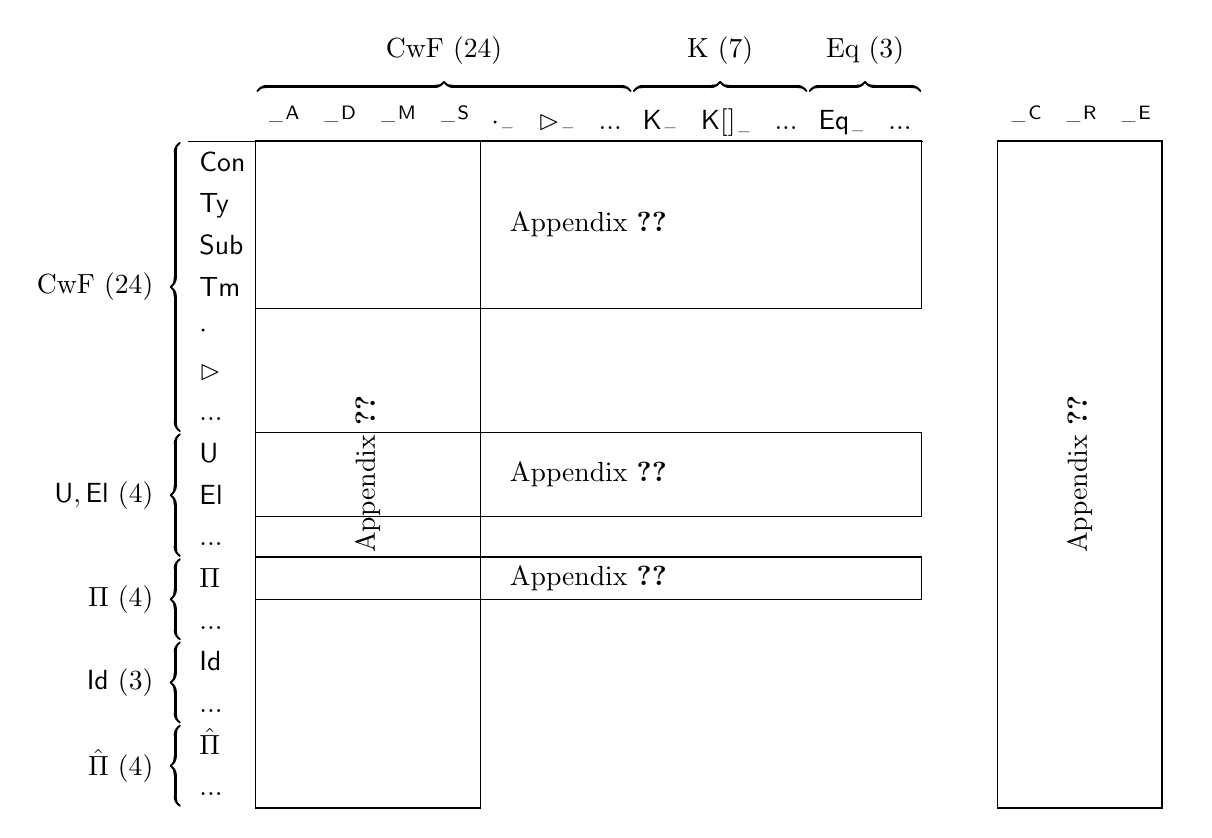
\begin{tikzpicture}[
node distance = 0pt,
    BC/.style = {
        decorate,
        decoration={calligraphic brace, amplitude=1.2mm,
        pre =moveto, pre  length=0.75pt,
        post=moveto, post length=0.75pt,
        raise=1mm,
        #1},% for mirroring of brace
        very thick,
        pen colour={black},
                  },
%  BC/.default = mirror,
    LN/.style = {inner xsep=4pt, outer sep=0pt},
                        ]
\matrix (m) [matrix of nodes, inner sep=0pt,
             nodes={text depth=0.8ex, text height=1em, %minimum width=5ex,
                    inner ysep=1pt, inner xsep=4pt, outer sep=0pt, anchor=west},
             nodes in empty cells,
             column sep=-\pgflinewidth,
             row sep= -\pgflinewidth,
             ]
{
             & $\blank^\A$   & $\blank^\D$    & $\blank^\M$  & $\blank^\S$  & $\cdot_{\blank}$ & $\rhd_{\blank}$ & ... & $\K_{\blank}$ & ${\K[]}_{\blank}$ & ... & $\Eq_{\blank}$  & ... & \hspace{2em} & $\blank^\C$ & $\blank^\R$ & $\blank^\E$ &  \\
    $\Con$   &              &                &              &              &                 &                &     &         &     &      &  &  &    &   & & &     \\
    $\Ty$    &              &                &              &              &                 &                &     &         &     &      &  &  &    &   & & &     \\
    $\Tms$   &              &                &              &              &                 &                &     &         &     &      &  &  &    &   & & &     \\
    $\Tm$    &              &                &              &              &                 &                &     &         &     &      &  &  &    &   & & &     \\
    $\cdot$  &              &                &              &              &                 &                &     &         &     &      &  &  &    &   & & &     \\
    $\rhd$   &              &                &              &              &                 &                &     &         &     &      &  &  &    &   & & &     \\
    $...$    &              &                &              &              &                 &                &     &         &     &      &  &  &    &   & & &     \\
    $\U$     &              &                &              &              &                 &                &     &         &     &      &  &  &    &   & & &     \\
    $\El$    &              &                &              &              &                 &                &     &         &     &      &  &  &    &   & & &     \\
    $...$    &              &                &              &              &                 &                &     &         &     &      &  &  &    &   & & &     \\
    $\Pi$    &              &                &              &              &                 &                &     &         &     &      &  &  &    &   & & &     \\
    $...$    &              &                &              &              &                 &                &     &         &     &      &  &  &    &   & & &     \\
    $\Id$    &              &                &              &              &                 &                &     &         &     &      &  &  &    &   & & &     \\
    $...$    &              &                &              &              &                 &                &     &         &     &      &  &  &    &   & & &     \\
    $\Pim$   &              &                &              &              &                 &                &     &         &     &      &  &  &    &   & & &     \\
    $...$    &              &                &              &              &                 &                &     &         &     &      &  &  &    &   & & &     \\
};
\draw           (m-1-1.south west) -- (m-1-13.south east);
\draw           (m-1-15.south west) -- (m-1-17.south east);

\draw (m-2-2.north west) rectangle (m-17-6.south west) node[pos=.5] {\rotatebox{90}{Appendix \ref{sec:app}}};

\draw (m-2-15.north west) rectangle (m-17-18.south west) node[pos=.5] {\rotatebox{90}{Appendix \ref{sec:app}}};

% \draw (m-2-2.north west) rectangle (m-17-3.south west) node[pos=.5] {\rotatebox{90}{Section \ref{sec:algebras}}};
% \draw (m-2-3.north west) rectangle (m-17-4.south west) node[pos=.5] {\rotatebox{90}{Section \ref{sec:eliminator}}};
% \draw (m-2-4.north west) rectangle (m-17-5.south west) node[pos=.5] {\rotatebox{90}{Section \ref{sec:recursor}}};
% \draw (m-2-5.north west) rectangle (m-17-6.south west) node[pos=.5] {\rotatebox{90}{Section \ref{sec:eliminator}}};

% \draw (m-2-15.north west) rectangle (m-17-16.south west) node[pos=.5] {\rotatebox{90}{Section \ref{sec:algebras}}};
% \draw (m-2-16.north west) rectangle (m-17-17.south west) node[pos=.5] {\rotatebox{90}{Section \ref{sec:recursor}}};
% \draw (m-2-17.north west) rectangle (m-17-18.south west) node[pos=.5] {\rotatebox{90}{Section \ref{sec:eliminator}}};

\draw (m-2-2.north west) rectangle (m-5-14.south west) node[pos=.5] {Appendix \ref{sec:motives}};

\draw (m-9-2.north west) rectangle (m-10-14.south west) node[pos=.5] {Appendix \ref{sec:motives}};
\draw (m-12-2.north west) rectangle (m-12-14.south west) node[pos=.5] {Appendix \ref{sec:motives}};

\draw[BC={},decoration={mirror}]    (m-2-1.north -| m.west) --
                    node[left=3mm] {CwF (24)}
                (m-8-1.south -| m.west);
\draw[BC={},decoration={mirror}]    (m-9-1.north -| m.west) --
                    node[left=3mm] {$\U,\El$ (4)}
                (m-11-1.south -| m.west);
\draw[BC={},decoration={mirror}]    (m-12-1.north -| m.west) --
                    node[left=3mm] {$\Pi$ (4)}
                (m-13-1.south -| m.west);
\draw[BC={},decoration={mirror}]    (m-14-1.north -| m.west) --
                    node[left=3mm] {$\Id$ (3)}
                (m-15-1.south -| m.west);
\draw[BC={},decoration={mirror}]    (m-16-1.north -| m.west) --
                    node[left=3mm] {$\Pim$ (4)}
                (m-17-1.south -| m.west);
%
\draw[BC]   let \p1 = ($(m-1-1.west)-(m-1-8.east)$),
                \n1 = {veclen(\x1,\y1)} in
            (m-1-2.north west) --
                node[text width=\n1, align=center,
                     above=3mm] {CwF (24)}
            (m-1-8.north east)
                    ;
\draw[BC]   let \p1 = ($(m-1-1.west)-(m-1-8.east)$),
                \n1 = {veclen(\x1,\y1)} in
            (m-1-9.north west) --
                node[text width=\n1, align=center,
                     above=3mm] {K (7)}
            (m-1-11.north east)
                    ;
\draw[BC]   let \p1 = ($(m-1-1.west)-(m-1-8.east)$),
                \n1 = {veclen(\x1,\y1)} in
            (m-1-12.north west) --
                node[text width=\n1, align=center,
                     above=3mm] {Eq (3)}
            (m-1-13.north east)
                    ;
% \draw[BC]   (m-8-7.south west) --
%                 node[align=center, below=3mm] {Expla- \\
%                                                nation}
%             (m-8-7.south east);
    \end{tikzpicture}
\]
}
\caption{The components in the CwF$^\K_{\Eq}$ model of the theory of
  signatures. We mark which components are listed in the appendices.}
\label{fig:table}
\end{figure}

There are two ways to present the model: by rows or by columns of the
table. Describing the model by rows is the usual way of saying how
contexts are given in the model, then how types are given, then
substitutions, terms, the empty context, context extension and so on.
Describing the model by columns means defining operations which
interpret the syntax, and later operations can depend on previous
ones. In Sections \ref{sec:algebras}--\ref{sec:eliminator} we used the
column-based method to describe the first four columns of this
table. These were given by $\blank^\A$, $\blank^\D$, $\blank^\M$, and
$\blank^\S$ (their full definition can be found in Appendix
\ref{sec:app}).

In this section we follow the row-based approach and describe the rows
of the model informally, while giving the full definition of the first
4 rows ($\Con$, $\Ty$, $\Tms$, $\Tm$) and the rows for $\U$, $\El$ and
$\Pi$ in Appendix \ref{sec:motives}. These are the most interesting
parts of the construction. The rest of the construction is tedious and
not very enlightening. The first 4 columns are fully formalised in
Agda and most parts of the category-columns from the CwF-columns are
also formalised.

The \textbf{CwF part} of the theory of signatures has to be
interpreted as the CwF of CwF$^\K_{\Eq}$s. Hence, $\Con$ is
interpreted as just CwF$^\K_{\Eq}$, while $\Sub$ is interpreted as the
set of strict CwF$^\K_{\Eq}$-morphisms (which strictly preserve all
structure), $\Ty$ is interpreted as the set of displayed
CwF$^\K_{\Eq}$s, and $\blank\rhd\blank$ is interpreted as the total
CwF$^\K_{\Eq}$ of a displayed one. Previously we illustrated how the
CwF of natural number algebras work in section
\ref{sec:cwfalg}. Constructing the CwF of CwF$^\K_{\Eq}$s is an
analogous, albeit much larger work. All in all, this part is a mostly
mechanical exercise.

For the \textbf{universe} $\U$ we have to give a concrete displayed
CwF$^\K_{\Eq}$, since $\U$ has type $\Ty\,\Gamma$, and we interpret
types as displayed CwF$^\K_{\Eq}$s.  However, $\U$ does not depend on
$\Gamma$, so we can give a non-displayed CwF$^\K_{\Eq}$, and then take
the constant displayed CwF$^\K_{\Eq}$ for that.

We interpret $\U$ as the CwF$^\K_{\Eq}$ of sets. It contains the
usual category of sets, and has families of sets and dependent
functions for families, function composition for substitution, and
extensional equality and constant families defined in the obvious way.
To see why this is the right choice, consider the one-element
signature containing just a $\U$. Since $\U^\A$ is $\Set$, the full
interpretation of this signature must be the CwF$^\K_{\Eq}$ of sets.

For interpreting \textbf{universe decoding} $\El\,a$, we have $a :
\Tm\,\Gamma\,\U$ and we need to construct a semantic $\Ty\,\Gamma$,
i.e. a displayed CwF$^\K_{\Eq}$. Here, $a$ is a CwF$^\K_{\Eq}$-section
of the interpretation of $\U$. However, we interpreted $\U$ as a
family which is constantly the CwF$^\K_{\Eq}$ of sets, so $a$ can be
viewed as a morphism from $\Gamma$ to the CwF$^\K_{\Eq}$ of
sets. Hence, we can define $\El\,a$ as the discrete
displayed CwF$^\K_{\Eq}$ where there are only identity morphisms.

When interpreting the \textbf{function space with small domain}, we
need to construct a $\Ty\,\Gamma$ from an $a : \Tm\,\Gamma\,\U$ and a
$B : \Ty\,(\Gamma\rhd\El\,a)$. The result has to internalise morphisms
from $a$ to $B$. We know that $(\Pi\,a\,B)^\A\,\gamma \equiv
(\alpha:a^\A\,\gamma)\ra B^\A\,(\gamma, \alpha)$, which has to be the
definition of the displayed objects in the result (a displayed object
is a dependent function), since $\blank^\A$ should yield this part of
the CwF$^\K_{\Eq}$ model. Note that $(\alpha:a^\A\,\gamma)\ra
B^\A\,(\gamma, \alpha)$ is just a plain function space, without any
conditions for functiorality or structure preservation. Fortunately,
we don't need such conditions because the domain $a$ is discrete. In
the implementation, all of the required displayed CwF$^\K_{\Eq}$
structure is inherited from the codomain; for example,
$\blank\rhd\blank$ is given by using the codomain's $\blank\rhd\blank$
pointwise, and $\pi_1$ is defined by postcomposing with the codomain's
$\pi_1$. The interpretation of $\APP$ generally follows the currying
pattern seen in $\APP^\A$.

The \textbf{function space with metatheoretic domain} is straightforward
to interpret. We have a metatheoretic $T : \Set$ and a function $B : T
\ra \Ty\,\Gamma$, and we need to create a semantic $\Ty\,\Gamma$. The
interpretation of $B$ is a function which returns a displayed
CwF$^\K_{\Eq}$, so it can be viewed as a function returning in a large
iterated $\Sigma$-type. We can just utilize the equivalence of
functions returning a $\Sigma$, and $\Sigma$s of functions, by pushing
the $T$ parameter inside the result components. In short, displayed
CwF$^\K_{\Eq}$s are closed under arbitrary direct products. Then,
$\app$ is interpreted as pointwise application of each component to a
metatheoretic argument.

For the \textbf{identity type}, we need to build a displayed
CwF$^\K_{\Eq}$ representing the equality of $t$ and $u$ sections of
some $a$ discrete displayed CwF$^\K_{\Eq}$. Because of the
discreteness, $a$ can be viewed as a morphism from a $\Gamma$
CwF$^\K_{\Eq}$ to the CwF$^\K_{\Eq}$ of sets, and $t$ and $u$ are
essentially sections of families of sets. Hence, we can define the
displayed objects in the result as pointwise equality of $t$ and $u$
(previously given in $\blank^\A$) and displayed displayed algebras as
pointwise equalities over equalities (previously given in
$\blank^\D$). Displayed morphisms, sections and all displayed
CwF$^\K_{\Eq}$ equations become trivial because of UIP. The
interpretation of equality reflection can be given using functional
extensionality.

This concludes the CwF$^\K_{\Eq}$ model of the theory of
signatures. Now, it follows that for each signature, there is a
CwF$^\K_{\Eq}$ of algebras, and thus induction is equivalent to
initiality by Section \ref{sec:initind}. Since for each signature we
have constructed an algebra with induction in Section
\ref{sec:algebras} and Section \ref{sec:eliminator}, it follows that
the constructed algebras are also initial.


%% %--------------------------------------------------------------------

\section{Conclusions and further work}
\label{sec:conclusions}

The present paper develops further the work in
\cite{kaposi_et_al:LIPIcs:2018:9190} where a syntax for HIITs was
presented but no construction for HIITs was given. In the present
paper we do construct initial algebras and (equivalently) eliminators,
although in a restricted setting: we only consider quotient
inductive-inductive types, and no higher equalities can be declared.

Note that the current theory of signatures is universal for closed
QIITs: this means that the theory of signatures without $\Pim$ can
describe its own signature. This perhaps opens the way for type
theories with \emph{levitated} QIIT codes in the style of
\cite{chapman2010gentle}. Also, the theory of closed QIIT signatures
can be viewed as a fragment of extensional type theory, hence this
part of our work can be viewed as a reduction of closed QIITs to the
existence of the syntax of extensional type theory.

Another limitation of the current work is that we only allow finitary
constructors, i.e. we do not internalise a rule for externally
indexed $\Pi$-types ($\Pii$). To obtain infinitary QIITs, we need to
add another $\Pi$-type:
\begin{alignat*}{5}
  & \Pii && : (T:\Set)\ra(T\ra\Tm\,\Gamma\,\U)\ra\Tm\,\Gamma\,\U %\\
\end{alignat*}
such that there is a natural isomorphism between
$\Tm\,\Gamma\,(\El\,(\Pii\,T\,b))$ and $(\alpha:T) \ra
\Tm\,\Gamma\,(\El\,(b\,\alpha))$.

Using the current definition, we are unable to interpret this type
former in the construction of initial algebras, because where we need
to derive a propositional equality, we only get an isomorphism. Since
our constructions rely on UIP, we cannot appeal to univalence to solve
this. Hence, we are unable to represent QIITs which are infinitely
branching such as W-types or the Cauchy reals \cite{HoTTbook}. A
potential solution would be to replace the propositional equalities in
the initial algebra construction (in the interpretation of terms and
substitutions) with isomorphisms in the CwF$^{\K}_{\Eq}$ of
algebras. We leave this for future work.

The restriction to QIITs instead of HIITs seems harder to overcome. In
any case, since homomorphisms of non-truncated algebras are generally
not homotopy sets, we would need to handle higher categories of
algebras in the semantics, which poses considerable technical
difficulty, and there is no known practical way to encode them in our
currently used metatheory (Martin-Löf type theory).

Also, there is a \emph{coherence} problem when interpreting the theory
signatures in a setting without UIP: in such a setting, we need to
set-truncate the syntax, but the metatheoretic universe is not a set,
hence we can't eliminate into it. This prevents us already from
defining the $\blank^\A$ operation, i.e. the standard model. If we
want to omit truncation, we need to add coherence laws, e.g. we need
to replace categories with $(\infty,1)$-categories, which could be
defined in a two-level type theory \cite{semisegal}, but it is not
clear in general what these coherences should be. However, if such a
higher syntax for signatures is possible, then perhaps the HIIT of
higher signatures would be universal for HIITs.


%%------------------------------------------------------------


%% Acknowledgments
\begin{acks}                            %% acks environment is optional
This work was supported by the European Union, co-financed by the
European Social Fund (EFOP-3.6.3-VEKOP-16-2017-00002) and COST Action
EUTypes CA15123.
\end{acks}


%% Bibliography
\bibliography{references}

%% Appendix
\appendix
\begin{landscape}
\section{Definitions of the operations from Sections \ref{sec:algebras}--\ref{sec:eliminator}}
\label{sec:app}

In this appendix we give the full definitions of the operations
$\blank^\A$, $\blank^\C$ (Section \ref{sec:algebras}), $\blank^\M$,
$\blank^\R$ (Section \ref{sec:recursor}), $\blank^\D$, $\blank^\S$,
$\blank^\E$ (Section \ref{sec:eliminator}).

{\footnotesize
\begin{alignat*}{10}
  & \text{\textbf{Syntax}}                                                                             && \rlap{$\text{\textbf{Algebras}}$} &&                                                      && \rlap{$\text{Assuming $\Omega:\Con$, the \textbf{initial $\Omega$-algebra} is given by $\con_\Omega:\equiv \Omega^\C\,\id$}$}                                                                                          \\
  & \Gamma:\Con                                                                                        && \Gamma^\A && : \Set                                                                             && \Gamma^\C && : \Tms\,\Omega\,\Gamma\ra\Gamma^\A                                                                                          \\
  & A:\Ty\,\Gamma                                                                                      && A^\A && : \Gamma^\A\ra\Set                                                                      && A^\C && : (\nu:\Tms\,\Omega\,\Gamma)\ra\Tm\,\Omega\,(A[\nu])\ra A^\A\,(\Gamma^\C\,\nu)                                                   \\
  & \sigma:\Tms\,\Gamma\,\Delta                                                                        && \sigma^\A && : \Gamma^\A\ra\Delta^\A                                                            && \sigma^\C && : (\nu:\Tms\,\Omega\,\Gamma)\ra \Delta^\C\,(\sigma\circ\nu)=\sigma^\A\,(\Gamma^\C\,\nu)                                     \\
  & t:\Tm\,\Gamma\,A                                                                                   && t^\A && : (\gamma:\Gamma^\A)\ra A^\A\,\gamma                                                    && t^\C && : (\nu:\Tms\,\Omega\,\Gamma)\ra A^\C\,\nu\,(t[\nu])=t^\A\,(\Gamma^\C\,\nu)                                                       \\
  & \cdot:\Con                                                                                         && \cdot^\A && :\equiv \top                                                                        && \cdot^\C\,\nu && :\equiv \tt                                                                                                             \\
  & \Gamma\rhd A:\Con                                                                                  && (\Gamma\rhd A)^\A && :\equiv (\gamma:\Gamma^\A)\times A^\A\,\gamma                              && (\Gamma\rhd A)^\C\,\nu && :\equiv (\Gamma^\C\,(\pi_1\,\nu),A^\C\,(\pi_1\,\nu)\,(\pi_2\,\nu))                                             \\
  & (A:\Ty\,\Delta)[\sigma:\Tms\,\Gamma\,\Delta]:\Ty\,\Gamma                                           && (A[\sigma])^\A\,\gamma && :\equiv A^\A\,(\sigma^\A\,\gamma)                                     && (A[\sigma])^\C\,\nu\,t && :\equiv \tr_{A^\A}\,(\sigma^\C\,\nu)\,(A^\C\,(\sigma\circ\nu)\,t)                                              \\
  & \id : \Tms\,\Gamma\,\Gamma                                                                         && \id^\A\,\gamma && :\equiv \gamma                                                                && \id^\C\,\nu && : \Gamma^\C\,\nu = \Gamma^\C\,\nu                                                                                                             \\
  & (\sigma:\Tms\,\Theta\,\Delta)\circ(\delta:\Tms\,\Gamma\,\Theta):\Tms\,\Gamma\,\Delta               && (\sigma\circ\delta)^\A\,\gamma && :\equiv \sigma^\A\,(\delta^\A\,\gamma)                        && (\sigma\circ\delta)^\C\,\nu && : \Delta^\C\,(\sigma\circ\delta\circ\nu) \overset{\sigma^\C\,(\delta\circ\nu)}{=} \sigma^\A\,(\Theta^\C\,(\delta\circ\nu)) \overset{\delta^\C\,\nu}{=} \sigma^\A\,(\delta^\A\,(\Gamma^\C\,\nu)) \\
  & \epsilon : \Tms\,\Gamma\,\cdot                                                                     && \epsilon^\A\,\gamma && :\equiv \tt                                                              && \epsilon^\C\,\nu && : \tt = \tt                                                                                                        \\
  & (\sigma:\Tms\,\Gamma\,\Delta) , (t:\Tm\,\Gamma\,(A[\sigma])):\Tms\,\Gamma\,(\Delta\rhd A)\hspace{1em}          && (\sigma, t)^\A\,\gamma && :\equiv (\sigma^\A\,\gamma, t^\A\,\gamma)                             && (\sigma,t)^\C\,\nu && : (\Gamma^\C\,(\sigma\circ\nu), A^\C\,(\sigma\circ\nu)\,(t[\nu])) \overset{\sigma^\C\,\nu, t^\C\,\nu}{=} (\sigma^\A\,(\Gamma^\C\,\nu), t^\A\,(\Gamma^\C\,\nu))                                                                        \\
  & \pi_1\,(\sigma:\Tms\,\Gamma\,(\Delta\rhd A)):\Tms\,\Gamma\,\Delta                                  && (\pi_1\,\sigma)^\A\,\gamma && :\equiv \proj_1\,(\sigma^\A\,\gamma)                              && (\pi_1\,\sigma)^\C\,\nu && : \Delta^\C\,(\pi_1\,(\sigma\circ\nu)) \overset{\sigma^\C\,\nu}{=} \proj_1\,(\sigma^\A\,(\Gamma^\C\,\nu))                                                                        \\
  & \pi_2\,(\sigma:\Tms\,\Gamma\,(\Delta\rhd A)):\Tm\,\Gamma\,(A[\pi_1\,\sigma])                       && (\pi_2\,\sigma)^\A\,\gamma && :\equiv \proj_2\,(\sigma^\A\,\gamma)                              && (\pi_2\,\sigma)^\C\,\nu && : A^\C\,(\pi_1\,(\sigma\circ\nu))\,(\pi_2\,(\sigma\circ\nu)) \overset{\sigma^\C\,\nu}{=} \proj_2\,(\sigma^\A\,(\Gamma^\C\,\nu))                                                                           \\
  & (t:\Tm\,\Delta\,A)[\sigma:\Tms\,\Gamma\,\Delta]:\Tm\,\Gamma\,(A[\sigma])                           && (t[\sigma])^\A\,\gamma && :\equiv t^\A\,(\sigma^\A\,\gamma)                                     && (t[\sigma])^\C\,\nu && : A^\C\,(\sigma\circ\nu)\,(t [\sigma\circ\nu]) \overset{t^\C(\sigma\circ\nu)}{=} t^\A\,(\delta^\C\,(\sigma\circ\nu))\overset{\sigma^\C\,\nu}{=}t^\A\,(\sigma^\A(\Gamma^\C\,\nu))  \\
  & [\id] : A[\id] = A                                                                                 && [\id]^\A && :\equiv \refl                                                                       && [\id]^\C && : A^\C\,\nu\,t = A^\C\,\nu\,t                                                                                                                \\
  & [\circ] : A[\sigma \circ \delta] = A[\sigma][\delta]                                               && [\circ]^\A && :\equiv \refl                                                                     && [\circ]^\C && : A^\C\,(\sigma\circ\delta\circ\nu)\,t = A^\C\,(\sigma\circ\delta\circ\nu)\,t                                                       \\
  & \ass : (\sigma \circ \delta) \circ \nu = \sigma \circ (\delta \circ \nu)                           && \ass^\A && :\equiv \refl                                                                        && \ass^\C && :\equiv \UIP                                                                                              \\
  & \idl : \id\circ\sigma = \sigma                                                                     && \idl^\A && :\equiv \refl                                                                        && \idl^\C && :\equiv \UIP                                                                                              \\
  & \idr : \sigma\circ\id = \sigma                                                                     && \idr^\A && :\equiv \refl                                                                        && \idr^\C && :\equiv \UIP                                                                                              \\
  & {\cdot\eta} : \{\sigma : \Tms\,\Gamma\,\cdot\} \ra \sigma = \epsilon                               && {\cdot\eta}^\A && :\equiv \refl                                                                 && {\cdot\eta}^\C && :\equiv \UIP                                                                                       \\
  & {\rhd\beta_1} : \pi_1\,(\sigma, t) = \sigma                                                        && {\rhd\beta_1}^\A && :\equiv \refl                                                               && {\rhd\beta_1}^\C&& :\equiv \UIP                                                                                      \\
  & {\rhd\beta_2} : \pi_2\,(\sigma, t) = t                                                             && {\rhd\beta_2}^\A && :\equiv \refl                                                               && {\rhd\beta_2}^\C && :\equiv \UIP                                                                                     \\
  & {\rhd\eta} : (\pi_1\,\sigma, \pi_2\,\sigma) = \sigma                                               && {\rhd\eta}^\A && :\equiv \refl                                                                  && {\rhd\eta}^\C&& :\equiv \UIP                                                                                         \\
  & {,\circ} : (\sigma, t)\circ\delta = (\sigma\circ\delta, t[\delta])                                 && {,\circ}^\A && :\equiv \refl                                                                    && {,\circ}^\C && :\equiv \UIP                                                                                          \\
  & \U : \Ty\,\Gamma                                                                                   && \U^\A\,\gamma && :\equiv \Set                                                                   && \U^\C\,\nu\,a && :\equiv \Tm\,\Omega\,(\El\,a)                                                                                        \\
  & \El\,(a: \Tm\,\Gamma\,\U): \Ty\,\Gamma                                                             && (\El\,a)^\A\,\gamma && :\equiv a^\A\,\gamma                                                     && (\El\,a)^\C\,\nu\,t    && :\equiv \coe\,(a^\C\,\nu : \Tm\,\Omega\,(\El\,a)=a^\A\,(\Gamma^\C\,\nu))\,t                                                                                   \\
  & {\U[]} : \U[\sigma] = \U                                                                           && {\U[]}^\A && :\equiv \refl                                                                      && {\U[]}^\C && : \Tm\,\Omega\,a=\Tm\,\Omega\,a                                                  \\
  & {\El[]} : (\El\,a)[\sigma] = \El\,(a[\sigma])                                                      && {\El[]}^\A && :\equiv \refl                                                                     && {\El[]}^\C && : t = t                                                                                        \\
  & \Pi\,(a:\Tm\,\Gamma\,\U)(B:\Ty\,(\Gamma\rhd\El\,a)):\Ty\,\Gamma                                    && (\Pi\,a\,B)^\A\,\gamma && :\equiv (\alpha:a^\A\,\gamma)\ra B^\A\,(\gamma, \alpha) \hspace{1em}  && (\Pi\,a\,B)^\C\,\nu\,t && :\equiv \lambda\alpha.B^\C\,(\nu,\coe\,({a^\C\,\nu^{-1}})\,\alpha)\,(t\app \coe\,({a^\C\,\nu^{-1}})\,\alpha)   \\
  & \APP\,(t:\Tm\,\Gamma\,(\Pi\,a\,B)):\Tm\,(\Gamma\rhd\El\,a)\,B\hspace{1em}                          && (\APP\,t)^\A\,(\gamma,\alpha) && :\equiv t^\A\,\gamma\,\alpha                                    && (\APP\,t)^\C\,\nu    && : B^\C\,\nu\,((\APP\,t)[\nu]) \overset{t^\C\,(\pi_1\,\nu)}{=} t^\A\,(\Gamma^\C\,(\pi_1\,\nu))\,(\pi_2\,\nu)                                                                                                          \\
  & {\Pi[]} : (\Pi\,a\,B)[\sigma] = \Pi\,(a[\sigma])\,(B[\sigma^\uparrow])                              && {\Pi[]}^\A && :\equiv \refl                                                                    &&  {\Pi[]}^\C && : \lambda\alpha.B^\C\,(\sigma\circ\nu,\alpha)\,(t\app\alpha) = \lambda\alpha.B^\C\,(\sigma\circ\nu,\alpha)\,(t\app\alpha)                                                                                                                   \\
  & {\APP[]} : (\APP\,t)[\sigma\uparrow] = \APP\,(t[\sigma])                                           && {\APP[]}^\A && :\equiv \refl                                                                    && {\APP[]}^\C && :\equiv \UIP                                                                                          \\
  & \Id\,(a:\Tm\,\Gamma\,\U)\,(t\,u:\Tm\,\Gamma\,(\El\,a)):\Ty\,\Gamma                                 && (\Id\,a\,t\,u)^\A\,\gamma && :\equiv (t^\A\,\gamma=u^\A\,\gamma)                                && (\Id\,a\,t\,u)^\C\,\nu\,e && : t^\A\,(\Gamma^\C\,\nu)\overset{t^\C\,\nu}{=} t[\nu] \overset{\reflect\,e}{=} u[\nu] \overset{u^\C\,\nu}{=} u^\A\,(\Gamma^\C\,\nu)                                                                                                    \\
  & \reflect\,(e:\Tm\,\Gamma\,(\Id\,a\,t\,u)): t = u                                                   && (\reflect\,e)^\A && :\equiv \funext\,e^\A                                                       && (\reflect\,e)^\C && :\equiv \UIP                                                                                                              \\
  & {\Id[]} : (\Id\,a\,t\,u)[\sigma] = \Id\,(a[\sigma])\,(t[\sigma])\,(u[\sigma])                      && {\Id[]}^\A && :\equiv \refl                                                                     && {\Id[]}^\C && :\equiv \UIP                                                                                                                    \\
  & \Pim\,(T:\Set)\,(B:T\ra\Ty\,\Gamma):\Ty\,\Gamma                                                    && (\Pim\,T\,B)^\A\,\gamma && :\equiv (\alpha:T)\ra (B\,\alpha)^\A\,\gamma                         && (\Pim\,T\,B)^\C\,\nu\,t && :\equiv \lambda\alpha.(B\,\alpha)^\C\,\nu\,(t\appm\alpha)                                                                                                      \\
  & (t:\Tm\,\Gamma\,(\Pim\,T\,B))\appm(\alpha:T):\Tm\,\Gamma\,(B\,\alpha)                              && (t\appm\alpha)^\A\,\gamma && :\equiv t^\A\,\gamma\,\alpha                                       && (t\appm\alpha)^\C\,\nu    && : (B\,\alpha)^\C\,\nu\,(t[\nu]\appm\alpha)\overset{t^\C\,\nu}{=}t^\A\,(\Gamma^\C\,\nu)\,\alpha                                                                                                      \\
  & {\Pim[]} : (\Pim\,T\,B)[\sigma] = \Pim\,T\,(\lambda \alpha.(B\,\alpha)[\sigma])                    && {\Pim[]}^\A && :\equiv \refl                                                                    && {\Pim[]}^\C && : \lambda\alpha.(B\,\alpha)^\C\,(\sigma\circ\nu)\,(t\appm\alpha) =                                                                                                                    \\
  & && && && && \hspace{1.5em} \lambda\alpha.(B\,\alpha)^\C\,(\sigma\circ\nu)\,(t\appm\alpha)(\Pim\,T\,(\lambda\alpha.(B\,\alpha)[\sigma]))^\C\,\nu\,t                                                                                                                   \\
  & {\appm[]} : (t\appm\alpha)[\sigma] = (t[\sigma])\mathop{\appm}\alpha                               && {\appm[]}^\A && :\equiv \refl                                                                   && {\appm[]}^\C && :\equiv \UIP
\end{alignat*}

\newpage

\begin{alignat*}{10}
  & \text{\textbf{Syntax}}                                                                                && \rlap{$\text{\textbf{Homomorphisms}}$} &&                                                                                                                                       \\
  & \Gamma:\Con                                                                                           && \Gamma^\M && : \Gamma^\A\ra\Gamma^\A\ra\Set                                                                                                                                     \\
  & A:\Ty\,\Gamma                                                                                         && A^\M && : \Gamma^\M\,\gamma^\0\,\gamma^\1\ra A^\A\,\gamma^\0\ra A^\A\,\gamma^\1\Set                                                                                             \\
  & \sigma:\Tms\,\Gamma\,\Delta                                                                           && \sigma^\M && : \Gamma^\M\,\gamma^\0\,\gamma^\1\ra\Delta^\M\,(\sigma^\A\,\gamma^\0)\,(\sigma^\A\,\gamma^\1)                                                                      \\
  & t:\Tm\,\Gamma\,A                                                                                      && t^\M && : (\gamma^M:\Gamma^\M\,\gamma^\0\,\gamma^\1)\ra A^\M\,\gamma^M\,(t^\A\,\gamma^\0)\,(t^\A\,\gamma^\1)                                                                     \\
  & \cdot:\Con                                                                                            && \cdot^\M\,\tt\,\tt && :\equiv \top                                                                                                                                              \\
  & \Gamma\rhd A:\Con                                                                                     && (\Gamma\rhd A)^\M\,(\gamma^\0,\alpha^\0)\,(\gamma^\1,\alpha^\1) && :\equiv (\gamma^M:\Gamma^\M\,\gamma^\0\,\gamma^\1)\times A^\M\,\gamma^M\,\alpha^\0\,\alpha^\1                \\
  & (A:\Ty\,\Delta)[\sigma:\Tms\,\Gamma\,\Delta]:\Ty\,\Gamma                                              && (A[\sigma])^\M\,\gamma^M\,\alpha^\0\,\alpha^\1 && :\equiv A^\M\,(\sigma^\M\,\gamma^M)\,\alpha^\0\,\alpha^\1                                                                     \\
  & \id : \Tms\,\Gamma\,\Gamma                                                                            && \id^\M\,\gamma^M && :\equiv \gamma^m                                                                                                                                            \\
  & (\sigma:\Tms\,\Theta\,\Delta)\circ(\delta:\Tms\,\Gamma\,\Theta):\Tms\,\Gamma\,\Delta                  && (\sigma\circ\delta)^\M\,\gamma^M && :\equiv \sigma^\M\,(\delta^\M\,\gamma^M)                                                                                                    \\
  & \epsilon : \Tms\,\Gamma\,\cdot                                                                        && \epsilon^\M\,\gamma^M && :\equiv \tt                                                                                                                                            \\
  & (\sigma:\Tms\,\Gamma\,\Delta) , (t:\Tm\,\Gamma\,(A[\sigma])):\Tms\,\Gamma\,(\Delta\rhd A)\hspace{1em} && (\sigma, t)^\M\,\gamma^M && :\equiv (\sigma^\M\,\gamma^M, t^\M\,\gamma^M)                                                                                                       \\
  & \pi_1\,(\sigma:\Tms\,\Gamma\,(\Delta\rhd A)):\Tms\,\Gamma\,\Delta                                     && (\pi_1\,\sigma)^\M\,\gamma^M && :\equiv \proj_1\,(\sigma^\M\,\gamma^M)                                                                                                          \\
  & \pi_2\,(\sigma:\Tms\,\Gamma\,(\Delta\rhd A)):\Tm\,\Gamma\,(A[\pi_1\,\sigma])                          && (\pi_2\,\sigma)^\M\,\gamma^M && :\equiv \proj_2\,(\sigma^\M\,\gamma^M)                                                                                                          \\
  & (t:\Tm\,\Delta\,A)[\sigma:\Tms\,\Gamma\,\Delta]:\Tm\,\Gamma\,(A[\sigma])                              && (t[\sigma])^\M\,\gamma^M && :\equiv t^\M\,(\sigma^\M\,\gamma^M)                                                                                                                 \\
  & [\id] : A[\id] = A                                                                                    && [\id]^\M && :\equiv \refl                                                                                                                                                       \\
  & [\circ] : A[\sigma \circ \delta] = A[\sigma][\delta]                                                  && [\circ]^\M && :\equiv \refl                                                                                                                                                     \\
  & \ass : (\sigma \circ \delta) \circ \nu = \sigma \circ (\delta \circ \nu)                              && \ass^\M && :\equiv \refl                                                                                                                                                        \\
  & \idl : \id\circ\sigma = \sigma                                                                        && \idl^\M && :\equiv \refl                                                                                                                                                        \\
  & \idr : \sigma\circ\id = \sigma                                                                        && \idr^\M && :\equiv \refl                                                                                                                                                        \\
  & {\cdot\eta} : \{\sigma : \Tms\,\Gamma\,\cdot\} \ra \sigma = \epsilon                                  && {\cdot\eta}^\M && :\equiv \refl                                                                                                                                                 \\
  & {\rhd\beta_1} : \pi_1\,(\sigma, t) = \sigma                                                           && {\rhd\beta_1}^\M && :\equiv \refl                                                                                                                                               \\
  & {\rhd\beta_2} : \pi_2\,(\sigma, t) = t                                                                && {\rhd\beta_2}^\M && :\equiv \refl                                                                                                                                               \\
  & {\rhd\eta} : (\pi_1\,\sigma, \pi_2\,\sigma) = \sigma                                                  && {\rhd\eta}^\M && :\equiv \refl                                                                                                                                                  \\
  & {,\circ} : (\sigma, t)\circ\delta = (\sigma\circ\delta, t[\delta])                                    && {,\circ}^\M && :\equiv \refl                                                                                                                                                    \\
  & \U : \Ty\,\Gamma                                                                                      && \U^\M\,\gamma^M\,T^\0\,T^\1 && :\equiv T^\0\ra T^\1                                                                                                                             \\
  & \El\,(a: \Tm\,\Gamma\,\U): \Ty\,\Gamma                                                                && (\El\,a)^\M\,\gamma^M\,\alpha^\0\,\alpha^\1 && :\equiv a^\M\,\gamma^M\,\alpha^\0 = \alpha^\1                                                                                    \\
  & {\U[]} : \U[\sigma] = \U                                                                              && {\U[]}^\M && :\equiv \refl                                                                                                                                                      \\
  & {\El[]} : (\El\,a)[\sigma] = \El\,(a[\sigma])                                                         && {\El[]}^\M && :\equiv \refl                                                                                                                                                     \\
  & \Pi\,(a:\Tm\,\Gamma\,\U)(B:\Ty\,(\Gamma\rhd\El\,a)):\Ty\,\Gamma                                       && (\Pi\,a\,B)^\M\,\gamma^M\,f^\0\,f^\1 && :\equiv (\alpha^\0:a^\A\,\gamma^\0)\ra B^\M\,(\gamma^M, \refl)\,(f^\0\,\alpha^\0)\,(f^\1\,(a^\M\,\gamma^M\,\alpha^\0)) \hspace{1em}      \\
  & \APP\,(t:\Tm\,\Gamma\,(\Pi\,a\,B)):\Tm\,(\Gamma\rhd\El\,a)\,B\hspace{1em}                             && (\APP\,t)^\M\,(\gamma^M,\alpha^M) && :\equiv \J\,(t^\M\,\gamma^M\,\alpha^\0)\,\alpha^M                                                                                          \\
  & {\Pi[]} : (\Pi\,a\,B)[\sigma] = \Pi\,(a[\sigma])\,(B[\sigma^\uparrow])                                && {\Pi[]}^\M && :\equiv \refl                                                                                                                                                     \\
  & {\APP[]} : (\APP\,t)[\sigma\uparrow] = \APP\,(t[\sigma])                                              && {\APP[]}^\M && :\equiv \refl                                                                                                                                                    \\
  & \Id\,(a:\Tm\,\Gamma\,\U)\,(t\,u:\Tm\,\Gamma\,(\El\,a)):\Ty\,\Gamma                                    && (\Id\,a\,t\,u)^\M\,\gamma^M\,e^\0\,e^\1 && :\equiv\top                                                                                                                          \\
  & \reflect\,(e:\Tm\,\Gamma\,(\Id\,a\,t\,u)): t = u                                                      && (\reflect\,e)^\M && :\equiv \UIP                                                                                                                                                \\
  & {\Id[]} : (\Id\,a\,t\,u)[\sigma] = \Id\,(a[\sigma])\,(t[\sigma])\,(u[\sigma])                         && {\Id[]}^\M && :\equiv \refl                                                                                                                                                     \\
  & \Pim\,(T:\Set)\,(B:T\ra\Ty\,\Gamma):\Ty\,\Gamma                                                       && (\Pim\,T\,B)^\M\,\gamma^M\,f^\0\,f^\1 && :\equiv (\alpha:T)\ra (B\,\alpha)^\M\,\gamma^M\,(f^\0\,\alpha)\,(f^\1\,\alpha)                                                         \\
  & (t:\Tm\,\Gamma\,(\Pim\,T\,B))\appm(\alpha:T):\Tm\,\Gamma\,(B\,\alpha)                                 && (t\appm\alpha)^\M\,\gamma^M && :\equiv t^\M\,\gamma^M\,\alpha                                                                                                                  \\
  & {\Pim[]} : (\Pim\,T\,B)[\sigma] = \Pim\,T\,(\lambda \alpha.(B\,\alpha)[\sigma])                       && {\Pim[]}^\M && :\equiv \refl                                                                                                                                                   \\
  & {\appm[]} : (t\appm\alpha)[\sigma] = (t[\sigma])\mathop{\appm}\alpha                                  && {\appm[]}^\M && :\equiv \refl
\end{alignat*}

\newpage

\begin{alignat*}{10}
  & \text{\textbf{Syntax}}                                                                                && \rlap{$\text{Assuming $\omega:\Omega^\A$, the \textbf{recursor} is given by $\rec_\Omega\,\omega:\equiv \Omega^\R\,\id$}$}                                                                                          \\
  & \Gamma:\Con                                                                                           && \Gamma^\R && :(\nu:\Tms\,\Omega\,\Gamma)\ra \Gamma^\R\,(\nu^\A\,\con)\,(\nu^\A\,\omega)                              \\
  & A:\Ty\,\Gamma                                                                                         && A^\R && :(\nu:\Tms\,\Omega\,\Gamma)(t:\Tm\,\Omega\,(A[\nu]))\ra A^\M\,(\Gamma^\R\,\nu)\,(t^\A\,\con)\,(t^\A\,\omega) \\
  & \sigma:\Tms\,\Gamma\,\Delta                                                                           && \sigma^\R && :(\nu:\Tms\,\Omega\,\Gamma)\ra \Delta^\R\,(\sigma\circ\nu) = \sigma^\M\,(\Gamma^\R\,\nu)                \\
  & t:\Tm\,\Gamma\,A                                                                                      && t^\R && :(\nu:\Tms\,\Omega\,\Gamma)\ra A^\R\,\nu\,(t[\nu]) = t^\M\,(\Gamma^\R\,\nu)                                  \\
  & \cdot:\Con                                                                                            && \cdot^\R\,\nu && :\equiv \tt                                                                                         \\
  & \Gamma\rhd A:\Con                                                                                     && (\Gamma\rhd A)^\R\,\nu && :\equiv \big(\Gamma^\R\,(\pi_1\,\nu), A^\R\,(\pi_1\,\nu)\,(\pi_2\,\nu)\big)                \\
  & (A:\Ty\,\Delta)[\sigma:\Tms\,\Gamma\,\Delta]:\Ty\,\Gamma                                              && (A[\sigma])^\R\,\nu\,t && :\equiv \tr_{(A^\M\,\blank\,(t^\A\,\con)\,(t^\A\,\omega))}\,(\sigma^\R\,\nu)\,(A^\R\,(\sigma\circ\nu)\,t)                           \\
  & \id : \Tms\,\Gamma\,\Gamma                                                                            && \id^\R\,\nu && :\Gamma^\R\,\nu = \Gamma^\E\,\nu                                                                                                        \\
  & (\sigma:\Tms\,\Theta\,\Delta)\circ(\delta:\Tms\,\Gamma\,\Theta):\Tms\,\Gamma\,\Delta                  && (\sigma\circ\delta)^\R\,\nu && : \Delta^\R\,(\sigma\circ\delta\circ\nu) \overset{\sigma^\R\,(\delta\circ\nu)}{=} \sigma^\M\,(\Theta^\R\,(\delta\circ\nu)) \overset{\delta^\R\,\nu}{=} \sigma^\M\,(\delta^\M\,(\Gamma^\R\,\nu))                                      \\
  & \epsilon : \Tms\,\Gamma\,\cdot                                                                        && \epsilon^\R\,\nu && : \tt = \tt                                                                                                                                    \\
  & (\sigma:\Tms\,\Gamma\,\Delta) , (t:\Tm\,\Gamma\,(A[\sigma])):\Tms\,\Gamma\,(\Delta\rhd A)\hspace{1em} && (\sigma,t)^\R\,\nu && : (\Delta^\R\,(\sigma\circ\nu),A^\R\,(\sigma\circ\nu)\,(t[\nu])) \overset{\sigma^\R\,\nu, t^\R\,\nu}{=} (\sigma^\M\,(\Gamma^\R\,\nu), t^\M\,(\Gamma^\R\,\nu))                                      \\
  & \pi_1\,(\sigma:\Tms\,\Gamma\,(\Delta\rhd A)):\Tms\,\Gamma\,\Delta                                     && (\pi_1\,\sigma)^\R\,\nu && : \proj_1\,((\Delta\rhd A)^\R\,(\sigma\circ\nu)) \overset{\sigma^\R\,\nu}{=} \proj_1\,(\sigma^\M\,(\Gamma^\R\,\nu))                                      \\
  & \pi_2\,(\sigma:\Tms\,\Gamma\,(\Delta\rhd A)):\Tm\,\Gamma\,(A[\pi_1\,\sigma])                          && (\pi_2\,\sigma)^\R\,\nu && : \proj_2\,((\Delta\rhd A)^\R\,(\sigma\circ\nu)) \overset{\sigma^\R\,\nu}{=} \proj_2\,(\sigma^\M\,(\Gamma^\R\,\nu))                                      \\
  & (t:\Tm\,\Delta\,A)[\sigma:\Tms\,\Gamma\,\Delta]:\Tm\,\Gamma\,(A[\sigma])                              && (t[\sigma])^\R\,\nu && : A^\R\,(\sigma\circ\nu)\,(t[\sigma][\nu]) \overset{t^\R\,(\sigma\circ\nu)}{=} t^\M\,(\Delta^\R\,(\sigma\circ\nu)) \overset{\sigma^\R\,\nu}{=} t^\M\,(\sigma^\M\,(\Gamma^\R\,\nu))                                      \\
  & [\id] : A[\id] = A                                                                                    && [\id]^\R && : A^\R\,\nu\,t = A^\R\,\nu\,t                                      \\
  & [\circ] : A[\sigma \circ \delta] = A[\sigma][\delta]                                                  && [\circ]^\R && : A^\R\,(\sigma\circ\delta\circ\nu)\,t = A^\R\,(\sigma\circ\delta\circ\nu)\,t \\
  & \ass : (\sigma \circ \delta) \circ \nu = \sigma \circ (\delta \circ \nu)                              && \ass^\R && :\equiv \UIP                                                  \\
  & \idl : \id\circ\sigma = \sigma                                                                        && \idl^\R && :\equiv \UIP                                                  \\
  & \idr : \sigma\circ\id = \sigma                                                                        && \idr^\R && :\equiv \UIP                                                  \\
  & {\cdot\eta} : \{\sigma : \Tms\,\Gamma\,\cdot\} \ra \sigma = \epsilon                                  && {\cdot\eta}^\R && :\equiv \UIP                                           \\
  & {\rhd\beta_1} : \pi_1\,(\sigma, t) = \sigma                                                           && {\rhd\beta_1}^\R && :\equiv \UIP                                          \\
  & {\rhd\beta_2} : \pi_2\,(\sigma, t) = t                                                                && {\rhd\beta_2}^\R && :\equiv \UIP                                         \\
  & {\rhd\eta} : (\pi_1\,\sigma, \pi_2\,\sigma) = \sigma                                                  && {\rhd\eta}^\R && :\equiv \UIP                                             \\
  & {,\circ} : (\sigma, t)\circ\delta = (\sigma\circ\delta, t[\delta])                                    && {,\circ}^\R && :\equiv \UIP                                              \\
  & \U : \Ty\,\Gamma                                                                                      && \U^\R\,\nu\,a && :\equiv \lambda \alpha.\big(\coe\,({a^\C\,\id}^{-1})\,\alpha\big)^\A\,\omega                                     \\
  & \El\,(a: \Tm\,\Gamma\,\U): \Ty\,\Gamma                                                                && (\El\,a)^\R\,\nu\,t && : a^\M\,(\Gamma^\R\,\nu)\,(t^\A\,\con)\overset{t^\C\,\id}{=}a^\M\,(\Gamma^\R\,\nu)\,t \overset{a^\R\,\nu}{=}t^\A\,\omega                                      \\
  & {\U[]} : \U[\sigma] = \U                                                                              && {\U[]}^\R && : \alpha.\alpha^\A\,\omega = \alpha.\alpha^\A\,\omega                                      \\
  & {\El[]} : (\El\,a)[\sigma] = \El\,(a[\sigma])                                                         && {\El[]}^\R && :\equiv \UIP                                      \\
  & \Pi\,(a:\Tm\,\Gamma\,\U)(B:\Ty\,(\Gamma\rhd\El\,a)):\Ty\,\Gamma                                       && (\Pi\,a\,B)^\R\,\nu\,t && :\equiv \lambda\alpha.\LET\,u:\equiv \coe\,({a^\C\,\nu}^{-1})\,(\tr_{a^\A}\,({\nu^\C\,\id}^{-1}) \alpha) \,\IN \,\tr\,({u^\C\,\id}^{-1})\,\big(\tr\,(a^\R\,\nu)\,(B^\R\,(\nu,u)\,(t\app u))\big) \\
  & \APP\,(t:\Tm\,\Gamma\,(\Pi\,a\,B)):\Tm\,(\Gamma\rhd\El\,a)\,B\hspace{1em}                             && (\APP\,t)^\R\,(\nu, u) && : B^\R\,(\nu,u)\,(t[\nu]\app u) \overset{t^\R\,\nu}{=} t^\M\,(\Gamma^\R\,\nu)                                      \\
  & {\Pi[]} : (\Pi\,a\,B)[\sigma] = \Pi\,(a[\sigma])\,(B[\sigma^\uparrow])                                && {\Pi[]}^\R && : \lambda\alpha.B^\R\,(\sigma\circ\nu,\alpha)\,(t\app\alpha) = \lambda\alpha.B^\R\,(\sigma\circ\nu,\alpha)\,(t\app\alpha)  \\
  & {\APP[]} : (\APP\,t)[\sigma\uparrow] = \APP\,(t[\sigma])                                              && {\APP[]}^\R && :\equiv \UIP                                      \\
  & \Id\,(a:\Tm\,\Gamma\,\U)\,(t\,u:\Tm\,\Gamma\,(\El\,a)):\Ty\,\Gamma                                    && {\Id\,a\,t\,u}^\R\,\nu\,e && :\equiv \tt                                      \\
  & \reflect\,(e:\Tm\,\Gamma\,(\Id\,a\,t\,u)): t = u                                                      && (\reflect\,e)^\R && :\equiv \UIP                                      \\
  & {\Id[]} : (\Id\,a\,t\,u)[\sigma] = \Id\,(a[\sigma])\,(t[\sigma])\,(u[\sigma])                         && {\Id[]}^\R && : \tt = \tt                                      \\
  & \Pim\,(T:\Set)\,(B:T\ra\Ty\,\Gamma):\Ty\,\Gamma                                                       && (\Pim\,T\,B)^\R\,\nu\,t && :\equiv \lambda\alpha.(B\,\alpha)^\R\,\nu\,(t\appm\alpha)                                     \\
  & (t:\Tm\,\Gamma\,(\Pim\,T\,B))\appm(\alpha:T):\Tm\,\Gamma\,(B\,\alpha)                                 && (t\appm\alpha)^\R\,\nu && : (B\,\alpha)^\R\,\nu\,(t[\nu]\appm\alpha) \overset{t^\R\,\nu}{=} t^\M\,(\Gamma^\R\,\nu)\,\alpha                                      \\
  & {\Pim[]} : (\Pim\,T\,B)[\sigma] = \Pim\,T\,(\lambda \alpha.(B\,\alpha)[\sigma])                       && {\Pim[]}^\R && : \lambda\alpha.(B\,\alpha)^\R\,(\sigma\circ\nu)\,(t\appm\alpha) = \lambda\alpha.(B\,\alpha)^\R\,(\sigma\circ\nu)\,(t\appm\alpha)                              \\
  & {\appm[]} : (t\appm\alpha)[\sigma] = (t[\sigma])\mathop{\appm}\alpha                                  && {\appm[]}^\R && :\equiv \UIP
\end{alignat*}

\newpage

\begin{alignat*}{10}
  & \text{\textbf{Syntax}}                                                                                      && \rlap{$\text{\textbf{Displayed algebras}}$} &&                                                                                                                    && \rlap{$\text{\textbf{Sections}}$}                                                                                                                                              \\
  & \Gamma:\Con                                                                                        && \Gamma^\D && : \Gamma^\A\ra\Set                                                                                                                && \Gamma^\S && : (\gamma:\Gamma^\A)\ra\Gamma^\D\,\gamma\ra\Set                                                                                                          \\
  & A:\Ty\,\Gamma                                                                                      && A^\D && : \Gamma^\D\,\gamma\ra A^\A\,\gamma\ra\Set                                                                                             && A^\S && : \Gamma^\S\,\gamma\,\gamma^D\ra (\alpha:A^\A\,\gamma)\ra A^\D\,\gamma^D\,\alpha\ra\Set                                                                       \\
  & \sigma:\Tms\,\Gamma\,\Delta                                                                        && \sigma^\D && : \Gamma^\D\,\gamma\ra\Delta^\D\,(\sigma^\A\,\gamma)                                                                              && \sigma^\S && : \Gamma^\S\,\gamma\,\gamma^D\ra\Delta^\S\,(\sigma^\A\,\gamma)\,(\sigma^\D\,\gamma^D)                                                                    \\
  & t:\Tm\,\Gamma\,A                                                                                   && t^\D && : (\gamma^D:\Gamma^\D\,\gamma)\ra A^\D\,\gamma^D\,(t^\A\,\gamma)                                                                       && t^\S && : (\gamma^S:\Gamma^\S\,\gamma\,\gamma^D)\ra A^\S\,\gamma^S\,(t^\A\,\gamma)\,(t^\D\,\gamma^D)                                                                  \\
  & \cdot:\Con                                                                                         && \cdot^\D\,\tt && :\equiv \top                                                                                                                  && \cdot^\S\,\tt\,\tt && :\equiv \top                                                                                                                                    \\
  & \Gamma\rhd A:\Con                                                                                  && (\Gamma\rhd A)^\D\,(\gamma, \alpha) && :\equiv (\gamma^D:\Gamma^\D\,\gamma)\times A^\D\,\gamma^D\,\alpha                                       && (\Gamma\rhd A)^\S\,(\gamma, \alpha)\,(\gamma^D, \alpha^D) && :\equiv (\gamma^S:\Gamma^\S\,\gamma\,\gamma^D)\times A^\S\,\gamma^S\,\alpha\,\alpha^D                    \\
  & (A:\Ty\,\Delta)[\sigma:\Tms\,\Gamma\,\Delta]:\Ty\,\Gamma                                           && (A[\sigma])^\D\,\gamma^D\,\alpha && :\equiv A^\D\,(\sigma^\D\,\gamma^D)\,\alpha                                                                && (A[\sigma])^\S\,\gamma^S\,\alpha\,\alpha^D && :\equiv A^\S\,(\sigma^\S\,\gamma^S)\,\alpha\,\alpha^D                                                                   \\
  & \id : \Tms\,\Gamma\,\Gamma                                                                         && \id^\D\,\gamma^D && :\equiv \gamma^D                                                                                                           && \id^\S\,\gamma^S && :\equiv \gamma^S                                                                                                                                  \\
  & (\sigma:\Tms\,\Theta\,\Delta)\circ(\delta:\Tms\,\Gamma\,\Theta):\Tms\,\Gamma\,\Delta               && (\sigma\circ\delta)^\D\,\gamma^D && :\equiv \sigma^\D\,(\delta^\D\,\gamma^D)                                                                   && (\sigma\circ\delta)^\S\,\gamma^S && :\equiv \sigma^\S\,(\delta^\S\,\gamma^S)                                                                                          \\
  & \epsilon : \Tms\,\Gamma\,\cdot                                                                     && \epsilon^\D\,\gamma^D && :\equiv \tt                                                                                                           && \epsilon^\S\,\gamma^S && :\equiv \tt                                                                                                                                  \\
  & (\sigma:\Tms\,\Gamma\,\Delta) , (t:\Tm\,\Gamma\,(A[\sigma])):\Tms\,\Gamma\,(\Delta\rhd A)\hspace{1em} && (\sigma, t)^\D\,\gamma^D && :\equiv (\sigma^\D\,\gamma^D, t^\D\,\gamma^D)                                                                      && (\sigma, t)^\S\,\gamma^S && :\equiv (\sigma^\S\,\gamma^S, t^\S\,\gamma^S)                                                                                             \\
  & \pi_1\,(\sigma:\Tms\,\Gamma\,(\Delta\rhd A)):\Tms\,\Gamma\,\Delta                                  && (\pi_1\,\sigma)^\D\,\gamma^D && :\equiv \proj_1\,(\sigma^\D\,\gamma^D)                                                                         && (\pi_1\,\sigma)^\S\,\gamma^S && :\equiv \proj_1\,(\sigma^\S\,\gamma^S)                                                                                                \\
  & \pi_2\,(\sigma:\Tms\,\Gamma\,(\Delta\rhd A)):\Tm\,\Gamma\,(A[\pi_1\,\sigma])                       && (\pi_2\,\sigma)^\D\,\gamma^D && :\equiv \proj_2\,(\sigma^\D\,\gamma^D)                                                                         && (\pi_2\,\sigma)^\S\,\gamma^S && :\equiv \proj_2\,(\sigma^\S\,\gamma^S)                                                                                                \\
  & (t:\Tm\,\Delta\,A)[\sigma:\Tms\,\Gamma\,\Delta]:\Tm\,\Gamma\,(A[\sigma])                           && (t[\sigma])^\D\,\gamma^D && :\equiv t^\D\,(\sigma^\D\,\gamma^D)                                                                                && (t[\sigma])^\S\,\gamma^S && :\equiv t^\S\,(\sigma^\S\,\gamma^S)                                                                                                       \\
  & [\id] : A[\id] = A                                                                                 && [\id]^\D && :\equiv \refl                                                                                                                      && [\id]^\S && :\equiv \refl                                                                                                                                             \\
  & [\circ] : A[\sigma \circ \delta] = A[\sigma][\delta]                                               && [\circ]^\D && :\equiv \refl                                                                                                                    && [\circ]^\S && :\equiv \refl                                                                                                                                           \\
  & \ass : (\sigma \circ \delta) \circ \nu = \sigma \circ (\delta \circ \nu)                           && \ass^\D && :\equiv \refl                                                                                                                       && \ass^\S && :\equiv \refl                                                                                                                                              \\
  & \idl : \id\circ\sigma = \sigma                                                                     && \idl^\D && :\equiv \refl                                                                                                                       && \idl^\S && :\equiv \refl                                                                                                                                              \\
  & \idr : \sigma\circ\id = \sigma                                                                     && \idr^\D && :\equiv \refl                                                                                                                       && \idr^\S && :\equiv \refl                                                                                                                                              \\
  & {\cdot\eta} : \{\sigma : \Tms\,\Gamma\,\cdot\} \ra \sigma = \epsilon                               && {\cdot\eta}^\D && :\equiv \refl                                                                                                                && {\cdot\eta}^\S && :\equiv \refl                                                                                                                                       \\
  & {\rhd\beta_1} : \pi_1\,(\sigma, t) = \sigma                                                        && {\rhd\beta_1}^\D && :\equiv \refl                                                                                                              && {\rhd\beta_1}^\S && :\equiv \refl                                                                                                                                     \\
  & {\rhd\beta_2} : \pi_2\,(\sigma, t) = t                                                             && {\rhd\beta_2}^\D && :\equiv \refl                                                                                                              && {\rhd\beta_2}^\S && :\equiv \refl                                                                                                                                     \\
  & {\rhd\eta} : (\pi_1\,\sigma, \pi_2\,\sigma) = \sigma                                               && {\rhd\eta}^\D && :\equiv \refl                                                                                                                 && {\rhd\eta}^\S && :\equiv \refl                                                                                                                                        \\
  & {,\circ} : (\sigma, t)\circ\delta = (\sigma\circ\delta, t[\delta])                                 && {,\circ}^\D && :\equiv \refl                                                                                                                   && {,\circ}^\S && :\equiv \refl                                                                                                                                          \\
  & \U : \Ty\,\Gamma                                                                                   && \U^\D\,\gamma^D\,T && :\equiv T\ra\Set                                                                                                         && \U^\S\,\gamma^S\,T\,T^D && :\equiv (\alpha:T)\ra T^D\,\alpha                                                                                                          \\
  & \El\,(a: \Tm\,\Gamma\,\U): \Ty\,\Gamma                                                             && (\El\,a)^\D\,\gamma^D\,\alpha && :\equiv a^\D\,\gamma^D\,\alpha                                                                                && (\El\,a)^\S\,\gamma^S\,\alpha\,\alpha^D && :\equiv a^\S\,\gamma^S\,\alpha = \alpha^D                                                                                  \\
  & {\U[]} : \U[\sigma] = \U                                                                           && {\U[]}^\A && :\equiv \refl                                                                                                                     && {\U[]}^\S && :\equiv \refl                                                                                                                                            \\
  & {\El[]} : (\El\,a)[\sigma] = \El\,(a[\sigma])                                                      && {\El[]}^\A && :\equiv \refl                                                                                                                    && {\El[]}^\S && :\equiv \refl                                                                                                                                           \\
  & \Pi\,(a:\Tm\,\Gamma\,\U)(B:\Ty\,(\Gamma\rhd\El\,a)):\Ty\,\Gamma                                    && (\Pi\,a\,B)^\D\,\gamma^D\,f && :\equiv (\alpha^D:a^\D\,\gamma^D\,\alpha)\ra                            && (\Pi\,a\,B)^\S\,\gamma^S\,f\,f^D && :\equiv (\alpha:a^\A\,\gamma)\ra    \\
  &                                                                                                    && && \hspace{2em}B^\D\,(\gamma^D, \alpha^D)\,(f\,\alpha)                            &&  && \hspace{2em} B^\S\,(\gamma^S, \refl_{a^\S\,\gamma^S\,\alpha})\,(f\,\alpha)\,(f^D\,(a^\S\,\gamma^S\,\alpha))   \\
  & \APP\,(t:\Tm\,\Gamma\,(\Pi\,a\,B)):\Tm\,(\Gamma\rhd\El\,a)\,B\hspace{1em}                          && (\APP\,t)^\D\,(\gamma^D,\alpha^D) && :\equiv t^\D\,\gamma^D\,\alpha^D                                                                          && (\APP\,t)^\S\,(\gamma^S,\alpha^S) && :\equiv \J_{x.z.B^\S\,(\gamma^S,z)\,(t^\A\,\gamma\,\alpha)\,(t^\D\,\gamma^D\,x)}\,(t^\S\,\gamma^S\,\alpha)\,\alpha^S             \\
  & {\Pi[]} : (\Pi\,a\,B)[\sigma] = \Pi\,(a[\sigma])\,(B[\sigma^\uparrow])                              && {\Pi[]}^\D && :\equiv \refl                                                                                                                   && {\Pi[]}^\S && :\equiv \refl                                                                                                                                           \\
  & {\APP[]} : (\APP\,t)[\sigma\uparrow] = \APP\,(t[\sigma])                                           && {\APP[]}^\D && :\equiv \refl                                                                                                                   && {\APP[]}^\S && :\equiv \refl                                                                                                                                          \\
  & \Id\,(a:\Tm\,\Gamma\,\U)\,(t\,u:\Tm\,\Gamma\,(\El\,a)):\Ty\,\Gamma                                 && (\Id\,a\,t\,u)^\D\,\gamma^D\,e && :\equiv \tr_{(a^\D\,\gamma^D)}\,e\,(t^\D\,\gamma^D)=u^\D\,\gamma^D\hspace{1em}                                           && (\Id\,a\,t\,u)^\S\,\gamma^S\,e\,e^D && :\equiv \top                                                                                                                   \\
  & \reflect\,(e:\Tm\,\Gamma\,(\Id\,a\,t\,u)): t = u                                                   && (\reflect\,e)^\D && : t^\D\,\gamma^D \overset{e^\D\,\gamma^D}{=} u^\D\,\gamma^D                                                                && (\reflect\,e)^\S && :\equiv \UIP                                                                                                                                      \\
  & {\Id[]} : (\Id\,a\,t\,u)[\sigma] = \Id\,(a[\sigma])\,(t[\sigma])\,(u[\sigma])                      && {\Id[]}^\D && :\equiv \refl                                                                                                                    && {\Id[]}^\S && :\equiv \refl                                                                                                                                           \\
  & \Pim\,(T:\Set)\,(B:T\ra\Ty\,\Gamma):\Ty\,\Gamma                                                    && (\Pim\,T\,B)^\D\,\gamma^D\,f && :\equiv (\alpha:T)\ra (B\,\alpha)^\D\,\gamma^D\,(f\,\alpha)                                                    && (\Pim\,T\,B)^\S\,\gamma^S\,f\,f^D && :\equiv (\alpha:T)\ra (B\,\alpha)^\S\,\gamma^S\,(f\,\alpha)\,(f^D\,\alpha)                                                       \\
  & (t:\Tm\,\Gamma\,(\Pim\,T\,B))\appm(\alpha:T):\Tm\,\Gamma\,(B\,\alpha)                              && (t\appm\alpha)^\D\,\gamma^D && :\equiv t^\D\,\gamma^D\,\alpha                                                                                  && (t\appm\alpha)^\S\,\gamma^S && :\equiv t^\S\,\gamma^S\,\alpha                                                                                                         \\
  & {\Pim[]} : (\Pim\,T\,B)[\sigma] = \Pim\,T\,(\lambda \alpha.(B\,\alpha)[\sigma])                    && {\Pim[]}^\D && :\equiv \refl                                                                                                                   && {\Pim[]}^\S && :\equiv \refl                                                                                                                                          \\
  & {\appm[]} : (t\appm\alpha)[\sigma] = (t[\sigma])\mathop{\appm}\alpha                               && {\appm[]}^\D && :\equiv \refl                                                                                                                  && {\appm[]}^\S && :\equiv \refl
\end{alignat*}

\newpage

\begin{alignat*}{10}
  & \text{\textbf{Syntax}}                                                                                         && \rlap{$\text{Assuming $\omega^D : \Omega^\D\,\con$, the \textbf{eliminator} is given by $\elim_\Omega\,\omega^D:\equiv \Omega^{\E_{\omega^D}}\,\id$}$}  \\
  & \Gamma:\Con                                                                                                    && \Gamma^\E && :(\nu:\Tms\,\Omega\,\Gamma)\ra \Gamma^\S\,(\nu^\A\,\con)\,(\nu^\D\,\omega^D)                              \\
  & A:\Ty\,\Gamma                                                                                                  && A^\E && :(\nu:\Tms\,\Omega\,\Gamma)(t:\Tm\,\Omega\,(A[\nu]))\ra A^\S\,(\Gamma^\E\,\nu)\,(t^\A\,\con)\,(t^\D\,\omega^D) \\
  & \sigma:\Tms\,\Gamma\,\Delta                                                                                    && \sigma^\E && :(\nu:\Tms\,\Omega\,\Gamma)\ra \Delta^\E\,(\sigma\circ\nu) = \sigma^\S\,(\Gamma^\E\,\nu)                \\
  & t:\Tm\,\Gamma\,A                                                                                               && t^\E && :(\nu:\Tms\,\Omega\,\Gamma)\ra A^\E\,\nu\,(t[\nu]) = t^\S\,(\Gamma^\E\,\nu)                                  \\
  & \cdot:\Con                                                                                                     && \cdot^\E\,\nu && :\equiv \tt                                                                                         \\
  & \Gamma\rhd A:\Con                                                                                              && (\Gamma\rhd A)^\E\,\nu && :\equiv \big(\Gamma^\E\,(\pi_1\,\nu), A^\E\,(\pi_1\,\nu)\,(\pi_2\,\nu)\big)                \\
  & (A:\Ty\,\Delta)[\sigma:\Tms\,\Gamma\,\Delta]:\Ty\,\Gamma                                                       && (A[\sigma])^\E\,\nu\,t && :\equiv \tr_{(A^\S\,\blank\,(t^\A\,\con)\,(t^\D\,\omega^D))}\,(\sigma^\E\,\nu)\,(A^\E\,(\sigma\circ\nu)\,t)                           \\
  & \id : \Tms\,\Gamma\,\Gamma                                                                                     && \id^\E\,\nu && :\Gamma^\E\,\nu = \Gamma^\E\,\nu                                                                                                        \\
  & (\sigma:\Tms\,\Theta\,\Delta)\circ(\delta:\Tms\,\Gamma\,\Theta):\Tms\,\Gamma\,\Delta                           && (\sigma\circ\delta)^\E\,\nu && : \Delta^\E\,(\sigma\circ\delta\circ\nu) \overset{\sigma^\E\,(\delta\circ\nu)}{=} \sigma^\S\,(\Theta^\E\,(\delta\circ\nu)) \overset{\delta^\E\,\nu}{=} \sigma^\S\,(\delta^\S\,(\Gamma^\E\,\nu))                                      \\
  & \epsilon : \Tms\,\Gamma\,\cdot                                                                                 && \epsilon^\E\,\nu && : \tt = \tt                                                                                                                                    \\
  & (\sigma:\Tms\,\Gamma\,\Delta) , (t:\Tm\,\Gamma\,(A[\sigma])):\Tms\,\Gamma\,(\Delta\rhd A)\hspace{1em}          && (\sigma,t)^\E\,\nu && : (\Delta^\E\,(\sigma\circ\nu),A^\E\,(\sigma\circ\nu)\,(t[\nu])) \overset{\sigma^\E\,\nu, t^\E\,\nu}{=} (\sigma^\S\,(\Gamma^\E\,\nu), t^\S\,(\Gamma^\E\,\nu))                                      \\
  & \pi_1\,(\sigma:\Tms\,\Gamma\,(\Delta\rhd A)):\Tms\,\Gamma\,\Delta                                              && (\pi_1\,\sigma)^\E\,\nu && : \proj_1\,((\Delta\rhd A)^\E\,(\sigma\circ\nu)) \overset{\sigma^\E\,\nu}{=} \proj_1\,(\sigma^\S\,(\Gamma^\E\,\nu))                                      \\
  & \pi_2\,(\sigma:\Tms\,\Gamma\,(\Delta\rhd A)):\Tm\,\Gamma\,(A[\pi_1\,\sigma])                                   && (\pi_2\,\sigma)^\E\,\nu && : \proj_2\,((\Delta\rhd A)^\E\,(\sigma\circ\nu)) \overset{\sigma^\E\,\nu}{=} \proj_2\,(\sigma^\S\,(\Gamma^\E\,\nu))                                      \\
  & (t:\Tm\,\Delta\,A)[\sigma:\Tms\,\Gamma\,\Delta]:\Tm\,\Gamma\,(A[\sigma])                                       && (t[\sigma])^\E\,\nu && : A^\E\,(\sigma\circ\nu)\,(t[\sigma][\nu]) \overset{t^\E\,(\sigma\circ\nu)}{=} t^\S\,(\Delta^\E\,(\sigma\circ\nu)) \overset{\sigma^\E\,\nu}{=} t^\S\,(\sigma^\S\,(\Gamma^\E\,\nu))                                      \\
  & [\id] : A[\id] = A                                                                                             && [\id]^\E && : A^\E\,\nu\,t = A^\E\,\nu\,t                                      \\
  & [\circ] : A[\sigma \circ \delta] = A[\sigma][\delta]                                                           && [\circ]^\E && : A^\E\,(\sigma\circ\delta\circ\nu)\,t = A^\E\,(\sigma\circ\delta\circ\nu)\,t \\
  & \ass : (\sigma \circ \delta) \circ \nu = \sigma \circ (\delta \circ \nu)                                       && \ass^\E && :\equiv \UIP                                                  \\
  & \idl : \id\circ\sigma = \sigma                                                                                 && \idl^\E && :\equiv \UIP                                                  \\
  & \idr : \sigma\circ\id = \sigma                                                                                 && \idr^\E && :\equiv \UIP                                                  \\
  & {\cdot\eta} : \{\sigma : \Tms\,\Gamma\,\cdot\} \ra \sigma = \epsilon                                           && {\cdot\eta}^\E && :\equiv \UIP                                           \\
  & {\rhd\beta_1} : \pi_1\,(\sigma, t) = \sigma                                                                    && {\rhd\beta_1}^\E&& :\equiv \UIP                                          \\
  & {\rhd\beta_2} : \pi_2\,(\sigma, t) = t                                                                         && {\rhd\beta_2}^\E && :\equiv \UIP                                         \\
  & {\rhd\eta} : (\pi_1\,\sigma, \pi_2\,\sigma) = \sigma                                                           && {\rhd\eta}^\E&& :\equiv \UIP                                             \\
  & {,\circ} : (\sigma, t)\circ\delta = (\sigma\circ\delta, t[\delta])                                             && {,\circ}^\E && :\equiv \UIP                                              \\
  & \U : \Ty\,\Gamma                                                                                               && \U^\E\,\nu\,a && :\equiv \lambda \alpha.\coe\,\big({\alpha^\C\,\id}^{-1}\big)\,\Big(\big(\coe\,({a^\C\,\id}^{-1})\,\alpha\big)^\D\,\omega^D\Big)                                     \\
  & \El\,(a: \Tm\,\Gamma\,\U): \Ty\,\Gamma                                                                         && (\El\,a)^\E\,\nu\,t && : a^\S\,(\Gamma^\E\,\nu)\,(t^\A\,\con)\overset{t^\C\,\id}{=}a^\S\,(\Gamma^\E\,\nu)\,t \overset{a^\E\,\nu}{=}t^\D\,\omega^D                                      \\
  & {\U[]} : \U[\sigma] = \U                                                                                       && {\U[]}^\E && : \alpha.\alpha^\D\,\omega^D = \alpha.\alpha^\D\,\omega^D                                      \\
  & {\El[]} : (\El\,a)[\sigma] = \El\,(a[\sigma])                                                                  && {\El[]}^\E && :\equiv \UIP                                      \\
  & \Pi\,(a:\Tm\,\Gamma\,\U)(B:\Ty\,(\Gamma\rhd\El\,a)):\Ty\,\Gamma                                                && (\Pi\,a\,B)^\E\,\nu\,t && :\equiv \lambda\alpha.\LET\,u:\equiv \coe\,({a^\C\,\nu}^{-1})\,(\tr_{a^\A}\,({\nu^\C\,\id}^{-1}) \alpha) \,\IN\,\tr\,({u^\C\,\id}^{-1})\,\big(\tr\,(a^\E\,\nu)\,(B^\E\,(\nu,u)\,(t\app u))\big) \\
  & \APP\,(t:\Tm\,\Gamma\,(\Pi\,a\,B)):\Tm\,(\Gamma\rhd\El\,a)\,B\hspace{1em}                                      && (\APP\,t)^\E\,(\nu, u) && : B^\E\,(\nu,u)\,(t[\nu]\app u) \overset{t^\E\,\nu}{=} t^\S\,(\Gamma^\E\,\nu)                                      \\
  & {\Pi[]} : (\Pi\,a\,B)[\sigma] = \Pi\,(a[\sigma])\,(B[\sigma^\uparrow])                                          && {\Pi[]}^\E && : \lambda\alpha.B^\E\,(\sigma\circ\nu,\alpha)\,(t\app\alpha) = \lambda\alpha.B^\E\,(\sigma\circ\nu,\alpha)\,(t\app\alpha)  \\
  & {\APP[]} : (\APP\,t)[\sigma\uparrow] = \APP\,(t[\sigma])                                                       && {\APP[]}^\E && :\equiv \UIP                                      \\
  & \Id\,(a:\Tm\,\Gamma\,\U)\,(t\,u:\Tm\,\Gamma\,(\El\,a)):\Ty\,\Gamma                                             && {\Id\,a\,t\,u}^\E\,\nu\,e && :\equiv \tt                                      \\
  & \reflect\,(e:\Tm\,\Gamma\,(\Id\,a\,t\,u)): t = u                                                               && (\reflect\,e)^\E && :\equiv \UIP                                      \\
  & {\Id[]} : (\Id\,a\,t\,u)[\sigma] = \Id\,(a[\sigma])\,(t[\sigma])\,(u[\sigma])                                  && {\Id[]}^\E && : \tt = \tt                                      \\
  & \Pim\,(T:\Set)\,(B:T\ra\Ty\,\Gamma):\Ty\,\Gamma                                                                && (\Pim\,T\,B)^\E\,\nu\,t && :\equiv \lambda\alpha.(B\,\alpha)^\E\,\nu\,(t\appm\alpha)                                     \\
  & (t:\Tm\,\Gamma\,(\Pim\,T\,B))\appm(\alpha:T):\Tm\,\Gamma\,(B\,\alpha)                                          && (t\appm\alpha)^\E\,\nu && : (B\,\alpha)^\E\,\nu\,(t[\nu]\appm\alpha) \overset{t^\E\,\nu}{=} t^\S\,(\Gamma^\E\,\nu)\,\alpha                                      \\
  & {\Pim[]} : (\Pim\,T\,B)[\sigma] = \Pim\,T\,(\lambda \alpha.(B\,\alpha)[\sigma])                                && {\Pim[]}^\E && : \lambda\alpha.(B\,\alpha)^\E\,(\sigma\circ\nu)\,(t\appm\alpha) = \lambda\alpha.(B\,\alpha)^\E\,(\sigma\circ\nu)\,(t\appm\alpha)                              \\
  & {\appm[]} : (t\appm\alpha)[\sigma] = (t[\sigma])\mathop{\appm}\alpha                                           && {\appm[]}^\E && :\equiv \UIP
\end{alignat*}

}

\end{landscape}

\newpage

\section{The main parts of the CwF$^\K_{\Eq}$ model}
\label{sec:motives}

The interpretation of $\Gamma:\Con$:
{\footnotesize
\begin{alignat*}{5}
  & \Gamma^\A && :\Set \\
  & \Gamma^\D && :\Gamma^\A\ra\Set \\
  & \Gamma^\M && :\Gamma^\A\ra\Gamma^\A\ra\Set \\
  & \Gamma^\S && :(\gamma:\Gamma^\A)\ra\Gamma^\D\,\gamma\ra\Set \\
  & \cdot_\Gamma && :\Gamma^\A \\
  & \rhd_\Gamma && :(\gamma:\Gamma^\A)\ra \Gamma^\D\,\gamma\ra \Gamma^\A \\
  & \blank[\blank]_\Gamma && : \Gamma^\D\,\gamma'\ra\Gamma^\M\,\gamma\,\gamma'\ra\Gamma^\D\,\gamma \\
  & \id_\Gamma && : (\gamma:\Gamma^\A)\ra\Gamma^\M\,\gamma\,\gamma \\
  & \blank\circ_\Gamma\blank && : \Gamma^\M\,\gamma'\,\gamma'' \ra \Gamma^\M\,\gamma\,\gamma'\ra\Gamma^\M\,\gamma\,\gamma'' \\
  & \epsilon_\Gamma && : \Gamma^\M\,\gamma\,\cdot_\Gamma \\
  & \blank,_\Gamma\blank && : (\gamma^M:\Gamma^\M\,\gamma\,\gamma')\ra\Gamma^\S\,\gamma\,({\gamma^D}'[\gamma^M]_\Gamma)\ra\Gamma^\M\,\gamma\,(\gamma'\rhd{\gamma^D}') \\
  & {\pi_1}_\Gamma && : \Gamma^\M\,\gamma\,(\gamma'\rhd_\Gamma{\gamma^D}')\ra\Gamma^\M\,\gamma\,\gamma' \\
  & {\pi_2}_\Gamma && : (\gamma^M:\Gamma^\M\,\gamma\,(\gamma'\rhd_\Gamma{\gamma^D}'))\ra\Gamma^\S\,\gamma\,({\gamma^D}'[{\pi_1}_\Gamma\,\gamma^M]_\Gamma) \\
  & \blank[\blank]_\Gamma && : \Gamma^\S\,\gamma'\,{\gamma^D}'\ra(\gamma^M:\Gamma^\M\,\gamma\,\gamma')\ra\Gamma^\S\,\gamma\,({\gamma^D}'[\gamma^M]_\Gamma) \\
  & {[\id]}_\Gamma && : \gamma^D[\id_\Gamma]_\Gamma = \gamma^D \\
  & {[\circ]}_\Gamma && : {\gamma^D}''[{\gamma^M}'\circ_\Gamma\gamma^M]_\Gamma = {\gamma^D}'[{\gamma^M}']_\Gamma[\gamma^M]_\Gamma \\
  & {\ass}_\Gamma && : ({\gamma^M}''\circ_\Gamma{\gamma^M}')\circ_\Gamma\gamma^M = {\gamma^M}''\circ_\Gamma({\gamma^M}'\circ_\Gamma\gamma^M) \\
  & {\idl}_\Gamma && : \id_\Gamma\,\gamma'\circ_\Gamma\gamma^M = \gamma^M \\
  & {\idr}_\Gamma && : \gamma^M\circ_\Gamma\id_\Gamma\,\gamma = \gamma^M \\
  & {\cdot\eta}_\Gamma && : (\gamma^M:\Gamma^\M\,\gamma\,\cdot_\Gamma) \ra \gamma^M=\epsilon_\Gamma\,\gamma \\
  & {\rhd\beta_1}_\Gamma && : {\pi_1}_\Gamma\,(\gamma^M,_\Gamma\gamma^S) = \gamma^M \\
  & {\rhd\beta_2}_\Gamma && : {\pi_2}_\Gamma\,(\gamma^M,_\Gamma\gamma^S) = \gamma^S \\
  & {\rhd\eta}_\Gamma && : ({\pi_1}_\Gamma\,\gamma^M,_\Gamma{\pi_2}_\Gamma\,\gamma^M) = \gamma^M \\
  & {,\circ}_\Gamma && : ({\gamma^M}',_\Gamma{\gamma^S}')\circ_\Gamma\gamma^M = ({\gamma^M}'\circ_\Gamma\gamma^M,_\Gamma({\gamma^S}'[\gamma^M]_\Gamma)) \\
  & \K_\Gamma && : \Gamma^\A\ra\Gamma^\D\,\gamma' \\
  & {\K[]}_\Gamma && : \K_\Gamma\,\gamma''[\gamma^M]_\Gamma = \K_\Gamma\,\gamma'' \\
  & \mk_\Gamma && : \Gamma^\M\,\gamma\,\bar{\gamma}\ra\Gamma^\S\,\gamma\,(\K_\Gamma\,\bar{\gamma}) \\
  & \unk_\Gamma && : \Gamma^\S\,\gamma\,(\K_\Gamma\,\bar{\gamma}) \ra \Gamma^\M\,\gamma\,\bar{\gamma} \\
  & {\K\beta}_\Gamma && : \unk_\Gamma\,(\mk_\Gamma\,\gamma^M) = \gamma^M \\
  & {\K\eta}_\Gamma && : \mk_\Gamma\,(\unk_\Gamma\,\gamma^S) = \gamma^S \\
  & {\mk[]}_\Gamma && : \mk_\Gamma\,\bar{\gamma}^M[\gamma^M]_\Gamma = \mk_\Gamma\,(\bar{\gamma}^M\circ_\Gamma\gamma^M) \\
  & \Eq_\Gamma && : \Gamma^\S\,\gamma\,\gamma^D\ra\Gamma^\S\,\gamma\,\gamma^D\ra\Gamma^\D\,\gamma \\
  & {\Eq[]}_\Gamma && : (\Eq_\Gamma\,\gamma^{S0}\,\gamma^{S1})[\gamma^M]_\Gamma = \Eq_\Gamma\,(\gamma^{S0}[\gamma^M]_\Gamma)\,(\gamma^{S1}[\gamma^M]_\Gamma) \\
  & \eqreflect_\Gamma && : \Gamma^\S\,\gamma\,(\Eq_\Gamma\,\gamma^D\,\gamma^{S0}\,\gamma^{S1}) \ra \gamma^{S0}=\gamma^{S1}
\end{alignat*}
}

\newpage

The interpretation of $A:\Ty\,\Gamma$:
{\footnotesize
\begin{alignat*}{5}
  & A^\A && :\Gamma^\A\ra\Set \\
  & A^\D && :\Gamma^\D\,\gamma\ra A^\D\,\gamma\ra\Set \\
  & A^\M && :\Gamma^\M\,\gamma\,\gamma'\ra A^\A\,\gamma\ra A^\A\,\gamma'\ra\Set \\
  & A^\S && :\Gamma^\S\,\gamma\,\gamma^D\ra (\alpha:A^\A\,\gamma)\ra A^\D\,\gamma^D\,\alpha\ra\Set \\
  & \cdot_A && : A^\A\,\cdot_\Gamma \\
  & \rhd_A && : (\alpha:A^\A\,\gamma)\ra A^\D\,\gamma^D\,\alpha \ra A^\A\,(\gamma\rhd_\Gamma\gamma^D) \\
  & \blank[\blank]_A && : A^\D\,{\gamma^D}'\,\alpha'\ra A^\M\,\gamma^M\,\alpha\,\alpha'\ra A^\D\,({\gamma^D}'[\gamma^M]_\Gamma)\,\alpha \\
  & \id_A && : (\alpha:A^\A\,\gamma)\ra A^\M\,(\id_\Gamma\,\gamma)\,\alpha\,\alpha \\
  & \blank\circ_A\blank && :A^\M\,{\gamma^M}'\,\alpha'\,\alpha''\ra A^\M\,\gamma^M\,\alpha\,\alpha'\ra A^\M\,({\gamma^M}'\circ_\Gamma\gamma^M)\,\alpha\,\alpha'' \\
  & \epsilon_A && : A^\M\,\epsilon_\Gamma\,\alpha\,\cdot_A \\
  & \blank,_A\blank && : (\alpha^M:A^\M\,\gamma^M\,\alpha\,\alpha')\ra A^\S\,\gamma^S\,\alpha\,({\alpha^D}'[\alpha^M]_A)\ra A^\M\,(\gamma^M,_\Gamma\gamma^S)\,\alpha\,(\alpha'\rhd_A{\alpha^D}') \\
  & {\pi_1}_A && : A^\M\,\gamma^M\,\alpha\,(\alpha'\rhd_A{\alpha^D}')\ra A^\M\,({\pi_1}_\Gamma\,\gamma^M)\,\alpha\,\alpha' \\
  & {\pi_2}_A && : (\alpha^M:A^\M\,\gamma^M\,\alpha\,(\alpha'\rhd_A{\alpha^D}'))\ra A^\S\,({\pi_2}_\Gamma\,\gamma^M)\,\alpha\,({\alpha^D}'[{\pi_1}_A\,\alpha^M]_A) \\
  & \blank[\blank]_A && : A^\S\,{\gamma^S}'\,\alpha'\,{\alpha^D}'\ra(\alpha^M:\alpha^\M\,\gamma^M\,\alpha\,\alpha')\ra A^\S\,({\gamma^S}'[\gamma^M]_\Gamma)\,\alpha\,({\alpha^D}'[\alpha^M]_A) \\
  & {[\id]}_A && : \alpha^D[\id_A]_A = \alpha^D \\
  & {[\circ]}_A && : {\alpha^D}''[{\alpha^M}'\circ_A\alpha^M]_A = {\alpha^D}'[{\alpha^M}']_A[\alpha^M]_A \\
  & {\ass}_A && : ({\alpha^M}''\circ_A{\circ^M}')\circ_A\alpha^M = {\alpha^M}''\circ_A({\alpha^M}'\circ_A\alpha^M) \\
  & {\idl}_A && : \id_A\,\alpha'\circ_A\alpha^M = \alpha^M  \\
  & {\idr}_A && : \alpha^M\circ_A \id_A\,\alpha = \alpha^M  \\
  & {\cdot\eta}_A && : (\alpha^M:A^\M\,\gamma^M\,\alpha\,\cdot_A) \ra \alpha^M=\epsilon_A\,\alpha \\
  & {\rhd\beta_1}_A && : {\pi_1}_A\,(\alpha^M,_A\alpha^S) = \alpha^M \\
  & {\rhd\beta_2}_A && : {\pi_2}_A\,(\alpha^M,_A\alpha^S) = \alpha^S \\
  & {\rhd\eta}_A && : ({\pi_1}_A\,\alpha^M,_A{\pi_2}_A\,\alpha^M) = \alpha^M \\
  & {,\circ}_A && : ({\alpha^M}',_A{\alpha^S}')\circ_A\alpha^M = ({\alpha^M}'\circ_A\alpha^M,_A({\alpha^S}'[\alpha^M]_A)) \\
  & \K_A && : A^\A\,\gamma\ra A^\D\,(\K_\Gamma\,\gamma)\,\alpha' \\
  & {\K[]}_A && : \K_A\,\alpha''[\alpha^M]_A = \K_A\,\alpha'' \\
  & \mk_A && : A^\M\,\gamma^M\,\alpha\,\bar{\alpha}\ra A^\S\,(\mk_\Gamma\,\gamma^M)\,\alpha\,(\K_A\,\bar{\alpha}) \\
  & \unk_A && : A^\S\,\gamma^S\,\alpha\,(\K_A\,\bar{\alpha}) \ra A^\M\,(\unk_\Gamma\,\gamma^S)\,\alpha\,\bar{\alpha} \\
  & {\K\beta}_A && : \unk_A\,(\mk_A\,\alpha^M) = \alpha^M \\
  & {\K\eta}_A && : \mk_A\,(\unk_A\,\alpha^S) = \alpha^S \\
  & {\mk[]}_A && : \mk_A\,\bar{\alpha}^M[\alpha^M]_A = \mk_A\,(\bar{\alpha}^M\circ_A\alpha^M) \\
  & Eq_A && : A^\S\,\gamma^{S0}\,\alpha\,\alpha^D\ra A^\S\,\gamma^{S1}\,\,\alpha\alpha^D\ra A^\D\,(\Eq_\Gamma\,\gamma^D\,\gamma^{S0}\,\gamma^{S1})\,\alpha \\
  & {\Eq[]}_A && : (\Eq_A\,\alpha^{S0}\,\alpha^{S1})[\alpha^M]_A = \Eq_A\,(\alpha^{S0}[\alpha^M]_A)\,(\alpha^{S1}[\alpha^M]_A) \\
  & \eqreflect_A && : A^\S\,\gamma^S\,\alpha\,(\Eq_A\,\alpha^D\,\alpha^{S0}\,\alpha^{S1}) \ra \alpha^{S0}=\alpha^{S1}
\end{alignat*}
}

\newpage

The interpretation of $\sigma:\Tms\,\Gamma\,\Delta$:
{\footnotesize
\begin{alignat*}{5}
  & \sigma^\A && :\Gamma^\A\ra\Delta^\A \\
  & \sigma^\D && : \Gamma^\D\,\gamma\ra\Delta^\D\,(\sigma^\A\,\gamma) \\
  & \sigma^\M && : \Gamma^\M\,\gamma\,\gamma'\ra\Delta^\M\,(\sigma^\A\,\gamma)\,(\sigma^\A\,\gamma') \\
  & \sigma^\S && : \Gamma^\S\,\gamma\,\gamma^D\ra\Delta^\S\,(\sigma^\A\,\gamma)\,(\sigma^\D\,\gamma^D) \\
  & \cdot_\sigma && : \sigma^\A\,\cdot_\Gamma = \cdot_\Delta \\
  & \rhd_\sigma && : \forall\gamma\,\gamma^D.\sigma^\A\,\gamma\rhd_\Delta\sigma^\D\,\gamma^D = \sigma^\A\,(\gamma\rhd_\Gamma\gamma^D) \\
  & \blank[\blank]_\sigma && : \forall{\gamma^D}'\,\gamma^M.\sigma^\D\,{\gamma^\D}'[\sigma^\M\,\gamma^M]_\Delta = \sigma^\D\,({\gamma^D}'[\gamma^M]_\Gamma) \\
  & \id_\sigma && :\forall\gamma.\id_\Delta\,(\sigma^\A\,\gamma) = \sigma^\M\,(\id_\Gamma\,\gamma) \\
  & \blank\circ_\sigma\blank && : \forall{\gamma^M}'\,\gamma^M.\sigma^\M\,{\gamma^M}'\circ_\Delta\sigma^\M\,\gamma^M = \sigma^\M\,({\gamma^M}'\circ_\Gamma\gamma^M) \\
  & \epsilon_\sigma && : \epsilon_\Delta = \sigma^\M\,\epsilon_\Gamma \\
  & \blank,_\sigma\blank && : \forall\gamma^M\,\gamma^S.\sigma^\M\,\gamma^M,_\Delta\sigma^\S\,\gamma^S = \sigma^\M\,(\gamma^M,_\Gamma\gamma^S) \\
  & {\pi_1}_\sigma && : \forall\gamma^M.{\pi_1}_\Delta\,(\sigma^\M\,\gamma^M) = \sigma^\M\,({\pi_1}_\Gamma\,\gamma^M) \\
  & {\pi_2}_\sigma && : \forall\gamma^M.{\pi_2}_\Delta\,(\sigma^\M\,\gamma^M) = \sigma^\S\,({\pi_2}_\Gamma\,\gamma^M) \\
  & \blank[\blank]_\sigma && : \forall{\gamma^S}'\,\gamma^M.\sigma^\S\,{\gamma^S}'[\sigma^\M\,\gamma^M]_\Delta = \sigma^\S\,({\gamma^S}'[\gamma^M]_\Gamma) \\
  & \K_\sigma && : (\gamma:\Gamma^\A)\ra\K_\Delta\,(\sigma^\A\,\gamma) = \sigma^\D\,(\K_\Gamma\,\gamma) \\
  & \mk_\sigma && : \forall\gamma^M.\mk_\Delta\,(\sigma^\M\,\gamma^M) = \sigma^\S\,(\mk_\Gamma\,\gamma^M) \\
  & \mk_\sigma && : \forall\gamma^S.\unk_\Delta\,(\sigma^\S\,\gamma^S) = \sigma^\M\,(\unk_\Gamma\,\gamma^S) \\
  & \Eq_\sigma && : \forall\gamma^{S0}\,\gamma^{S1}.\Eq_\Delta\,(\sigma^\S\,\gamma^{S0})\,(\sigma^\S\,\gamma^{S1}) = \sigma^\D\,(\Eq_\Gamma\,\gamma^{S0}\,\gamma^{S1})
\end{alignat*}
}

The interpretation of $t:\Tm\,\Gamma\,A$:
{\footnotesize
\begin{alignat*}{5}
  & t^\A && :(\gamma:\Gamma^\A)\ra A^\A\,\gamma \\
  & t^\D && : (\gamma^D:\Gamma^\D\,\gamma)\ra A^\D\,\gamma^D\,(t^\A\,\gamma) \\
  & t^\M && : (\gamma^M:\Gamma^\M\,\gamma\,\gamma')\ra A^\M\,\gamma^M\,(t^\A\,\gamma)\,(t^\A\,\gamma') \\
  & t^\S && : (\gamma^S:\Gamma^\S\,\gamma\,\gamma^D)\ra A^\S\,\gamma^S\,(t^\A\,\gamma)\,(t^\D\,\gamma^D) \\
  & \cdot_t && : t^\A\,\cdot_\Gamma = \cdot_A \\
  & \rhd_t && : \forall\gamma\,\gamma^D.t^\A\,\gamma\rhd_A t^\D\,\gamma^D = t^\A\,(\gamma\rhd_\Gamma\gamma^D) \\
  & \blank[\blank]_t && : \forall{\gamma^D}'\,\gamma^M.t^\D\,{\gamma^\D}'[t^\M\,\gamma^M]_A = t^\D\,({\gamma^D}'[\gamma^M]_\Gamma) \\
  & \id_t && : \forall\gamma.\id_A\,(t^\A\,\gamma) = t^\M\,(\id_\Gamma\,\gamma) \\
  & \blank\circ_t\blank && : \forall{\gamma^M}'\,\gamma^M.t^\M\,{\gamma^M}'\circ_A t^\M\,\gamma^M = t^\M\,({\gamma^M}'\circ_\Gamma\gamma^M) \\
  & \epsilon_t && : \epsilon_A = t^\M\,\epsilon_\Gamma \\
  & \blank,_t\blank && : \forall\gamma^M\,\gamma^S.t^\M\,\gamma^M,_A t^\S\,\gamma^S = t^\M\,(\gamma^M,_\Gamma\gamma^S) \\
  & {\pi_1}_t && : \forall\gamma^M.{\pi_1}_A\,(t^\M\,\gamma^M) = t^\M\,({\pi_1}_\Gamma\,\gamma^M) \\
  & {\pi_2}_t && : \forall\gamma^M.{\pi_2}_A\,(t^\M\,\gamma^M) = t^\S\,({\pi_2}_\Gamma\,\gamma^M) \\
  & \blank[\blank]_t && : \forall{\gamma^S}'\,\gamma^M.t^\S\,{\gamma^S}'[t^\M\,\gamma^M]_A = t^\S\,({\gamma^S}'[\gamma^M]_\Gamma) \\
  & \K_t && : (\gamma:\Gamma^\A)\ra\K_A\,(t^\A\,\gamma) = t^\D\,(\K_\Gamma\,\gamma) \\
  & \mk_t && : \forall\gamma^M.\mk_A\,(t^\M\,\gamma^M) = t^\S\,(\mk_\Gamma\,\gamma^M) \\
  & \mk_t && : \forall\gamma^S.\unk_A\,(t^\S\,\gamma^S) = t^\M\,(\unk_\Gamma\,\gamma^S) \\
  & \Eq_t && : \forall\gamma^{S0}\,\gamma^{S1}.\Eq_A\,(t^\S\,\gamma^{S0})\,(t^\S\,\gamma^{S1}) = t^\D\,(\Eq_\Gamma\,\gamma^{S0}\,\gamma^{S1})
\end{alignat*}
}

The interpretation of $\U:\Ty\,\Gamma$:
{\footnotesize
\begin{alignat*}{5}
  & \U^\A\,\gamma && :\equiv \Set \\
  & \U^\D\,\gamma^D\,T  && :\equiv T\ra\Set \\
  & \U^\M\,\gamma^M\,T\,T'  && :\equiv T\ra T' \\
  & \U^\S\,\gamma^S\,T\,T^D && :\equiv (\alpha:T)\ra T^D\,\alpha \\
  & \cdot_\U  && :\equiv \top \\
  & T\rhd_\U T^D  && :\equiv (\alpha:T)\times T^D\,\alpha \\
  & T^D[T^M]_\U\,\alpha && :\equiv T^D\,(T^M\,\alpha) \\
  & \id_\U\,T\,\alpha  && :\equiv \alpha \\
  & ({T^M}'\circ_\U T^M)\,\alpha  && :\equiv {T^M}'\,(T^M\,\alpha) \\
  & \epsilon_\U\,\_  && :\equiv \tt \\
  & (T^M,_\U T^S)\,\alpha  && :\equiv (T^M\,\alpha,T^S\,\alpha) \\
  & {\pi_1}_\U\,T^M\,\alpha  && :\equiv \proj_1\,(T^M\,\alpha) \\
  & {\pi_2}_\U\,T^M\,\alpha  && :\equiv \proj_2\,(T^M\,\alpha) \\
  & (T^S[T^M]_\U)\,\alpha  && :\equiv T^S\,(T^M\,\alpha) \\
  & {[\id]}_\U  && :\equiv \refl \\
  & {[\circ]}_\U  && :\equiv \refl \\
  & {\ass}_\U  && :\equiv \refl \\
  & {\idl}_\U  && :\equiv \refl \\
  & {\idr}_\U  && :\equiv \refl \\
  & {\cdot\eta}_\U  && :\equiv \refl \\
  & {\rhd\beta_1}_\U  && :\equiv \refl \\
  & {\rhd\beta_2}_\U  && :\equiv \refl \\
  & {\rhd\eta}_\U  && :\equiv \refl \\
  & {,\circ}_\U  && :\equiv \refl \\
  & \K_\U\,T\,\_  && :\equiv T \\
  & {\K[]}_\U  && :\equiv \refl \\
  & \mk_\U\,T^M && :\equiv T^M \\
  & \unk_\U\,T^S  && :\equiv T^S \\
  & {\K\beta}_\U  && :\equiv \refl \\
  & {\K\eta}_\U  && :\equiv \refl \\
  & {\mk[]}_\U  && :\equiv \refl \\
  & \Eq_\U\,T^{S0}\,T^{S1}\,\alpha  && :\equiv T^{S0}\,\alpha = T^{S1}\,\alpha \\
  & {\Eq[]}_\U  && :\equiv \UIP \\
  & \eqreflect_\U && :\equiv \funext
\end{alignat*}
}

\newpage

The interpretation of $\El\,a:\Ty\,\Gamma$:
{\footnotesize
\begin{alignat*}{5}
  & {(\El\,a)}^\A\,\gamma && :\equiv a^\A\,\gamma \\
  & {(\El\,a)}^\D\,\gamma^D\,\alpha  && :\equiv a^\D\,\gamma^D\,\alpha \\
  & {(\El\,a)}^\M\,\gamma^M\,\alpha\,\alpha'  && :\equiv a^\M\,\gamma^M\alpha= \alpha' \\
  & {(\El\,a)}^\S\,\gamma^S\,\alpha\,\alpha^D && :\equiv a^\S\,\gamma^\S\,\alpha=\alpha^D \\
  & \cdot_{\El\,a}  && :\equiv \tt \\
  & \alpha\rhd_{\El\,a} \alpha^D  && :\equiv  \coe\,(\gamma\rhd_a\gamma^D)\,(\alpha, \alpha^D) \\
  & \alpha^D[\alpha^M]_{\El\,a} && :\equiv \tr\,({\alpha^M}^{-1})\,\alpha^D \\
  & \id_{\El\,a}\,\alpha  && : (\lambda\alpha.\alpha) \overset{\id_a\,\gamma}{=} a^\M\,(\id_\Gamma\,\gamma) \\
  & ({\alpha^M}'\circ_{\El\,a} \alpha^M)  && : a^\M\,({\gamma^M}'\circ_\Gamma\gamma^M)\,\alpha \overset{{\gamma^M}'\circ_a\gamma^M}{=} a^\M\,{\gamma^M}'\,(a^\M\,\gamma^\M\,\alpha) \overset{\alpha^M} = a^\M\,{\gamma^M}'\,\alpha' \overset{{\alpha^M}'}{=} \alpha'' \\
  & \epsilon_{\El\,a}  && :\equiv \refl \\
  & (\alpha^M,_{\El\,a} \alpha^S)  && : a^\M\,(\gamma^M,_\Gamma \gamma^S)\,\alpha \overset{\gamma^M,_a\,\gamma^S}{=} (a^\M\,\gamma^M\,\alpha,a^\S\,\gamma^S\,\alpha) \overset{\alpha^M, \alpha^S}{=} (\alpha',{\alpha^D}') \\
  & {\pi_1}_{\El\,a}\,\alpha^M  && :\equiv a^\M\,({\pi_1}_\Gamma\,\gamma^M)\,\alpha \overset{{\pi_1}_a\,\gamma^M}{=} \proj_1\,(a^\M\,\gamma^M\,\alpha) \overset{\alpha^M}{=} \alpha' \\
  & {\pi_2}_{\El\,a}\,\alpha^M  && :\equiv a^\S\,({\pi_2}_\Gamma\,\gamma^M)\,\alpha \overset{{\pi_2}_a\,\gamma^M}{=} \proj_2\,(a^\M\,\gamma^M\,\alpha) \overset{\alpha^M}{=} {\alpha^D}' \\
  & (\alpha^S[\alpha^M]_{\El\,a}) && :\equiv a^\S\,({\gamma^S}'[\gamma^M]_\Gamma)\,\alpha \overset{{\gamma^S}'[\gamma^M]_a}{=} a^\S\,{\gamma^S}'\,(a^\M\,\gamma^M\,\alpha) \overset{\alpha^M}{=} a^\S\,{\gamma^S}'\,\alpha' \overset{\alpha^S} {\alpha^D}' \\
  & {[\id]}_{\El\,a}  && :\equiv \refl \\
  & {[\circ]}_{\El\,a}  && :\equiv \refl \\
  & {\ass}_{\El\,a}  && :\equiv \UIP \\
  & {\idl}_{\El\,a}  && :\equiv \UIP \\
  & {\idr}_{\El\,a}  && :\equiv \UIP \\
  & {\cdot\eta}_{\El\,a}  && :\equiv \UIP \\
  & {\rhd\beta_1}_{\El\,a}  && :\equiv \UIP \\
  & {\rhd\beta_2}_{\El\,a}  && :\equiv \UIP \\
  & {\rhd\eta}_{\El\,a}  && :\equiv \UIP \\
  & {,\circ}_{\El\,a}  && :\equiv \UIP \\
  & \K_{\El\,a}\,\alpha\,\_  && :\equiv \alpha \\
  & {\K[]}_{\El\,a}  && :\equiv \refl \\
  & \mk_{\El\,a}\,\alpha^M && : a^\M\,(\mk_\Gamma\,\gamma^M)\,\alpha \overset{\mk_a\,\gamma^M}{=} a^\M\,\gamma^M\,\alpha \overset{\alpha^M}{=} \bar{\alpha} \\
  & \unk_{\El\,a}\,\alpha^S  && : a^\S\,(\unk_\Gamma\,\gamma^S)\,\alpha \overset{\unk_a\,\gamma^S}{=} a^\S\,\gamma^S\,\alpha \overset{\alpha^S}{=} \bar{\alpha} \\
  & {\K\beta}_{\El\,a}  && :\equiv \UIP \\
  & {\K\eta}_{\El\,a}  && :\equiv \UIP \\
  & {\mk[]}_{\El\,a}  && :\equiv \UIP \\
  & \Eq_{\El\,a}\,\alpha^{S0}\,\alpha^{S1}  && : a^\S,\gamma^{S0}\,\alpha \overset{\alpha^{S0}}{=} \alpha^D \overset{\alpha^{S1}}{=} a^\S\,\gamma^{S1} \alpha \\
  & {\Eq[]}_{\El\,a}  && :\equiv \UIP \\
  & \eqreflect_{\El\,a}\,\alpha^S && :\equiv \UIP
\end{alignat*}
}

\newpage

The interpretation of $\Pi\,a\,B:\Ty\,\Gamma$:
{\footnotesize
\begin{alignat*}{5}
  & {(\Pi\,a\,B)}^\A\,\gamma && :\equiv (\alpha:a^\A\,\gamma)\ra B^\A\,(\gamma,\alpha) \\
  & {(\Pi\,a\,B)}^\D\,\gamma^D\,f  && :\equiv (\alpha^D:a^\D\,\gamma^D)\ra B^\D\,(\gamma^D,\alpha^D)\,(f\,\alpha) \\
  & {(\Pi\,a\,B)}^\M\,\gamma^M\,f\,f'  && :\equiv (\alpha:a^\A\,\gamma) \ra B^\M\,(\gamma^M,\refl)\,(f\,\alpha)\,(f'\,(a^\M\,\gamma^M\,\alpha)) \\
  & {(\Pi\,a\,B)}^\S\,\gamma^S\,f\,f^D && :\equiv (\alpha:a^\A\,\gamma) \ra B^\S\,(\gamma^S,\refl)\,(f\,\alpha)\,(f^D\,(a^\S\,\gamma^S\,\alpha)) \\
  & \cdot_{\Pi\,a\,B}\,\_  && :\equiv \cdot_B \\
  & (f\rhd_{\Pi\,a\,B} f^D)\,(\alpha,\alpha^D) && :\equiv (f\,\alpha\rhd_B f^D\,\alpha^D) \\
  & (f^D[f^M]_{\Pi\,a\,B})\,\alpha^D && :\equiv f^D\,\alpha^D[f^M\,\alpha]_B \\
  & (\id_{\Pi\,a\,B}\,f)\,\alpha  && :\equiv \id_B\,(f\,\alpha) \\
  & ({f^M}'\circ_{\Pi\,a\,B} f^M)\,\alpha && :\equiv ({f^M}'\,(a^\M\,\gamma^M\,\alpha)\circ_B f^M\,\alpha) \\
  & \epsilon_{\Pi\,a\,B}\,\_  && :\equiv \epsilon_B \\
  & (f^M,_{\Pi\,a\,B} f^S)\,\alpha  && :\equiv (f^M\,\alpha,_B f^S\,\alpha) \\
  & {\pi_1}_{\Pi\,a\,B}\,f^M\,\alpha  && :\equiv {\pi_1}_B\,(f^M\,\alpha) \\
  & {\pi_2}_{\Pi\,a\,B}\,f^M\,\alpha  && :\equiv {\pi_2}_B\,(f^M\,\alpha) \\
  & (f^S[f^M]_{\Pi\,a\,B})\,\alpha && :\equiv f^\S\,(a^\M\,\gamma^M\,\alpha)[f^M\,\alpha]_B \\
  & {[\id]}_{\Pi\,a\,B}  && :\equiv {[\id]}_B \\
  & {[\circ]}_{\Pi\,a\,B}  && :\equiv {[\circ]}_B \\
  & {\ass}_{\Pi\,a\,B}  && :\equiv \ass_B \\
  & {\idl}_{\Pi\,a\,B}  && :\equiv \idl_B \\
  & {\idr}_{\Pi\,a\,B}  && :\equiv \idr_B \\
  & {\cdot\eta}_{\Pi\,a\,B}  && :\equiv {\cdot\eta}_B \\
  & {\rhd\beta_1}_{\Pi\,a\,B}  && :\equiv {\rhd\beta_1}_B \\
  & {\rhd\beta_2}_{\Pi\,a\,B}  && :\equiv {\rhd\beta_2}_B \\
  & {\rhd\eta}_{\Pi\,a\,B}  && :\equiv {\rhd\eta}_B \\
  & {,\circ}_{\Pi\,a\,B}  && :\equiv {,\circ}_B \\
  & \K_{\Pi\,a\,B}\,f\,\alpha  && :\equiv \K_B\,(f\,\alpha) \\
  & {\K[]}_{\Pi\,a\,B}  && :\equiv {\K[]}_B \\
  & \mk_{\Pi\,a\,B}\,f^M\,\alpha && :\equiv \mk_B\,(f^M\,\alpha)\\
  & \unk_{\Pi\,a\,B}\,f^S\,\alpha  && :\equiv \unk_B\,(f^S\,\alpha) \\
  & {\K\beta}_{\Pi\,a\,B}  && :\equiv {\K\beta}_B \\
  & {\K\eta}_{\Pi\,a\,B}  && :\equiv {\K\eta}_B \\
  & {\mk[]}_{\Pi\,a\,B}  && :\equiv {\mk[]}_B \\
  & \Eq_{\Pi\,a\,B}\,f^{S0}\,f^{S1}\,\alpha^D  && : \Eq_B\,(f^{S0}\,\alpha)\,(f^{S1}\,\alpha) \\
  & {\Eq[]}_{\Pi\,a\,B} && :\equiv {\Eq[]}_B \\
  & \eqreflect_{\Pi\,a\,B}\,f^S && :\equiv \funext\,(\lambda\alpha.\,\eqreflect_B\,(f^S\,\alpha))
\end{alignat*}
}

\end{document}
